
\documentclass[
	% -- opções da classe memoir --
	12pt,				% tamanho da fonte
	openright,			% capítulos começam em pág ímpar (insere página vazia caso preciso)
	oneside,			% twoside para impressão em recto e verso. Oposto a oneside
	a4paper,			% tamanho do papel. 
	% -- opções da classe abntex2 --
	%chapter=TITLE,		% títulos de capítulos convertidos em letras maiúsculas
	%section=TITLE,		% títulos de seções convertidos em letras maiúsculas
	%subsection=TITLE,	% títulos de subseções convertidos em letras maiúsculas
	%subsubsection=TITLE,% títulos de subsubseções convertidos em letras maiúsculas
	% -- opções do pacote babel --
	english,			% idioma adicional para hifenização
	french,				% idioma adicional para hifenização
	spanish,			% idioma adicional para hifenização
	brazil				% o último idioma é o principal do documento
	]{abntex2}

% ---
% Pacotes básicos 
% ---
\usepackage{lmodern}			% Usa a fonte Latin Modern			
\usepackage[T1]{fontenc}		% Selecao de codigos de fonte.
\usepackage[utf8]{inputenc}		% Codificacao do documento (conversão automática dos acentos)
\usepackage{indentfirst}		% Indenta o primeiro parágrafo de cada seção.
\usepackage{color}				% Controle das cores
\usepackage{graphicx}			% Inclusão de gráficos
\usepackage{microtype} 			% para melhorias de justificação
% ---
	
%\usepackage[brazil]{babel}		
\usepackage{amsmath}
% ---
% Pacotes adicionais, usados apenas no âmbito do Modelo Canônico do abnteX2
% ---
\usepackage{lipsum}				% para geração de dummy text
% ---

% ---
% Pacotes de citações
% ---
\usepackage[brazilian,hyperpageref]{backref}	 % Paginas com as citações na bibl
\usepackage[alf]{abntex2cite}	% Citações padrão ABNT

% ---
% Outros pacotes
% ---
%--- pacote para gerar pseudo-codigo
\usepackage{algorithm}
\usepackage{algorithmic}
%\userpackage{float}
\floatname{algorithm}{Algoritmo}
\usepackage{listings}
%Tabela Colorida
\usepackage{colortbl}
%Outros
\usepackage{multicol}
\usepackage{multirow}
\usepackage{rotating}
\usepackage{booktabs}
\usepackage{hyperref}

\usepackage{iftex}

%Para resolver o problema que gera o erro: "Package inputenc Error: Unicode character ​ (U+200B)(inputenc) not set up for use with LaTeX"
%Problema de  (ZERO WIDTH SPACE)
\ifTUTeX
\usepackage{fontspec}
\else
\usepackage[T1]{fontenc}
\usepackage[utf8]{inputenc} % The default since 2018
\DeclareUnicodeCharacter{200B}{{\hskip 0pt}}
\fi


\hyphenation{
	a-de-qua-da-men-te 
	di-men-sio-na-men-to 
}
% --- 
% CONFIGURAÇÕES DE PACOTES
% --- 

% ---
% Configurações do pacote backref
% Usado sem a opção hyperpageref de backref
\renewcommand{\backrefpagesname}{Citado na(s) página(s):~}
% Texto padrão antes do número das páginas
\renewcommand{\backref}{}
% Define os textos da citação
\renewcommand*{\backrefalt}[4]{
	\ifcase #1 %
		Nenhuma citação no texto.%
	\or
		Citado na página #2.%
	\else
		Citado #1 vezes nas páginas #2.%
	\fi}%
% ---

%%%%%%%%%%%%%%%%%%%%%%%%%%%%%%%%
%Para formatar códigos-fonte:
% ---
% Formatação de código-fonte
% ---
\usepackage{listings}

\usepackage{color}

\definecolor{mygreen}{rgb}{0,0.6,0}
\definecolor{mygray}{rgb}{0.5,0.5,0.5}
\definecolor{mymauve}{rgb}{0.58,0,0.82}

\lstset{ 
	backgroundcolor=\color{white},   % choose the background color; you must add \usepackage{color} or \usepackage{xcolor}; should come as last argument
	basicstyle=\footnotesize,        % the size of the fonts that are used for the code
	breakatwhitespace=false,         % sets if automatic breaks should only happen at whitespace
	breaklines=true,                 % sets automatic line breaking
	captionpos=t,                    % sets the caption-position to bottom
	commentstyle=\color{mygreen},    % comment style
	deletekeywords={...},            % if you want to delete keywords from the given language
	escapeinside={\%*}{*)},          % if you want to add LaTeX within your code
	extendedchars=true,              % lets you use non-ASCII characters; for 8-bits encodings only, does not work with UTF-8
	firstnumber=10,                % start line enumeration with line 1000
	frame=single,	                   % adds a frame around the code
	keepspaces=true,                 % keeps spaces in text, useful for keeping indentation of code (possibly needs columns=flexible)
	keywordstyle=\color{blue},       % keyword style
	language=Python,                 % the language of the code
	morekeywords={*,...},            % if you want to add more keywords to the set
	numbers=left,                    % where to put the line-numbers; possible values are (none, left, right)
	numbersep=5pt,                   % how far the line-numbers are from the code
	numberstyle=\tiny\color{mygray}, % the style that is used for the line-numbers
	rulecolor=\color{black},         % if not set, the frame-color may be changed on line-breaks within not-black text (e.g. comments (green here))
	showspaces=false,                % show spaces everywhere adding particular underscores; it overrides 'showstringspaces'
	showstringspaces=false,          % underline spaces within strings only
	showtabs=false,                  % show tabs within strings adding particular underscores
	stepnumber=1,                    % the step between two line-numbers. If it's 1, each line will be numbered
	stringstyle=\color{mymauve},     % string literal style
	tabsize=4,	                   % sets default tabsize to 2 spaces
	title=\lstname                   % show the filename of files included with \lstinputlisting; also try caption instead of title
}

% Altera o nome padrão do rótulo usado no comando \autoref{}
\renewcommand{\lstlistingname}{Código}

% Altera o rótulo a ser usando no elemento pré-textual "Lista de código"
\renewcommand{\lstlistlistingname}{Lista de códigos}

% Configura a ``Lista de Códigos'' conforme as regras da ABNT (para abnTeX2)
\begingroup\makeatletter
\let\newcounter\@gobble\let\setcounter\@gobbletwo
\globaldefs\@ne \let\c@loldepth\@ne
\newlistof{listings}{lol}{\lstlistlistingname}
\newlistentry{lstlisting}{lol}{0}
\endgroup

\renewcommand{\cftlstlistingaftersnum}{\hfill--\hfill}

\let\oldlstlistoflistings\lstlistoflistings
\renewcommand{\lstlistoflistings}{%
	\begingroup%
	\let\oldnumberline\numberline%
	\renewcommand{\numberline}{\lstlistingname\space\oldnumberline}%
	\oldlstlistoflistings%
	\endgroup}
% Final da formatação de códigos-fonte
%%%%%%%%%%%%%%%%%%%%%%%%%%%%%%%%



% ---
% Informações de dados para CAPA e FOLHA DE ROSTO
% ---
\titulo{Aplicação de Mineração de dados e Aprendizagem de Máquina na detecção de conflitos entre políticas}
\autor{EDKALLENN SILVA DE LIMA} % deve ser escrito em maiusculo
\local{RIO BRANCO - ACRE}
\data{2020, v-2.1.2}
\orientador{PROFª DRª. LAURA COSTA SARKIS}

\instituicao{%
  UNIVERSIDADE FEDERAL DO ACRE -- UFAC
  \par
  Programa de Pós-Graduação em Ciência da Computação -- PPgCC}
\tipotrabalho{Dissertação (Mestrado)} %Alterado para o EQ -- Alterado de novo 12/2020
% O preambulo deve conter o tipo do trabalho, o objetivo, 
% o nome da instituição e a área de concentração 
%\preambulo{Proposta de Dissertação de Mestrado apresentada ao Programa de P\'{o}s-Gradua\c{c}\~{a}o em Computa\c{c}\~{a}o da Universidade Federal do Acre como requisito parcial para a obten\c{c}\~{a}o do Grau de \mbox{Mestre em Ciência da Computação}. \'{A}rea de concentra\c{c}\~{a}o: \mbox{Engenharia de Sistemas de Informação}} %preencha com a sua area de concentracao}
% ---
\preambulo{Dissertação de Mestrado apresentada ao Programa de P\'{o}s-Gradua\c{c}\~{a}o em Computa\c{c}\~{a}o da Universidade Federal do Acre como Exame de Qualificação à obten\c{c}\~{a}o do Grau de Mestre em Ciência da Computação. \'{A}rea de concentra\c{c}\~{a}o: Engenharia de Sistemas e Informação} %preencha com a sua area de concentracao}

% ---
% Configurações de aparência do PDF final

% alterando o aspecto da cor azul
\definecolor{blue}{RGB}{41,5,195}

% informações do PDF
\makeatletter
\hypersetup{
     	%pagebackref=true,
		pdftitle={\@title}, 
		pdfauthor={\@author},
    	pdfsubject={\imprimirpreambulo},
	    pdfcreator={LaTeX with abnTeX2},
		pdfkeywords={abnt}{latex}{abntex}{abntex2}{trabalho acadêmico}, 
		colorlinks=true,       		% false: boxed links; true: colored links
    	linkcolor=blue,          	% color of internal links
    	citecolor=blue,        		% color of links to bibliography
    	filecolor=magenta,      	% color of file links
		urlcolor=blue,
		bookmarksdepth=4
}
\makeatother
% --- 

% ---
% Posiciona figuras e tabelas no topo da página quando adicionadas sozinhas
% em um página em branco. Ver https://github.com/abntex/abntex2/issues/170
\makeatletter
\setlength{\@fptop}{5pt} % Set distance from top of page to first float
\makeatother
% ---

% ---
% Possibilita criação de Quadros e Lista de quadros.
% Ver https://github.com/abntex/abntex2/issues/176
%
%\newcommand{\quadroname}{Quadro}
%\newcommand{\listofquadrosname}{Lista de quadros}

%\newfloat[chapter]{quadro}{loq}{\quadroname}
%\newlistof{listofquadros}{loq}{\listofquadrosname}
%\newlistentry{quadro}{loq}{0}

% configurações para atender às regras da ABNT - COMENTEI TUDO
%\setfloatadjustment{quadro}{\centering}
%\counterwithout{quadro}{chapter}
%\renewcommand{\cftquadroname}{\quadroname\space} 
%\renewcommand*{\cftquadroaftersnum}{\hfill--\hfill}

%\setfloatlocations{quadro}{hbtp} % Ver https://github.com/abntex/abntex2/issues/176
% ---

% --- 
% Espaçamentos entre linhas e parágrafos 
% --- 

% O tamanho do parágrafo é dado por:
\setlength{\parindent}{1.3cm}

% Controle do espaçamento entre um parágrafo e outro:
\setlength{\parskip}{0.2cm}  % tente também \onelineskip

% ---
% compila o indice
% ---
\makeindex
% ---

% ----
% Início do documento
% ----
\begin{document}

% Seleciona o idioma do documento (conforme pacotes do babel)
%\selectlanguage{english}
\selectlanguage{brazil}

% Retira espaço extra obsoleto entre as frases.
\frenchspacing 

% ----------------------------------------------------------
% ELEMENTOS PRÉ-TEXTUAIS
% ----------------------------------------------------------
% \pretextual

% ---
% Capa
% ---
% --- -----------------------------------------------------------------
% --- Capa. (Capa externa, aquela com as letrinhas douradas)(Obrigatorio)
% --- ----------------------------------------------------------------
\begin{figure}
	\centering
	
\includegraphics[width=.2\textwidth]{imagens/brasao_UFAC.png}	
	\label{fig:UFAC}
\end{figure}
\begin{center}
	\textbf{UNIVERSIDADE FEDERAL DO ACRE - UFAC \\
	Programa de Pós-Graduação em Ciência da Computação - PPgCC}
\end{center}
\vspace{3cm}
\imprimircapa
% ---

% ---
% Folha de rosto
% (o * indica que haverá a ficha bibliográfica)
% ---
\imprimirfolhaderosto*
% ---
% ---
% Inserir a ficha bibliografica
% ---

% Isto é um exemplo de Ficha Catalográfica, ou ``Dados internacionais de
% catalogação-na-publicação''. Você pode utilizar este modelo como referência. 
% Porém, provavelmente a biblioteca da sua universidade lhe fornecerá um PDF
% com a ficha catalográfica definitiva após a defesa do trabalho. Quando estiver
% com o documento, salve-o como PDF no diretório do seu projeto e substitua todo
% o conteúdo de implementação deste arquivo pelo comando abaixo:
%
% \begin{fichacatalografica}
%     \includepdf{fig_ficha_catalografica.pdf}
% \end{fichacatalografica}

\begin{fichacatalografica}
	\sffamily
	\vspace*{\fill}					% Posição vertical
	\begin{center}					% Minipage Centralizado
	\fbox{\begin{minipage}[c][8cm]{13.5cm}		% Largura
	\small
	\imprimirautor
	%Sobrenome, Nome do autor
	
	\hspace{0.5cm} \imprimirtitulo  / \imprimirautor. --
	\imprimirlocal, \imprimirdata-
	
	\hspace{0.5cm} \thelastpage p. : il. (algumas color.) ; 30 cm.\\
	
	\hspace{0.5cm} \imprimirorientadorRotulo~\imprimirorientador\\
	
	\hspace{0.5cm}
	\parbox[t]{\textwidth}{\imprimirtipotrabalho~--~\imprimirinstituicao,
	\imprimirdata.}\\
	
	\hspace{0.5cm}
		1. Políticas de controle de acesso.
		2. Mineração de Dados.
		2. Aprendizagem de máquina.
		I. DRA. LAURA COSTA SARKIS.
		II. UFAC - Universidade Federal do Acre.
		III.  Programa de Pós-Graduação em Ciência da Computação -- PPgCC.
		IV. Título 			
	\end{minipage}}
	\end{center}
\end{fichacatalografica}
% ---

% ---
% Inserir errata
% ---
%\begin{errata}
%Elemento opcional da \citeonline[4.2.1.2]{NBR14724:2011}. Exemplo:
%
%\vspace{\onelineskip}%

%FERRIGNO, C. R. A. \textbf{Tratamento de neoplasias ósseas apendiculares com
%reimplantação de enxerto ósseo autólogo autoclavado associado ao plasma
%rico em plaquetas}: estudo crítico na cirurgia de preservação de membro em
%cães. 2011. 128 f. Tese (Livre-Docência) - Faculdade de Medicina Veterinária e
%Zootecnia, Universidade de São Paulo, São Paulo, 2011.

%\begin{table}[htb]
%\center
%\footnotesize
%\begin{tabular}{|p{1.4cm}|p{1cm}|p{3cm}|p{3cm}|}
%  \hline
%   \textbf{Folha} & \textbf{Linha}  & \textbf{Onde se lê}  & \textbf{Leia-se}  \\
%    \hline
%    1 & 10 & auto-conclavo & autoconclavo\\
%   \hline
%\end{tabular}
%\end{table}
%
%\end{errata}
% ---

% ---
% Inserir folha de aprovação
% ---

% Isto é um exemplo de Folha de aprovação, elemento obrigatório da NBR
% 14724/2011 (seção 4.2.1.3). Você pode utilizar este modelo até a aprovação
% do trabalho. Após isso, substitua todo o conteúdo deste arquivo por uma
% imagem da página assinada pela banca com o comando abaixo:
%
% \begin{folhadeaprovacao}
% \includepdf{folhadeaprovacao_final.pdf}
% \end{folhadeaprovacao}
%
%\begin{folhadeaprovacao}
%
% \begin{center}
%    {\ABNTEXchapterfont\large\imprimirautor}
%
%    \vspace*{\fill}\vspace*{\fill}
%    \begin{center}
%      \ABNTEXchapterfont\bfseries\Large\imprimirtitulo
%    \end{center}
%    \vspace*{\fill}
%    
%    \hspace{.45\textwidth}
%    \begin{minipage}{.5\textwidth}
%        \imprimirpreambulo
%    \end{minipage}%
%    \vspace*{\fill}
%   \end{center}
%       
%   Trabalho aprovado. \imprimirlocal, xx de xxxxxxxxxxx de 2020:
%
%   \assinatura{\textbf{\imprimirorientador} \\ Orientador} 
%   \assinatura{\textbf{Professor} \\ Convidado 1}
%   \assinatura{\textbf{Professor} \\ Convidado 2}
   %\assinatura{\textbf{Professor} \\ Convidado 3}
   %\assinatura{\textbf{Professor} \\ Convidado 4}
      
%   \begin{center}
%    \vspace*{0.5cm}
%    {\large\imprimirlocal}
%    \par
%    {\large\imprimirdata}
%    \vspace*{1cm}
%  \end{center}
%  
%\end{folhadeaprovacao}
% ---

% --- -----------------------------------------------------------------
% --- Termo de aprovacao. (Obrigatorio)
% --- ----------------------------------------------------------------
\cleardoublepage
\thispagestyle{empty}

\vspace{-60mm}

\begin{center}
	{\large EDKALLENN SILVA DE LIMA}\\
	\vspace{7mm}
	
	Aplicação de Mineração de dados e Aprendizagem de Máquina na detecção de conflitos entre políticas\\
	\vspace{10mm}
\end{center}

\noindent
\begin{flushright}
	\begin{minipage}[t]{8cm}		
		%Proposta de Dissertação de Mestrado apresentada ao Programa de Pós-Gradua\c{c}\~{a}o em Ciência da Computação da Universidade Federal do Acre como requisito parcial para a obtenção do Grau de Mestre em Ciência da Computação. \'{A}rea de concentra\c{c}\~{a}o: \mbox{Engenharia de Sistemas de Informação} 
		%preencha com a sua area de concentracao
		Dissertação de Mestrado apresentada ao Programa de P\'{o}s-Gradua\c{c}\~{a}o em Computa\c{c}\~{a}o da Universidade Federal do Acre como Exame de Qualificação à obten\c{c}\~{a}o do Grau de Mestre em Ciência da Computação. \'{A}rea de concentra\c{c}\~{a}o: Engenharia de Sistemas e Informação
		
	\end{minipage}
\end{flushright}
\vspace{1.0 cm}
\noindent
{Aprovada em <MES> de 2020.} \\
\begin{flushright}
	\parbox{11cm}
	{
		\begin{center}
			BANCA EXAMINADORA \\
			\vspace{6mm}
			\rule{11cm}{.1mm} \\
			PROFª. DRª. LAURA COSTA SARKIS - Orientador, UFAC \\
			\vspace{6mm}
			\rule{11cm}{.1mm} \\
			PROFº DR. MANOEL LIMEIRA DE LIMA JUNIOR ALMEIDA, UFAC\\
			\vspace{6mm}
			\rule{11cm}{.1mm} \\
			PROFª. DRª. CATARINA DE SOUZA COSTA, UFAC\\
			\vspace{4mm}
			\rule{11cm}{.1mm} \\
			PROFª. DRª. ANA BEATRIZ ALVAREZ MAMANI - Suplente, UFAC\\
			\vspace{6mm}
			
		\end{center}
	}
\end{flushright}
\begin{center}
	\vspace{4mm}
	RIO BRANCO - ACRE \\
	%\vspace{6mm}
	2020
	
\end{center}
\clearpage
% ---
% Dedicatória
% ---
\begin{dedicatoria}
   \vspace*{\fill}
   \centering
   \noindent
   \textit{ Dedicat\'oria: Este trabalho não seria possível sem a educação que me foi concedida, os ensinamentos e a sabedoria oriundos de você, Lucimar do Rego Albuquerque de Lima, muito mais que uma mãe, uma inspiração. <IN MEMORIAN>.} \vspace*{\fill}
\end{dedicatoria}
% ---

% ---
% Agradecimentos
% ---
\begin{agradecimentos}
À Deus pela saúde e pelas condições de viver uma vida plena de significados, sentimentos, emoções e sentido.

À família maravilhosa, em todos os sentidos, que tenho. Pai, mães (sim, mais de uma), irmãos, irmãs, avós e avôs que se foram (e deixaram saudades eternas), tios, tias, primos e primas, agregados, enfim, todos que fazem a loucura que é qualquer festa ``só com os parentes mais próximos''. Eu amo todos vocês. 

Às mulheres da minha vida, minha filha, Ana Ester e minha esposa, Vanessa Lima, por me suportarem, claro, mas, principalmente por me amarem incondicionalmente.

Mais uma vez, à você, Lucimar, nossa querida Lúcia, por sua sabedoria e ensinamentos. Pelo seu sorriso que sempre vinha cheio de significados. Pela sua vida ter sido a nossa vida. Por ter se doado tanto. Por ter trabalhado tanto para construir esta família linda (que, claro, nunca será a mesma sem você, jamais). Pelas inúmeras vezes em que você me chamava de ``meu filho'' (se eu soubesse que a contagem era regressiva tinha aproveitado mais). Por tudo o que você representou nas nossas vidas, obrigado. Nenhuma palavra que existe ou que será inventada em qualquer língua tem significado suficiente para descrever o que você era em nossas vidas. Na minha vida. Mais uma vez, obrigado... 

Nunca te esquecerei...
\end{agradecimentos}
% ---
\clearpage
% ---
% Epígrafe
% ---
\begin{epigrafe}
    \vspace*{\fill}
	\begin{flushright}
		``Assim como casas são feitas de pedras, a ciência é feita de fatos. Mas uma pilha de pedras não é uma casa e uma coleção de fatos não é, necessariamente, ciência''.  \\ \textbf{Jules Henri Poincaré}, matemático, físico e filósofo da ciência francês
	\end{flushright}
\end{epigrafe}
% ---

% ---
% RESUMOS
% ---

% resumo em português
\setlength{\absparsep}{18pt} % ajusta o espaçamento dos parágrafos do resumo
\begin{resumo}
A quantidade de informações disponíveis cresce a cada ano. Aumenta, junto com o volume de dados e informações, o interesse em tratar, analisar e descobrir conhecimento a partir desta avalanche de dados. A mineração de dados juntamente com o aprendizado de máquina são duas ferramentas-chave dentro deste processo de descoberta de conhecimento e utilização de todos esses dados e informações para propósitos úteis. Entretanto, antes que os dados possam ser analisados, eles precisam ser armazenados e os sistemas computacionais sofrem, também de forma crescente, permanentes ameaças à sua segurança. Neste contexto se inserem as políticas para sistemas computacionais que buscam garantir meios para proteção, confidencialidade e confiabilidade dos acessos dos usuários aos objetos dentro dos sistemas de uma organização. Em sistemas com múltiplos sujeitos, muitas ações e diversos objetos, eventualmente, ocorrerão conflitos entre políticas. Um conflito ocorre quando os objetivos de duas ou mais políticas não podem ser atendidos simultaneamente em determinado contexto. Este trabalho propôs que o problema da detecção de conflitos em políticas pode ser convertido em um problema de \textit{data mining} (mineração de dados) resolvido pela tarefa da classificação além de modelar e sintetizar uma forma de detectar estes conflitos mediante o uso de diferentes algoritmos e técnicas da aprendizagem de máquina com acurácias elevadas e forneceu modelos genéricos o suficiente para serem usados em outros contextos.

 \textbf{Palavras-chave}: Controle de Acesso. Mineração de dados. Aprendizagem de máquina. Conflitos diretos. Conflitos indiretos. Detecção de conflitos.
\end{resumo}

% resumo em inglês
\begin{resumo}[Abstract]
 \begin{otherlanguage*}{english}
   The amount of information available grows every year. It increases, along with the volume of data and information, the interest in treating, analyzing and discovering knowledge from this avalanche of data. Data mining associated with machine learning are two key tools within this process of discovering knowledge and using all that data and information for useful purposes. However, before data can be analyzed, it needs to be stored and computer systems are also increasingly threatened with permanent security threats. In this context, policies for computer systems are inserted as a way to guarantee protection, confidentiality and reliability of users' access to objects within an organization's systems. In systems with multiple subjects, many actions and different objects, eventually, conflicts between policies will occur. A conflict occurs when the objectives of two or more policies cannot be met simultaneously in a given context. This work proposed that the problem of detecting conflicts in policies can be converted into a problem of data mining (data mining) solved by the task of classification, in addition to modeling and synthesizing a way of detecting these conflicts through the use of different machine learning algorithms and techniques with high accuracy and provide generic models enough to be used in other contexts.

   \vspace{\onelineskip}
 
   \noindent 
   \textbf{Keywords}: Access control. Data mining. Machine learning. Direct conflicts. Indirect conflicts. Conflict detection.
 \end{otherlanguage*}
\end{resumo}

% ---
% inserir lista de ilustrações
% ---
\pdfbookmark[0]{\listfigurename}{lof}
\listoffigures*
\cleardoublepage
% ---

% ---
% inserir lista de quadros
% ---
%\pdfbookmark[0]{\listofquadrosname}{loq}
%\listofquadros*
%\cleardoublepage
% ---

%%%%%%%%%%%%%% - para os códigos-fonte
% ---
% inserir lista de listings
% ---
\pdfbookmark[0]{\lstlistlistingname}{lol}
\begin{KeepFromToc}
	\lstlistoflistings
\end{KeepFromToc}
\cleardoublepage
% ---
%%%%%%%%%%%%%% - para os códigos-fonte


% ---
% inserir lista de tabelas
% ---
\pdfbookmark[0]{\listtablename}{lot}
\listoftables*
%\cleardoublepage
% ---

% ---
% inserir lista de abreviaturas e siglas
% ---
\begin{siglas}
  \item [ABAC] \textit{Attribute-Based Access Control}  
  \item [ACPs] \textit{Access Control Policies}
  \item[AM] \textit{Aprendizado de Máquina}
  \item[ATM] \textit{Air-Traffic Management}
  \item[BPNN] \textit{Basic Probabilistic Neural Network}
  \item[CPNN] \textit{Constructive Probabilistic Neural Network}
  \item[DAC] \textit{Discretionary Access Control}
  \item[DARPA] \textit{Defense Advanced Research Projects Agency}
  \item[DoS] \textit{Denial of Service}
  \item[GPGU] \textit{General Purpose Graphic Processor Unit}
  \item[GPU] \textit{Graphic Processor Unit}
  \item[KDD] \textit{Knowledege Discovery in Data Bases}
  \item[MAC] \textit{Mandatory Access Control}
  \item[ML] \textit{Machine Learning}
  \item[MLP] \textit{MultiLayer Perceptron}
  \item[NFL] \textit{No-Free Lucnch}
  \item[PMC] \textit{Perceptron MultiCamadas}
  \item [RABAC] \textit{Role and Attribute-Based Access Control}
  \item[RBAC] \textit{Role-Based Access Control}
  \item[ReBAC] \textit{Relationship-Based Access Control}
  \item[RNA] \textit{Rede Neural Artificial}
  \item[RTLS] \textit{Real Time Location Systems}
  \item[SMA] \textit{Sistema Multi Agentes}
  \item[SVM] \textit{Support Vector Machiner}
  \item[TI] \textit{Tecnologia da Informação}
\end{siglas}
% ---

% ---
% inserir lista de símbolos
% ---
%\begin{simbolos}
%  \item[$ \Gamma $] Letra grega Gama
%  \item[$ \Lambda $] Lambda
%  \item[$ \zeta $] Letra grega minúscula zeta
%  \item[$ \in $] Pertence
%\end{simbolos}
% ---

% ---
% inserir o sumario
% ---
\pdfbookmark[0]{\contentsname}{toc}
\tableofcontents*
\cleardoublepage
% ---


% ----------------------------------------------------------
% ELEMENTOS TEXTUAIS
% ----------------------------------------------------------
\textual

\chapter{Introdução} \label{introducao}
Neste capítulo introdutório serão descritos uma contextualização para apresentação do problema da pesquisa, além da justificativa, a hipótese do trabalho, os objetivos, as soluções propostas, os resultados esperados, as limitações da pesquisa e como este trabalho está organizado.\index{sinopse de capítulo}
\section{Contextualização} \label{contextualizacao}
De acordo com \citeonline{alecrim2019}, o volume de dados e informações cresce exponencialmente a cada ano, portanto, há uma frequente e ininterrupta demanda por mais infraestrutura de TI nas empresas, nos governos e mesmo nos usuários domésticos e, mais ainda, por um correto tratamento, destino e interpretação à imensidão de dados gerados por pessoas, empresas e governos\cite{machado2014}. 

Em uma ampla variedade de campos, os dados estão sendo coletados e acumulados em um ritmo acelerado e há, assim, uma crescente demanda por análise adequada destes.\cite{fayyad1996, lima_fraud_2012}. Neste contexto se insere a mineração de dados com suas técnicas para tratamento e extração de conhecimento desse volume crescente de dados\cite{Boscarioli2017, ferrari2017}.

Este trabalho usa diversas tarefas da mineração de dados para \textit{modelar uma hipótese que possibilite detectar conflitos em políticas} de controle de acesso. Para isso, diversos algoritmos de classificação serão explorados, descritos e utilizados com ênfase nos que tem relação com o aprendizado de máquina e outras técnicas de classificação.

As \textit{políticas} de proteção, confidencialidade e confiabilidade da informação, como as de \textit{controle de acesso}, sendo parte da área de \textit{segurança computacional}, são uma das formas de garantir, mediante o estabelecimento de regras, padrões e normas a salvaguarda e a disponibilidade das informações dos sistemas.\cite{sarkis2017}\cite{bui_efficient_2019}. 

Este tema, cf. \citeonline[p.1]{ueda_tese_2012} ``é um tema de pesquisa importante dentro do contexto de segurança de sistemas, pois é um dos componentes fundamentais em qualquer sistema de computação''.

Segundo \citeonline{li_security_2006}, um aspecto \textit{muito relevante} e muitas vezes \textit{tratado com pouca ênfase} na construção de sistemas é a formulação, gerenciamento e manutenção de políticas de segurança da informação, principalmente as de controle de acesso. 

Nas palavras de \citeonline[p.1]{ueda_tese_2012},
\begin{citacao}
	A definição dessas políticas é normalmente orientada por modelos que fornecem um conjunto de regras e mecanismos para o funcionamento seguro de uma representação abstrata de sistemas. Porém, a administração de tais políticas frequentemente \textit{se torna um processo complexo}, pois deve garantir que elas sejam eficientes e que não comprometam o \textit{desempenho} dos sistemas. \emph{[Grifo do autor.]}
\end{citacao}

A administração de políticas é, portanto, \textit{um processo complexo}, cf. \citeonline[p.1]{ueda_tese_2012}, pois garantir que elas sejam eficientes e não comprometam a consistência tanto do sistema quando da própria segurança são fatores que atestam a confiabilidade de um sistema dinâmico. \citeonline{ueda_tese_2012}.

De acordo com \citeonline[p. 21]{bellettini_role_2001}, 
\begin{citacao}
	Um problema desafiador no gerenciamento de grandes sistemas é a complexidade da administração de segurança. [... pois ela] envolve, entre outras tarefas, atribuir e revogar permissões de acesso a usuários nos objetos a serem protegidos.
\end{citacao}

Assim, essas permissões de acesso, também chamadas de \textit{autorizações}, indicam de que maneira (ou modo) qual sujeito pode acessar um dado objeto em um determinado contexto. Essas \textit{maneiras} ou modos, especificam as operações que podem ser realizadas nos objetos que estão protegidos, como, por exemplo, a leitura e gravação de arquivos. \cite[p. 21]{bellettini_role_2001}.
	
Sempre que o número de sujeitos, objetos e ações é alto a quantidade de tais ``autorizações'' pode se tornar extremamente grande. Deste modo, se a população de usuários deste sistema for altamente dinâmica, a quantidade de operações de concessão e revogação dessas ``autorizações'' a serem realizadas poderá se tornar muito difícil de gerenciar. \cite[p. 21]{bellettini_role_2001}.

Neste contexto é que se insere a \textbf{motivação} e a \textbf{justificativa} de se utilizar as técnicas e algoritmos de mineração de dados e aprendizagem de máquina com o objetivo precípuo de atingir este problema específico que é a quantidade crescente dessas citadas ``autorizações'' tornar o gerenciamento complexo e demorado. Importante salientar que neste trabalho, comumente, as ``autorizações'' são referenciadas como \textit{políticas}, termo mais genérico e com mais suporte acadêmico. 

Uma \textbf{política}, como as de controle de acesso, descrevem qual ação um sujeito (em um sistema) pode fazer (\textit{permissão}), não pode fazer (\textit{proibição}) ou é obrigado a fazer (\textit{obrigação}) sobre um objeto em um dado contexto \cite{sarkis2017}. E são, de acordo com \citeonline[p. 1]{ueda_tese_2012}, ``Um tema de pesquisa importante dentro do contexto de segurança de sistemas, pois é um dos componentes fundamentais em qualquer sistema de computação''.

De maneira análoga são conceituadas as \textit{normas} e os conjuntos de normas usados para lidar com a autonomia e a diversidade de interesses entre os diferentes agentes em um sistema multiagentes como o descrito e estudado em \citeonline{eduardo2017}. 

Essas normas que regulam as ações dos agentes são análogas às definições das políticas citadas anteriormente nesta \autoref{contextualizacao} e são, cf. \citeonline{eduardo2017} e \citeonline{sarkis:artigo:2016} fatores importantes para garantir a eficácia da segurança dos sistemas.

Para \citeonline[p. 264]{wang_conflicts_2010},
\begin{citacao}
Embora o controle de acesso possa parecer conceitualmente simples, ele é complexo e sujeito a erros na prática. Para cumprir os requisitos de segurança, temos de garantir a consistência das políticas de controle de acesso, no sentido de que não deve haver conflito através da aplicação destas políticas.
\end{citacao}

Em contextos reais, porém, muitas vezes as políticas de segurança (e \textit{normas}) apresentam conflitos entre si. Estes surgem quando, por exemplo, duas políticas regulando o mesmo comportamento de determinado objeto em um sistema estão ativas, mas uma delas obriga (ou permite) a realização de determinado comportamento ou ação enquanto a outra proíbe o mesmo. \cite{sarkis2017}\cite{eduardo2017}. Ou seja, quando o cumprimento de uma regra/política/norma viola a outra e vice-versa. À característica de um sistema que tem a capacidade de reconhecer um estado como este, inconsistente, que esteja em andamento ou prestes a ocorrer denomina-se detecção de conflitos.

\subsection{Detecção de conflitos} \label{deteccao_conflitos}

Segundo \citeonline{kalam_organization_2003}, quando um modelo de controle de acesso inclui a possibilidade de especificar \textit{permissões}, \textit{proibições} e \textit{obrigações} podem ocorrer alguns conflitos entre políticas. 

Os conflitos podem acontecer quando diferentes conjuntos de condições resultam em \textit{permitir} e \textit{negar} simultaneamente, ao mesmo papel, à mesma solicitação, ou \textit{proibir} e \textit{obrigar} o mesmo papel, à mesma solicitação, isto é, quando os \textit{objetivos} de duas ou mais políticas \textit{não podem ser atendidos simultaneamente} \cite{cuppens_high_2007}.

A detecção de conflitos se insere dentro do contexto de verificação de consistência de estado dos sistemas. Esta checagem corresponde a analisar a aderência das regras de uma determinada política dentro do cenário em que ela é aplicada e levando em consideração as demais políticas incorporadas. Um conflito é, portanto, uma inconsistência, ou estado inconsistente representado por uma violação de uma regra já que impede que uma ou mais políticas sejam atendidas/aplicadas. \cite[p. 2]{ueda_tese_2012}. 

\subsubsection{Classificação dos conflitos}

De acordo com \citeonline{cuppens_high_2007}, \citeonline{sloman_security_2002} e \citeonline{lupu_conflicts_1999}, os conflitos classificam-se, principalmente em: \begin{itemize}
	\item \textit{conflito de modalidade} que origina-se de políticas de propriedades contrárias; 
	\item \textit{conflito em potencial} surge da tripla justaposição de sujeitos, ações e objetos de políticas de predicados opostos além das precedências não estarem definidas;
	\item \textit{conflito de redundância} que surge da precedência de execução dadas a certas políticas e
	\item \textit{conflito específico de aplicação} que ocorre quando ações antagônicas são atribuídas para a mesma entidade (sujeito ou papel) mediante controles externos específicos, expressos como metapolíticas que agem como contenções para políticas permitidas.
\end{itemize}

Neste trabalho, para o modelo de política proposto, não abordam-se os conflitos de redundância já que ordens de precedência não são tratadas. Todas as outras modalidades de conflitos são examinadas e utilizadas.

Assim como em \citeonline[p. 24]{sarkis2017}, neste trabalho, os conflitos em potencial são denominados \textbf{conflitos diretos} e os conflitos de aplicação são abarcados pelos chamados \textbf{conflitos indiretos}.

\subsubsection{Conflitos Diretos e Indiretos}
\citeonline{dunlop_dynamic_2002} usam uma abordagem para os conflitos diretos e simples que será replicada neste trabalho. Diz-se que duas regras estão em conflito \textit{quando o cumprimento de uma das regras viola a outra e vice-versa}. Ou seja, a verificação se há o conflito é feita entre duas políticas que possuem modalidades contraditórias ou antagônicas, definidas na mesma organização, executadas pelos mesmos sujeitos, efetuando a mesma ação em relação a um objeto específico.

Exemplo de um \textit{\textbf{conflito direto}}:

{\scriptsize \texttt{ \{P1= {\underline{Permitido}, na Universidade X, Ana Ester, acessar processos administrativos\} }}}

{\scriptsize \texttt{ \{P2= {\underline{Proibido}, na Universidade X, Ana Ester, acessar processos administrativos\} }}}

Os exemplos acima mostram que quando uma política proíbe e a outra permite um sujeito de realizar uma ação estabelecida sobre um objeto específico em uma organização particular ocorre um \underline{conflito direto}. O conflito, segundo \citeonline{autrel_motorbac_nodate}, pode ser identificado diretamente utilizando a sobreposição dos atributos das políticas.

Já em um \underline{conflito indireto,} as políticas conflitantes regulam ações diferentes (mas relacionadas) executadas por distintos sujeitos (porém, relacionados) sobre objetos desiguais (mas, relacionados) em organizações diferentes (mas, relacionadas) \cite[p.24]{sarkis2017}.

Além disso, um conflito indireto pode ainda ocorrer, mesmo quando as políticas em conflito não têm modalidades contraditórias ou contrárias.

Ex:

{\scriptsize \texttt{P3 = {Obrigado, Empresa E, \underline{Funcionário, receber}, avaliação, mensal}}}

{\scriptsize \texttt{P4= {Permitido, Empresa E, \underline{Analista, conceder}, avaliação, mensal}}}

Este conflito não seria detectado diretamente, porém há um conflito se considerarmos os relacionamentos já que o tipo de política é contraditória $(Obrigado \times Permitido)$ e um `Analista' também é um um `Funcionário' e vice-versa.

A capacidade de um sistema reconhecer um estado inconsistente em andamento ou em potencial é denominada \textbf{detecção de conflitos.}

Para \citeonline[p. 14]{sarkis2017},
\begin{citacao}
	detectar conflitos entre políticas de controle de acesso é o primeiro passo para buscar inibir o surgimento de erros no sistema relativo às políticas aplicadas, tendo em vista que as políticas sem conflitos refletem corretamente o plano de segurança do sistema.
\end{citacao}

Ainda segundo \citeonline[p.25]{sarkis2017}, ``Para um sistema baseado em políticas trabalhar de forma eficaz é importante ter um meio de detectar e resolver os conflitos que possam surgir''. 

Torna-se, assim, relevante a utilização de abordagens que analisem previamente a existência de conflitos como o proposto nesta dissertação.

\subsection{Problema de pesquisa}\label{problema}

Para \citeonline{wang_conflicts_2010}, ``a garantia dos requisitos de segurança, descritos pelas políticas de controle de acesso (ACPs), não pode ser obtida quando existem conflitos nos ACPs''. 

E, conforme \citeonline{sun_privacy_2011}, podem, de fato, surgir problemas de conflito de políticas quando novas políticas de acesso são geradas podendo, assim, entrar em confronto com as políticas existentes. Como resultado dos conflitos de política, as informações privadas não podem ser bem protegidas.

A detecção automatizada destes conflitos, citados na \autoref{contextualizacao} e na \autoref{deteccao_conflitos}, com acurácia apropriada para utilização desta detecção em tempo de execução, é, assim, o cerne do problema de pesquisa deste trabalho. 

Objetivamente, o problema investigado nesta dissertação consiste na \textit{detecção de conflitos de forma automatizada usando técnicas de mineração de dados e aprendizagem de máquina} que apresentem acurácias suficientemente convenientes para que estes conflitos sejam detectados em tempo de execução e que, ao se inserir novas instâncias e várias políticas sejam analisadas simultaneamente isto não acarrete um custo computacional elevado.

\subsection{Justificativa}\label{justificativa}
Na detecção de conflitos em políticas, geralmente, conforme a revisão da literatura (explicitada no \autoref{referencial_teorico}), usam-se abordagens como as de \citeonline{sarkis2017} e \citeonline{mohan_detection_2012} --- estritamente analíticos e formais, baseadas em análise de ontologias entre os atributos que compõem uma política e os relacionamentos e regras de propagação destas políticas ou mesmo estratégias como as de \citeonline{wang_conflicts_2010} e \citeonline{ferraiolo_policy_2011} que usam uma arquitetura que pode ser empregada como uma máquina de proteção de propósito geral usando métodos matemáticos formais para atingir seus objetivos. 

Dentro do conjunto de modelos formais, envolvendo relacionamentos, na detecção de conflitos, há também o trabalho de \citeonline{sun_privacy_2011}, que usa o ``propósito envolvido nos modelos de controle de acesso'' para atingir seu fim. \textit{Estes, fatalmente, analisam as políticas em pares ou em grupos sem filtros de agrupamentos}.

Há também os métodos baseados em requisitos como os propostos por \citeonline{he_Qingfeng_2009} que integram a especificação de política no processo de desenvolvimento de software, garantindo, assim, a consistência entre os artefatos de software e fornecendo orientação prescritiva sobre como especificar ACPs (\textit{Access Control Policies)} --- políticas de controle de acesso, mas que\textit{ tem o inconveniente de ocorrer durante o desenvolvimento e a fase de análise do sistema e não em tempo de execução do mesmo}.

Adicionalmente, na literatura especializada são encontrados procedimentos como os descritos em \citeonline{eduardo2017} que utilizam lógica deôntica\footnote{A lógica \textit{deôntica} é um tipo de lógica usada para analisar de modo formal as normas e as proposições que tratam dessas normas \cite{eduardo2017}} para encontrar os conflitos. Estas abordagens citadas definem tipos de conflitos que podem ocorrer entre políticas computacionais e os tentam detectá-los, cada uma usando uma perspectiva específica. 

Para detectar os conflitos entre políticas, nestes trabalhos citados anteriormente, estas foram analisadas, geralmente, em pares (e sem filtros para agrupamentos --- quando os há) e mesmo quando foram verificadas múltiplas normas ou políticas, como em \citeonline{eduardo2017}, \textit{toda a base precisou ser} \textit{``consultada''} ou \textit{``varrida''} novamente a cada conjunto de novas instâncias de políticas inseridas ou analisadas no sistema (para que o conflito seja ou não detectado).

De acordo com \citeonline{shoham_tennenholtz_1995} \textit{esta forma de analisar políticas em pares é um problema NP-completo}, ou seja, ainda não foi provado que esta classe de problemas pode ser resolvida \textit{em tempo polinomial}, sendo assim, \textit{são tratados como computacionalmente custosos} a cada vez que uma instância nova de política é analisada (em tempo de execução, sendo, normalmente, exponencial). 

Consequentemente, com o crescimento orgânico, natural e temporal das políticas em um sistema computacional, a manutenção e o gerenciamento dessas políticas será, por si só, além de já um problema naturalmente complexo (e preterido) bem como de difícil administração, de acordo com \citeonline{ueda_tese_2012} e \citeonline{bellettini_role_2001}, também será, eventualmente, um problema computacionalmente oneroso.

\citeonline{hwang_acpt_2010}, assim como \citeonline{sarkis2017}, também desenvolve uma ferramenta, chamada ACPT (Access Control Test Policy), que ajuda a modelar e implementar políticas corretamente durante a modelagem, implementação e verificação de políticas, mas tem a desvantagem (ao menos em termos de custo computacional) de, também, verificar as políticas em pares (ou, ainda, até em grupos maiores) ou não contemplar essa análise em tempo de execução.

Alternativamente, técnicas e algoritmos de aprendizagem de máquina juntamente com as de mineração de dados foram utilizadas com resultados promissores na detecção de conflitos, principalmente em \citeonline{obaidat_multilayer_1994}, \citeonline{chen_flight_2011}, bem como em \citeonline{christodoulou_collision_2008} e \citeonline{jin_development_2002}. 

Estes estudos abordam problemas variados como detecção de colisões em voos, segurança de acesso computacional, incidentes em rodovias e intrusão de sistemas — todos de alguma forma relacionados à conflitos entre normas, regras, políticas ou direção e que podem, claro, serem extrapolados para o problema descrito e estudado neste trabalho.

Há também os trabalhos de \citeonline{bui_greedy_2019}, \citeonline{hachana_mining_2015}, \citeonline{kalaskar_fp-growth_2018}, \citeonline{martin_inferring_2006}, \citeonline{chakraborty_feasibility_2019} e os de \citeonline{xu_mining_2013} e \citeonline{xu_mining_2014} que analisam, de formas diferentes, aspectos relacionados com a mineração de dados em políticas de controle de acesso. Entretanto, a maioria dos trabalhos citados tem a desvantagem de abordarem o conflito de políticas, em si, de forma mais periférica e secundária (até acidental), sendo que em nenhum destes trabalhos, o foco principal é a detecção de conflitos entre políticas propriamente ditas (sejam eles quais forem), concentrando-se primordialmente seja em migração/conversão de políticas de um modelo para outro; ou no problema de políticas refletirem fielmente o desejo do autor e até mesmo em outros contextos (muito específicos), como o gerenciamento de firewalls ou mesmo usando abordagens particulares demais, com o foco em regras de associação (que não se aplicam ou resolvem diretamente o problema investigado nesta dissertação).

Neste contexto e tendo em vista que: 
\begin{itemize}
	\item (i) em grandes organizações as políticas de segurança, como as de controle de acesso, pela quantidade de objetos, modalidades, sujeitos e ações inerentes a essas instituições tendem a ter grande quantidade de informações que aumentam diariamente e constantemente nos sistemas computacionais \cite{fugini_information_2004} \cite{bellettini_role_2001} \cite{ueda_tese_2012};
	\item (ii) que pode ocorrer, com a análise de políticas em pares (ou sem filtros de agrupamentos), conforme descrito no trabalho de \citeonline{shoham_tennenholtz_1995}, um problema NP-completo que onera o custo computacional;
	\item (iii) que pode-se otimizar conhecimento adquirido e já existente nas organizações (os \textit{datasets} de políticas) mediante o uso de modelos de mineração de dados e aprendizagem de máquina, aproveitando-se da ``história'' temporal das políticas da organização;
	\item (iv) que os métodos abordados na literatura, em sua maioria, não analisam e detectam o conflito entre políticas de controle de acesso em tempo de execução, geralmente, o realizando durante a fase de análise, desenvolvimento ou outra do sistema;
\end{itemize}  

Propõe-se, portanto, neste trabalho, aplicar a mineração de dados com técnicas de aprendizagem de máquina, como possibilidade de solução na detecção de conflitos entre o crescente número de políticas computacionais de uma organização, tanto em tempo de design, quanto em tempo de execução (com prioridade para este último), buscando evitar o custo computacional elevado, se aproveitando, pois, da ``história'' temporal das políticas da organização, mediante o conhecimento adquirido, ``treinado'' e otimizado pelos algoritmos de aprendizagem de máquina. \textit{Estes, pois, pretendem ser os diferenciais deste trabalho e no que ele pode contribuir dentro do escopo deste problema.}

%Alterado pela professora
%Na detecção de conflitos em políticas, geralmente, cf. revisão da literatura ( no capítulo \ref{referencial_teorico}),  usam-se abordagens semelhantes as de \citeonline{sarkis2017} baseadas em análise de ontologias entre os atributos que compõem uma política e em regras de propagação das mesmas ou procedimentos como os descritos em \citeonline{eduardo2017} que utilizam lógica deôntica para encontrar os conflitos. 
%Entretanto, para que os conflitos sejam detectados nessas abordagens as políticas são analisadas em pares (e sem filtros para agrupamentos) e mesmo quando são verificadas múltiplas \textit{normas} ou políticas, como em \citeonline{eduardo2017}, todas elas devem ser novamente ``onsultadas'' ou ``varridas'' a cada nova instância de uma política inserida no sistema (para que o conflito seja ou não detectado). 
%O trabalho de \citeonline{shoham_tennenholtz_1995} provou que esta forma de analisar políticas é um \textbf{problema NP-completo}, ou seja, ainda não foi provado que esta classe de problemas pode ser resolvida em tempo \textit{polinomial}, sendo assim, são computacionalmente onerosos a cada vez que uma instância nova de política é analisada (em tempo d execução sendo, normalmente exponencial). Com o crescimento orgânico, natural e temporal da quantidade de políticas em um sistema computacional este fato tende a tornar a manutenção e gerenciamento das políticas algo \textit{computacionalmente custoso e dispendioso}.   
%Conforme se visualiza na seção \ref{trabalhos_relacionados}, as técnicas e algoritmos de aprendizagem de máquina juntamente com as de mineração de dados foram utilizadas com resultados promissores na detecção de conflitos, principalmente em \citeonline{obaidat_multilayer_1994, chen_flight_2011} bem como em \citeonline{christodoulou_collision_2008} e \citeonline{jin_development_2002} que abordam problemas variados como detecção de colisões em voos, segurança de acesso computacional, incidentes em rodovias e intrusão de sistemas --- todos de alguma forma relacionados à conflitos entre normas, regras, políticas ou direção.  
%Em grandes organizações as \textit{políticas de segurança}, como as de controle de acesso, pela quantidade de objetos, modalidades, sujeitos e ações inerentes a essas instituições tendem a ter grande quantidade de informações e elas crescem conforme o uso diário e constante dos sistemas computacionais. Organizações grandes, com múltiplos objetos e ações possuem centenas, às vezes, milhares de políticas (entre elas \textit{políticas de controle de acesso}, por exemplo).\cite{fugini_information_2004}.
%Neste ambiente e considerando que as políticas analisadas em pares, como em \citeonline{sarkis2017}, tem alto custo computacional por este, como visto em \citeonline{shoham_tennenholtz_1995}, \underline{ser um problema NP-completo} e com a estratégia de minimizar a complexidade deste problema otimizando-o baseando suas soluções no conhecimento adquirido e já existente nas organizações (os \textit{datasets} de políticas), a mineração de dados com técnicas de aprendizagem de máquina surgem como possibilidades de solução na detecção de conflitos tanto em tempo de design quanto em tempo de execução, pois, minimiza este custo computacional ao se aproveitar da ``história'' temporal das políticas da organização, mediante o conhecimento adquirido e ``treinado'' e otimizado pelos algoritmos de aprendizagem de máquina.

\subsection{Hipótese}\label{hipótese}
Diante do contexto apresentado na seção anterior e também por \citeonline{fugini_information_2004}, \citeonline{bellettini_role_2001} e \citeonline{ueda_tese_2012} tem-se \textit{como hipótese deste trabalho}, que o problema de detectar conflitos entre políticas\textit{ pode ser convertido e transformado} em uma tarefa de classificação da mineração de dados e que o uso de algoritmos de aprendizagem de máquina associados a técnicas de \textit{data mining} para detectar estes conflitos configure um método que apresente precisão e acurácias pertinentes com a possibilidade de se verificar os conflitos em tempo de execução sem onerar o custo computacional.

\section{Objetivos}\label{objetivos}
Nesta seção serão descritos o objetivo geral e os específicos deste trabalho.
\subsection{Objetivo geral}\label{objetivo_geral}
O objetivo deste trabalho é propor que o problema da detecção de conflitos em políticas pode ser resolvido como um problema de \textit{data mining} (mineração de dados) solucionado pela tarefa da \textit{classificação} além de especificar modelos de mineração de dados e aprendizagem de máquina, suficientemente genéricos, que possibilitem formas de detectar estes conflitos mediante diferentes algoritmos e técnicas da aprendizagem de máquina.
\subsection{Objetivos específicos}
Os objetivos específicos deste trabalho são:
\begin{itemize}	
		\item Estabelecer a relação entre machine learning, técnicas de mineração de dados e o problema do conflito entre políticas;
		\item Determinar e comparar quais algoritmos e técnicas são mais adequados para cada tipo de conflito nas políticas (ou normas) usando as suas acurácias como comparativo;
		\item Usar e comparar a precisão e a taxa de acertos dos principais algoritmos de classificação na resolução do problema da detecção de conflitos;
		\item Usar e comparar o desempenho, a precisão e taxa de acertos das principais técnicas usadas no aprendizado de máquina: redes neurais artificiais (RNA) e Support Vector Machines (SVM).		
		\item Usar \textit{frameworks} de aprendizado de máquina como TensorFlow \cite{kadimisetty_tensorflow_2018}, Keras \cite{chollet2015keras} ou Torch \cite{NEURIPS2019_9015}, na construção, treinamento e teste de arquiteturas de redes neurais, comparando-os, quando adequado, para o problema específico deste trabalho;
		\item Estabelecer a detecção de conflitos em políticas (ou normas) como uma  classe de problemas a serem resolvidos de forma eficiente por técnicas de aprendizagem de máquina;
		\item Demonstrar, na prática, que a detecção de conflitos pode ser realizada, usando a abordagem da mineração de dados e do aprendizado de máquina, em \textit{tempo de execução}. 
\end{itemize}


\section{Solução Proposta}\label{solucao_proposta}
Diante da hipótese apresentada na \autoref{hipótese}, a solução para o problema apresentado neste trabalho na \autoref{problema} concentra-se, prioritariamente, em mostrar que \textit{converter} (ou \textit{transformar}) a detecção de conflitos a um \textit{problema de classificação} da mineração de dados associado a técnicas de aprendizagem de máquina, reestruturando os atributos do \textit{dataset}, se necessário, se configura um método com acurácia satisfatória para que os conflitos entre as políticas de controle de acesso possam ser detectados automaticamente em tempo de execução.

\textit{A primeira solução} proposta para conflitos diretos entre políticas é usar as técnicas e algoritmos de classificação (aprendizado supervisionado) para  realizar a detecção automatizada de conflitos. Para isso, propõem-se:
\begin{itemize}
	\item Usar e comparar as acurácias, precisões e outras métricas entre os principais algoritmos de classificação;
	\item Usar, inicialmente, uma rede neural (um perceptron de uma camada ou com somente uma camada oculta e apenas com \textit{forward}) como técnica algorítmica para a detecção de conflitos e
	\item Construir a arquitetura de uma rede neural multicamadas (com camadas ocultas), e retropropagação (\textit{backpropagation}), comparando-a com outro classificadores no contexto do aprendizado de máquina, como, por exemplo, o SVM, para estabelecer qual técnica de mineração de dados na detecção de conflitos em políticas é mais precisa.	
\end{itemize}
Realizado os múltiplos experimentos, atestar a hipótese mediante os resultados apresentados.

\section{Método de Pesquisa}\label{metodo-pesquisa} %Estou aqui 
O método de pesquisa deste trabalho é descrito como:
 \begin{itemize}
 	\item \textit{quanto à natureza} é uma obra original;
 	\item no que se refere \textit{aos objetivos} é uma pesquisa explicativa;
 	\item e \textit{quanto aos procedimentos técnicos} é um \textit{estudo experimental} sendo que a técnica e a forma geral de como a estrutura e a arquitetura de todos os experimentos foram realizados, relatando, com particularidades, detalhes e minúcias, todos os passos necessários para atingir os objetivos descritos na \autoref{objetivos} e se o forem, de quais formas eles foram atingidos, estão pormenorizadamente detalhados no \autoref{resultados} deste trabalho.
 \end{itemize}
O cerne do método usado nesta dissertação é a experimentação, pois, cf. \citeonline[p. 3]{travassos_introducao_2002}, este método ``oferece o modo sistemático, disciplinado, computável e controlado para avaliação''. 

O experimento é uma investigação formal, rigorosa e controlada. Em um experimento, os fatores chave são identificados e manipulados, enquanto outros fatores do contexto são mantidos sem mudança. \cite[p. 11]{wohlin_experimentation_2000}. Isto é realizado para investigar e encontrar dependências entre estes fatores. \cite[p. 63]{wazlawick2009} .

No caso específico deste trabalho, o método experimental, genericamente, segue a seguinte organização. \cite[p. 3]{travassos_introducao_2002}:
\begin{enumerate}
	\item sugere-se um modelo; 
	\item desenvolve-se as técnicas quantitativas/estatísticas e qualitativas (dos algoritmos de mineração e aprendizagem de máquina);
	\item aplica-se e executa-se os experimentos;
	\item mede-se e analisa-se os resultados;
	\item avalia-se o modelo com métricas apropriadas; e
	\item repete-se o processo orientando-o à melhoria do modelo que suporte a hipótese.
\end{enumerate}

Seguindo, assim, as fases de (i) definição do experimento; (ii) planejamento; (iii) execução; (iv) análise; e posterior (v) apresentação e empacotamento (organização dos dados para apresentação). \cite[p. 21 e 22]{travassos_introducao_2002}.

Este processo se inicia, de fato, com a sugestão de um modelo, baseado em um modelo já existente na literatura e nos \textit{frameworks} de ciência de dados, e, então, estuda os efeitos do processo experimental descrito acima nos dados sugeridos pelo modelo proposto. Os experimentos, portanto, são o suporte que ajudam a assentar e verificar a previsão teórica (a hipótese) deste trabalho, construindo, deste modo, uma base de conhecimento confiável sobre o tema. \cite[p. 3 e 4]{travassos_introducao_2002}.

Para dar alicerce às avaliações quantitativas e estatísticas da análise do modelo, diversas métricas de verificação são abordadas no decorrer do trabalho, como as da \autoref{taxa_erro}, da \autoref{estrategias_validacao} e da \autoref{medidas_avaliacao}. Isto porque, ``a medição é a parte central de um estudo experimental''. \cite[p. 10]{travassos_introducao_2002}.

\section{Resultados Esperados}\label{resultados_esperados}
Ao fim deste trabalho os seguintes resultados são esperados:
\begin{itemize}
	\item Mostrar que o problema da detecção de conflitos em políticas pode ser convertido em um problema de \textit{data mining} (mineração de dados) resolvido pela tarefa da classificação;
	\item Demonstrar que o problema da detecção de conflitos diretos é um prolema linearmente separável, logo, que pode ser resolvido, com eficiência por classificadores lineares;
	\item Mostrar que a política nova (\textit{instância inédita})  é ou não conflitante imediatamente após a criação da mesma usando como base o treinamento da rede neural no \textit{dataset} de políticas existente;
	\item Modelar e resumir uma forma de detectar estes conflitos mediante o uso de diferentes algoritmos e técnicas da aprendizagem de máquina que consigam acurácias que suportem a verificação de conflitos em tempo de execução;
	\item Estabelecer uma relação entre machine learning, técnicas de mineração de dados e a resolução do problema do conflito entre políticas;
	\item Determinar e comparar quais algoritmos e técnicas são mais adequados para cada tipo de conflito nas políticas (ou normas) usando as suas acurácias;
	\item Usar e comparar o desempenho, a precisão e taxa de acertos das principais técnicas usadas no aprendizado de máquina: redes neurais artificiais (RNA), Support Vector Machines (SVM).

\end{itemize} 

\section{Contribuições diferenciais do Trabalho}\label{contribuicoes}
Espera-se como contribuições diferenciais deste trabalho:
\begin{itemize}
	\item a aplicação de mineração de dados e técnicas de aprendizagem de máquina para solucionar o problema da detecção de conflitos em tempo de execução com isso, evitando o custo computacional elevado (ocasionado pela análise das políticas em pares ou em conjuntos de amostras --- \textit{batches});
	\item lidar de forma pertinente com a quantidade crescente de informações de políticas de controle de acesso que aumentam constantemente nos sistemas computacionais aproveitando-se, assim, de forma conveniente, da ``história'' temporal das políticas de uma organização para a construção de modelos cada vez mais confiáveis e que detectem os conflitos com precisão aprimorada com o tempo;
	\item apresentar uma alternativa ao gerenciamento da quantidade crescente das políticas de controle de acesso de uma organização sempre que os sujeitos, objetos e ações é alto e a população do sistema for dinâmica.
	
\end{itemize} 

\section{Limitações do Trabalho}\label{limitacoes}
Não faz parte do escopo deste trabalho:
\begin{itemize}
	\item Delinear um modelo de política com objetivos semânticos diferenciados. Para os experimentos deste trabalho será usado o modelo de políticas descrito em \citeonline{sarkis2017} e em \citeonline{sarkis:artigo:2016}
	\item Analisar comparativamente os modelos de extensão de políticas em um determinado contexto;
	\item Usar redes neurais convolucionais profundas na detecção dos conflitos. Prioritariamente pela limitação temporal e tamanho da base;
	\item Abordar a semântica em políticas;
	\item Por conta da base de dados (\textit{dataset}) ser gerada de forma aleatória (já que organizações, por motivos de segurança, não disponibilizarem suas bases de políticas), ela pode não representar fielmente os modelos de políticas aplicados no mundo real, embora seja baseada em um modelo suficientemente genérico cf. mostrado em \citeonline{sarkis2017}.
\end{itemize} 

\section{Organização do trabalho}
Este trabalho está organizado da seguinte forma:
\begin{itemize}	
	\item No \autoref{referencial_teorico} apresenta-se todo o referencial teórico compreendendo uma revisão bibliográfica sobre os principais temas desta proposta de dissertação, como políticas, detecção de conflitos, mineração de dados e aprendizagem de máquina (e seus algoritmos principais)
	\item No \autoref{resultados} são mostrados o método e os experimentos e resultados obtidos.
	\item No \autoref{propostas} mostra-se o cronograma para a finalização da dissertação.
	\item No \autoref{conclusoes} apresenta-se as conclusões atingidas e esperadas desta pesquisa.
\end{itemize}
\clearpage
% ----------------------------------------------------------
% PARTE
% ----------------------------------------------------------
%\part{Preparação da pesquisa}
% ----------------------------------------------------------

% ---
% Capitulo com exemplos de comandos inseridos de arquivo externo 
% ---
%%% abtex2-modelo-include-comandos.tex, v-1.9.7 laurocesar
%% Copyright 2012-2018 by abnTeX2 group at http://www.abntex.net.br/ 
%%
%% This work may be distributed and/or modified under the
%% conditions of the LaTeX Project Public License, either version 1.3
%% of this license or (at your option) any later version.
%% The latest version of this license is in
%%   http://www.latex-project.org/lppl.txt
%% and version 1.3 or later is part of all distributions of LaTeX
%% version 2005/12/01 or later.
%%
%% This work has the LPPL maintenance status `maintained'.
%% 
%% The Current Maintainer of this work is the abnTeX2 team, led
%% by Lauro César Araujo. Further information are available on 
%% http://www.abntex.net.br/
%%
%% This work consists of the files abntex2-modelo-include-comandos.tex
%% and abntex2-modelo-img-marca.pdf
%%

% ---
% Este capítulo, utilizado por diferentes exemplos do abnTeX2, ilustra o uso de
% comandos do abnTeX2 e de LaTeX.
% ---
 
\chapter{Resultados de comandos}\label{cap_exemplos}

\chapterprecis{Isto é uma sinopse de capítulo. A ABNT não traz nenhuma
normatização a respeito desse tipo de resumo, que é mais comum em romances 
e livros técnicos.}\index{sinopse de capítulo}

% ---
\section{Codificação dos arquivos: UTF8}
% ---

A codificação de todos os arquivos do \abnTeX\ é \texttt{UTF8}. É necessário que
você utilize a mesma codificação nos documentos que escrever, inclusive nos
arquivos de base bibliográficas |.bib|.

% ---
\section{Citações diretas}
\label{sec-citacao}
% ---

\index{citações!diretas}Utilize o ambiente \texttt{citacao} para incluir
citações diretas com mais de três linhas:

\begin{citacao}
As citações diretas, no texto, com mais de três linhas, devem ser
destacadas com recuo de 4 cm da margem esquerda, com letra menor que a do texto
utilizado e sem as aspas. No caso de documentos datilografados, deve-se
observar apenas o recuo \cite[5.3]{NBR10520:2002}.
\end{citacao}

Use o ambiente assim:

\begin{verbatim}
\begin{citacao}
As citações diretas, no texto, com mais de três linhas [...] deve-se observar
apenas o recuo \cite[5.3]{NBR10520:2002}.
\end{citacao}
\end{verbatim}

O ambiente \texttt{citacao} pode receber como parâmetro opcional um nome de
idioma previamente carregado nas opções da classe (\autoref{sec-hifenizacao}). Nesse
caso, o texto da citação é automaticamente escrito em itálico e a hifenização é
ajustada para o idioma selecionado na opção do ambiente. Por exemplo:

\begin{verbatim}
\begin{citacao}[english]
Text in English language in italic with correct hyphenation.
\end{citacao}
\end{verbatim}

Tem como resultado:

\begin{citacao}[english]
Text in English language in italic with correct hyphenation.
\end{citacao}

\index{citações!simples}Citações simples, com até três linhas, devem ser
incluídas com aspas. Observe que em \LaTeX as aspas iniciais são diferentes das
finais: ``Amor é fogo que arde sem se ver''.

% ---
\section{Notas de rodapé}
% ---

As notas de rodapé são detalhadas pela NBR 14724:2011 na seção 5.2.1\footnote{As
notas devem ser digitadas ou datilografadas dentro das margens, ficando
separadas do texto por um espaço simples de entre as linhas e por filete de 5
cm, a partir da margem esquerda. Devem ser alinhadas, a partir da segunda linha
da mesma nota, abaixo da primeira letra da primeira palavra, de forma a destacar
o expoente, sem espaço entre elas e com fonte menor
\citeonline[5.2.1]{NBR14724:2011}.}\footnote{Caso uma série de notas sejam
criadas sequencialmente, o \abnTeX\ instrui o \LaTeX\ para que uma vírgula seja
colocada após cada número do expoente que indica a nota de rodapé no corpo do
texto.}\footnote{Verifique se os números do expoente possuem uma vírgula para
dividi-los no corpo do texto.}. 


% ---
\section{Tabelas}
% ---

\index{tabelas}A \autoref{tab-nivinv} é um exemplo de tabela construída em
\LaTeX.

\begin{table}[htb]
\ABNTEXfontereduzida
\caption[Níveis de investigação]{Níveis de investigação.}
\label{tab-nivinv}
\begin{tabular}{p{2.6cm}|p{6.0cm}|p{2.25cm}|p{3.40cm}}
  %\hline
   \textbf{Nível de Investigação} & \textbf{Insumos}  & \textbf{Sistemas de Investigação}  & \textbf{Produtos}  \\
    \hline
    Meta-nível & Filosofia\index{filosofia} da Ciência  & Epistemologia &
    Paradigma  \\
    \hline
    Nível do objeto & Paradigmas do metanível e evidências do nível inferior &
    Ciência  & Teorias e modelos \\
    \hline
    Nível inferior & Modelos e métodos do nível do objeto e problemas do nível inferior & Prática & Solução de problemas  \\
   % \hline
\end{tabular}
\legend{Fonte: \citeonline{van86}}
\end{table}

Já a \autoref{tabela-ibge} apresenta uma tabela criada conforme o padrão do
\citeonline{ibge1993} requerido pelas normas da ABNT para documentos técnicos e
acadêmicos.

\begin{table}[htb]
\IBGEtab{%
  \caption{Um Exemplo de tabela alinhada que pode ser longa
  ou curta, conforme padrão IBGE.}%
  \label{tabela-ibge}
}{%
  \begin{tabular}{ccc}
  \toprule
   Nome & Nascimento & Documento \\
  \midrule \midrule
   Maria da Silva & 11/11/1111 & 111.111.111-11 \\
  \midrule 
   João Souza & 11/11/2111 & 211.111.111-11 \\
  \midrule 
   Laura Vicuña & 05/04/1891 & 3111.111.111-11 \\
  \bottomrule
\end{tabular}%
}{%
  \fonte{Produzido pelos autores.}%
  \nota{Esta é uma nota, que diz que os dados são baseados na
  regressão linear.}%
  \nota[Anotações]{Uma anotação adicional, que pode ser seguida de várias
  outras.}%
  }
\end{table}


% ---
\section{Figuras}
% ---

\index{figuras}Figuras podem ser criadas diretamente em \LaTeX,
como o exemplo da \autoref{fig_circulo}.

\begin{figure}[htb]
	\caption{\label{fig_circulo}A delimitação do espaço}
	\begin{center}
	    \setlength{\unitlength}{5cm}
		\begin{picture}(1,1)
		\put(0,0){\line(0,1){1}}
		\put(0,0){\line(1,0){1}}
		\put(0,0){\line(1,1){1}}
		\put(0,0){\line(1,2){.5}}
		\put(0,0){\line(1,3){.3333}}
		\put(0,0){\line(1,4){.25}}
		\put(0,0){\line(1,5){.2}}
		\put(0,0){\line(1,6){.1667}}
		\put(0,0){\line(2,1){1}}
		\put(0,0){\line(2,3){.6667}}
		\put(0,0){\line(2,5){.4}}
		\put(0,0){\line(3,1){1}}
		\put(0,0){\line(3,2){1}}
		\put(0,0){\line(3,4){.75}}
		\put(0,0){\line(3,5){.6}}
		\put(0,0){\line(4,1){1}}
		\put(0,0){\line(4,3){1}}
		\put(0,0){\line(4,5){.8}}
		\put(0,0){\line(5,1){1}}
		\put(0,0){\line(5,2){1}}
		\put(0,0){\line(5,3){1}}
		\put(0,0){\line(5,4){1}}
		\put(0,0){\line(5,6){.8333}}
		\put(0,0){\line(6,1){1}}
		\put(0,0){\line(6,5){1}}
		\end{picture}
	\end{center}
	\legend{Fonte: os autores}
\end{figure}

Ou então figuras podem ser incorporadas de arquivos externos, como é o caso da
\autoref{fig_grafico}. Se a figura que for incluída se tratar de um diagrama, um
gráfico ou uma ilustração que você mesmo produza, priorize o uso de imagens
vetoriais no formato PDF. Com isso, o tamanho do arquivo final do trabalho será
menor, e as imagens terão uma apresentação melhor, principalmente quando
impressas, uma vez que imagens vetorias são perfeitamente escaláveis para
qualquer dimensão. Nesse caso, se for utilizar o Microsoft Excel para produzir
gráficos, ou o Microsoft Word para produzir ilustrações, exporte-os como PDF e
os incorpore ao documento conforme o exemplo abaixo. No entanto, para manter a
coerência no uso de software livre (já que você está usando \LaTeX e \abnTeX),
teste a ferramenta \textsf{InkScape}\index{InkScape}
(\url{http://inkscape.org/}). Ela é uma excelente opção de código-livre para
produzir ilustrações vetoriais, similar ao CorelDraw\index{CorelDraw} ou ao Adobe
Illustrator\index{Adobe Illustrator}. De todo modo, caso não seja possível
utilizar arquivos de imagens como PDF, utilize qualquer outro formato, como
JPEG, GIF, BMP, etc. Nesse caso, você pode tentar aprimorar as imagens
incorporadas com o software livre \textsf{Gimp}\index{Gimp}
(\url{http://www.gimp.org/}). Ele é uma alternativa livre ao Adobe
Photoshop\index{Adobe Photoshop}.

\begin{figure}[htb]
	\caption{\label{fig_grafico}Gráfico produzido em Excel e salvo como PDF}
	\begin{center}
	    \includegraphics[scale=0.5]{abntex2-modelo-img-grafico.pdf}
	\end{center}
	\legend{Fonte: \citeonline[p. 24]{araujo2012}}
\end{figure}

% ---
\subsection{Figuras em \emph{minipages}}
% ---

\emph{Minipages} são usadas para inserir textos ou outros elementos em quadros
com tamanhos e posições controladas. Veja o exemplo da
\autoref{fig_minipage_imagem1} e da \autoref{fig_minipage_grafico2}.

\begin{figure}[htb]
 \label{teste}
 \centering
  \begin{minipage}{0.4\textwidth}
    \centering
    \caption{Imagem 1 da minipage} \label{fig_minipage_imagem1}
    \includegraphics[scale=0.9]{abntex2-modelo-img-marca.pdf}
    \legend{Fonte: Produzido pelos autores}
  \end{minipage}
  \hfill
  \begin{minipage}{0.4\textwidth}
    \centering
    \caption{Grafico 2 da minipage} \label{fig_minipage_grafico2}
    \includegraphics[scale=0.2]{abntex2-modelo-img-grafico.pdf}
    \legend{Fonte: \citeonline[p. 24]{araujo2012}}
  \end{minipage}
\end{figure}

Observe que, segundo a \citeonline[seções 4.2.1.10 e 5.8]{NBR14724:2011}, as
ilustrações devem sempre ter numeração contínua e única em todo o documento:

\begin{citacao}
Qualquer que seja o tipo de ilustração, sua identificação aparece na parte
superior, precedida da palavra designativa (desenho, esquema, fluxograma,
fotografia, gráfico, mapa, organograma, planta, quadro, retrato, figura,
imagem, entre outros), seguida de seu número de ordem de ocorrência no texto,
em algarismos arábicos, travessão e do respectivo título. Após a ilustração, na
parte inferior, indicar a fonte consultada (elemento obrigatório, mesmo que
seja produção do próprio autor), legenda, notas e outras informações
necessárias à sua compreensão (se houver). A ilustração deve ser citada no
texto e inserida o mais próximo possível do trecho a que se
refere. \cite[seções 5.8]{NBR14724:2011}
\end{citacao}

% ---
\section{Expressões matemáticas}
% ---

\index{expressões matemáticas}Use o ambiente \texttt{equation} para escrever
expressões matemáticas numeradas:

\begin{equation}
  \forall x \in X, \quad \exists \: y \leq \epsilon
\end{equation}

Escreva expressões matemáticas entre \$ e \$, como em $ \lim_{x \to \infty}
\exp(-x) = 0 $, para que fiquem na mesma linha.

Também é possível usar colchetes para indicar o início de uma expressão
matemática que não é numerada.

\[
\left|\sum_{i=1}^n a_ib_i\right|
\le
\left(\sum_{i=1}^n a_i^2\right)^{1/2}
\left(\sum_{i=1}^n b_i^2\right)^{1/2}
\]

Consulte mais informações sobre expressões matemáticas em
\url{https://github.com/abntex/abntex2/wiki/Referencias}.

% ---
\section{Enumerações: alíneas e subalíneas}
% ---

\index{alíneas}\index{subalíneas}\index{incisos}Quando for necessário enumerar
os diversos assuntos de uma seção que não possua título, esta deve ser
subdividida em alíneas \cite[4.2]{NBR6024:2012}:

\begin{alineas}

  \item os diversos assuntos que não possuam título próprio, dentro de uma mesma
  seção, devem ser subdivididos em alíneas; 
  
  \item o texto que antecede as alíneas termina em dois pontos;
  \item as alíneas devem ser indicadas alfabeticamente, em letra minúscula,
  seguida de parêntese. Utilizam-se letras dobradas, quando esgotadas as
  letras do alfabeto;

  \item as letras indicativas das alíneas devem apresentar recuo em relação à
  margem esquerda;

  \item o texto da alínea deve começar por letra minúscula e terminar em
  ponto-e-vírgula, exceto a última alínea que termina em ponto final;

  \item o texto da alínea deve terminar em dois pontos, se houver subalínea;

  \item a segunda e as seguintes linhas do texto da alínea começa sob a
  primeira letra do texto da própria alínea;
  
  \item subalíneas \cite[4.3]{NBR6024:2012} devem ser conforme as alíneas a
  seguir:

  \begin{alineas}
     \item as subalíneas devem começar por travessão seguido de espaço;

     \item as subalíneas devem apresentar recuo em relação à alínea;

     \item o texto da subalínea deve começar por letra minúscula e terminar em
     ponto-e-vírgula. A última subalínea deve terminar em ponto final, se não
     houver alínea subsequente;

     \item a segunda e as seguintes linhas do texto da subalínea começam sob a
     primeira letra do texto da própria subalínea.
  \end{alineas}
  
  \item no \abnTeX\ estão disponíveis os ambientes \texttt{incisos} e
  \texttt{subalineas}, que em suma são o mesmo que se criar outro nível de
  \texttt{alineas}, como nos exemplos à seguir:
  
  \begin{incisos}
    \item \textit{Um novo inciso em itálico};
  \end{incisos}
  
  \item Alínea em \textbf{negrito}:
  
  \begin{subalineas}
    \item \textit{Uma subalínea em itálico};
    \item \underline{\textit{Uma subalínea em itálico e sublinhado}}; 
  \end{subalineas}
  
  \item Última alínea com \emph{ênfase}.
  
\end{alineas}

% ---
\section{Espaçamento entre parágrafos e linhas}
% ---

\index{espaçamento!dos parágrafos}O tamanho do parágrafo, espaço entre a margem
e o início da frase do parágrafo, é definido por:

\begin{verbatim}
   \setlength{\parindent}{1.3cm}
\end{verbatim}

\index{espaçamento!do primeiro parágrafo}Por padrão, não há espaçamento no
primeiro parágrafo de cada início de divisão do documento
(\autoref{sec-divisoes}). Porém, você pode definir que o primeiro parágrafo
também seja indentado, como é o caso deste documento. Para isso, apenas inclua o
pacote \textsf{indentfirst} no preâmbulo do documento:

\begin{verbatim}
   \usepackage{indentfirst}      % Indenta o primeiro parágrafo de cada seção.
\end{verbatim}

\index{espaçamento!entre os parágrafos}O espaçamento entre um parágrafo e outro
pode ser controlado por meio do comando:

\begin{verbatim}
  \setlength{\parskip}{0.2cm}  % tente também \onelineskip
\end{verbatim}

\index{espaçamento!entre as linhas}O controle do espaçamento entre linhas é
definido por:

\begin{verbatim}
  \OnehalfSpacing       % espaçamento um e meio (padrão); 
  \DoubleSpacing        % espaçamento duplo
  \SingleSpacing        % espaçamento simples	
\end{verbatim}

Para isso, também estão disponíveis os ambientes:

\begin{verbatim}
  \begin{SingleSpace} ...\end{SingleSpace}
  \begin{Spacing}{hfactori} ... \end{Spacing}
  \begin{OnehalfSpace} ... \end{OnehalfSpace}
  \begin{OnehalfSpace*} ... \end{OnehalfSpace*}
  \begin{DoubleSpace} ... \end{DoubleSpace}
  \begin{DoubleSpace*} ... \end{DoubleSpace*} 
\end{verbatim}

Para mais informações, consulte \citeonline[p. 47-52 e 135]{memoir}.

% ---
\section{Inclusão de outros arquivos}\label{sec-include}
% ---

É uma boa prática dividir o seu documento em diversos arquivos, e não
apenas escrever tudo em um único. Esse recurso foi utilizado neste
documento. Para incluir diferentes arquivos em um arquivo principal,
de modo que cada arquivo incluído fique em uma página diferente, utilize o
comando:

\begin{verbatim}
   \include{documento-a-ser-incluido}      % sem a extensão .tex
\end{verbatim}

Para incluir documentos sem quebra de páginas, utilize:

\begin{verbatim}
   \input{documento-a-ser-incluido}      % sem a extensão .tex
\end{verbatim}

% ---
\section{Compilar o documento \LaTeX}
% ---

Geralmente os editores \LaTeX, como o
TeXlipse\footnote{\url{http://texlipse.sourceforge.net/}}, o
Texmaker\footnote{\url{http://www.xm1math.net/texmaker/}}, entre outros,
compilam os documentos automaticamente, de modo que você não precisa se
preocupar com isso.

No entanto, você pode compilar os documentos \LaTeX usando os seguintes
comandos, que devem ser digitados no \emph{Prompt de Comandos} do Windows ou no
\emph{Terminal} do Mac ou do Linux:

\begin{verbatim}
   pdflatex ARQUIVO_PRINCIPAL.tex
   bibtex ARQUIVO_PRINCIPAL.aux
   makeindex ARQUIVO_PRINCIPAL.idx 
   makeindex ARQUIVO_PRINCIPAL.nlo -s nomencl.ist -o ARQUIVO_PRINCIPAL.nls
   pdflatex ARQUIVO_PRINCIPAL.tex
   pdflatex ARQUIVO_PRINCIPAL.tex
\end{verbatim}

% ---
\section{Remissões internas}
% ---

Ao nomear a \autoref{tab-nivinv} e a \autoref{fig_circulo}, apresentamos um
exemplo de remissão interna, que também pode ser feita quando indicamos o
\autoref{cap_exemplos}, que tem o nome \emph{\nameref{cap_exemplos}}. O número
do capítulo indicado é \ref{cap_exemplos}, que se inicia à
\autopageref{cap_exemplos}\footnote{O número da página de uma remissão pode ser
obtida também assim:
\pageref{cap_exemplos}.}.
Veja a \autoref{sec-divisoes} para outros exemplos de remissões internas entre
seções, subseções e subsubseções.

O código usado para produzir o texto desta seção é:

\begin{verbatim}
Ao nomear a \autoref{tab-nivinv} e a \autoref{fig_circulo}, apresentamos um
exemplo de remissão interna, que também pode ser feita quando indicamos o
\autoref{cap_exemplos}, que tem o nome \emph{\nameref{cap_exemplos}}. O número
do capítulo indicado é \ref{cap_exemplos}, que se inicia à
\autopageref{cap_exemplos}\footnote{O número da página de uma remissão pode ser
obtida também assim:
\pageref{cap_exemplos}.}.
Veja a \autoref{sec-divisoes} para outros exemplos de remissões internas entre
seções, subseções e subsubseções.
\end{verbatim}

% ---
\section{Divisões do documento: seção}\label{sec-divisoes}
% ---

Esta seção testa o uso de divisões de documentos. Esta é a
\autoref{sec-divisoes}. Veja a \autoref{sec-divisoes-subsection}.

\subsection{Divisões do documento: subseção}\label{sec-divisoes-subsection}

Isto é uma subseção. Veja a \autoref{sec-divisoes-subsubsection}, que é uma
\texttt{subsubsection} do \LaTeX, mas é impressa chamada de ``subseção'' porque
no Português não temos a palavra ``subsubseção''.

\subsubsection{Divisões do documento: subsubseção}
\label{sec-divisoes-subsubsection}

Isto é uma subsubseção.

\subsubsection{Divisões do documento: subsubseção}

Isto é outra subsubseção.

\subsection{Divisões do documento: subseção}\label{sec-exemplo-subsec}

Isto é uma subseção.

\subsubsection{Divisões do documento: subsubseção}

Isto é mais uma subsubseção da \autoref{sec-exemplo-subsec}.


\subsubsubsection{Esta é uma subseção de quinto
nível}\label{sec-exemplo-subsubsubsection}

Esta é uma seção de quinto nível. Ela é produzida com o seguinte comando:

\begin{verbatim}
\subsubsubsection{Esta é uma subseção de quinto
nível}\label{sec-exemplo-subsubsubsection}
\end{verbatim}

\subsubsubsection{Esta é outra subseção de quinto nível}\label{sec-exemplo-subsubsubsection-outro}

Esta é outra seção de quinto nível.


\paragraph{Este é um parágrafo numerado}\label{sec-exemplo-paragrafo}

Este é um exemplo de parágrafo nomeado. Ele é produzida com o comando de
parágrafo:

\begin{verbatim}
\paragraph{Este é um parágrafo nomeado}\label{sec-exemplo-paragrafo}
\end{verbatim}

A numeração entre parágrafos numeradaos e subsubsubseções são contínuas.

\paragraph{Esta é outro parágrafo numerado}\label{sec-exemplo-paragrafo-outro}

Esta é outro parágrafo nomeado.

% ---
\section{Este é um exemplo de nome de seção longo. Ele deve estar
alinhado à esquerda e a segunda e demais linhas devem iniciar logo abaixo da
primeira palavra da primeira linha}
% ---

Isso atende à norma \citeonline[seções de 5.2.2 a 5.2.4]{NBR14724:2011} 
 e \citeonline[seções de 3.1 a 3.8]{NBR6024:2012}.

% ---
\section{Diferentes idiomas e hifenizações}
\label{sec-hifenizacao}
% ---

Para usar hifenizações de diferentes idiomas, inclua nas opções do documento o
nome dos idiomas que o seu texto contém. Por exemplo (para melhor
visualização, as opções foram quebras em diferentes linhas):

\begin{verbatim}
\documentclass[
	12pt,
	openright,
	twoside,
	a4paper,
	english,
	french,
	spanish,
	brazil
	]{abntex2}
\end{verbatim}

O idioma português-brasileiro (\texttt{brazil}) é incluído automaticamente pela
classe \textsf{abntex2}. Porém, mesmo assim a opção \texttt{brazil} deve ser
informada como a última opção da classe para que todos os pacotes reconheçam o
idioma. Vale ressaltar que a última opção de idioma é a utilizada por padrão no
documento. Desse modo, caso deseje escrever um texto em inglês que tenha
citações em português e em francês, você deveria usar o preâmbulo como abaixo:

\begin{verbatim}
\documentclass[
	12pt,
	openright,
	twoside,
	a4paper,
	french,
	brazil,
	english
	]{abntex2}
\end{verbatim}

A lista completa de idiomas suportados, bem como outras opções de hifenização,
estão disponíveis em \citeonline[p.~5-6]{babel}.

Exemplo de hifenização em inglês\footnote{Extraído de:
\url{http://en.wikibooks.org/wiki/LaTeX/Internationalization}}:

\begin{otherlanguage*}{english}
\textit{Text in English language. This environment switches all language-related
definitions, like the language specific names for figures, tables etc. to the other
language. The starred version of this environment typesets the main text
according to the rules of the other language, but keeps the language specific
string for ancillary things like figures, in the main language of the document.
The environment hyphenrules switches only the hyphenation patterns used; it can
also be used to disallow hyphenation by using the language name
`nohyphenation'.}
\end{otherlanguage*}

Exemplo de hifenização em francês\footnote{Extraído de:
\url{http://bigbrowser.blog.lemonde.fr/2013/02/17/tu-ne-tweeteras-point-le-vatican-interdit-aux-cardinaux-de-tweeter-pendant-le-conclave/}}:

\begin{otherlanguage*}{french}
\textit{Texte en français. Pas question que Twitter ne vienne faire une
concurrence déloyale à la traditionnelle fumée blanche qui marque l'élection
d'un nouveau pape. Pour éviter toute fuite précoce, le Vatican a donc pris un
peu d'avance, et a déjà interdit aux cardinaux qui prendront part au vote
d'utiliser le réseau social, selon Catholic News Service. Une mesure valable
surtout pour les neuf cardinaux – sur les 117 du conclave – pratiquants très
actifs de Twitter, qui auront interdiction pendant toute la période de se
connecter à leur compte.}
\end{otherlanguage*}

Pequeno texto em espanhol\footnote{Extraído de:
\url{http://internacional.elpais.com/internacional/2013/02/17/actualidad/1361102009_913423.html}}:

\foreignlanguage{spanish}{\textit{Decenas de miles de personas ovacionan al pontífice en su
penúltimo ángelus dominical, el primero desde que anunciase su renuncia. El Papa se
centra en la crítica al materialismo}}.

O idioma geral do texto por ser alterado como no exemplo seguinte:

\begin{verbatim}
  \selectlanguage{english}
\end{verbatim}

Isso altera automaticamente a hifenização e todos os nomes constantes de
referências do documento para o idioma inglês. Consulte o manual da classe
\cite{abntex2classe} para obter orientações adicionais sobre internacionalização de
documentos produzidos com \abnTeX.

A \autoref{sec-citacao} descreve o ambiente \texttt{citacao} que pode receber
como parâmetro um idioma a ser usado na citação.

% ---
\section{Consulte o manual da classe \textsf{abntex2}}
% ---

Consulte o manual da classe \textsf{abntex2} \cite{abntex2classe} para uma
referência completa das macros e ambientes disponíveis. 

Além disso, o manual possui informações adicionais sobre as normas ABNT
observadas pelo \abnTeX\ e considerações sobre eventuais requisitos específicos
não atendidos, como o caso da \citeonline[seção 5.2.2]{NBR14724:2011}, que
especifica o espaçamento entre os capítulos e o início do texto, regra
propositalmente não atendida pelo presente modelo.

% ---
\section{Referências bibliográficas}
% ---

A formatação das referências bibliográficas conforme as regras da ABNT são um
dos principais objetivos do \abnTeX. Consulte os manuais
\citeonline{abntex2cite} e \citeonline{abntex2cite-alf} para obter informações
sobre como utilizar as referências bibliográficas.

%-
\subsection{Acentuação de referências bibliográficas}
%-

Normalmente não há problemas em usar caracteres acentuados em arquivos
bibliográficos (\texttt{*.bib}). Porém, como as regras da ABNT fazem uso quase
abusivo da conversão para letras maiúsculas, é preciso observar o modo como se
escreve os nomes dos autores. Na ~\autoref{tabela-acentos} você encontra alguns
exemplos das conversões mais importantes. Preste atenção especial para `ç' e `í'
que devem estar envoltos em chaves. A regra geral é sempre usar a acentuação
neste modo quando houver conversão para letras maiúsculas.

\begin{table}[htbp]
\caption{Tabela de conversão de acentuação.}
\label{tabela-acentos}

\begin{center}
\begin{tabular}{ll}\hline\hline
acento & \textsf{bibtex}\\
à á ã & \verb+\`a+ \verb+\'a+ \verb+\~a+\\
í & \verb+{\'\i}+\\
ç & \verb+{\c c}+\\
\hline\hline
\end{tabular}
\end{center}
\end{table}


% ---
\section{Precisa de ajuda?}
% ---

Consulte a FAQ com perguntas frequentes e comuns no portal do \abnTeX:
\url{https://github.com/abntex/abntex2/wiki/FAQ}.

Inscreva-se no grupo de usuários \LaTeX:
\url{http://groups.google.com/group/latex-br}, tire suas dúvidas e ajude
outros usuários.

Participe também do grupo de desenvolvedores do \abnTeX:
\url{http://groups.google.com/group/abntex2} e faça sua contribuição à
ferramenta.

% ---
\section{Você pode ajudar?}
% ---

Sua contribuição é muito importante! Você pode ajudar na divulgação, no
desenvolvimento e de várias outras formas. Veja como contribuir com o \abnTeX\
em \url{https://github.com/abntex/abntex2/wiki/Como-Contribuir}.

% ---
\section{Quer customizar os modelos do \abnTeX\ para sua instituição ou
universidade?}
% ---

Veja como customizar o \abnTeX\ em:
\url{https://github.com/abntex/abntex2/wiki/ComoCustomizar}.


% ---
%\chapter{Introdução} \label{introducao}
\section{Contextualização} \label{contextualizacao}
O volume de dados e informações cresce exponencialmente a cada ano \cite{alecrim2019}, portanto, há uma frequente e ininterrupta demanda por mais infraestrutura de TI nas empresas, nos governos e mesmo nos usuários domésticos \cite{machado2014} e, mais ainda, por um correto tratamento, destino e interpretação à imensidão de dados gerados por pessoas, empresas e governos. 

Em uma ampla variedade de campos, os dados estão sendo coletados e acumulados em um ritmo acelerado.\cite{fayyad1996}\cite{lima_fraud_2012} e há, assim, uma crescente demanda por análise adequada destes. Neste contexto se insere a mineração de dados com suas técnicas para tratamento e extração de conhecimento desse volume crescente de dados.\cite{Boscarioli2017}\cite{ferrari2017}

Este trabalho usa diversas tarefas da mineração de dados para modelar uma hipótese que possibilite detectar conflitos em políticas de controle de acesso. Para isso, diversos algoritmos de classificação serão explorados, descritos e utilizados com ênfase nas redes neurais e outras técnicas lineares de classificação.

As políticas de proteção, confidencialidade e confiabilidade da informação, como as de controle de acesso, sendo parte da área de segurança computacional, são uma das formas de garantir, mediante o estabelecimento de regras, padrões e normas a salvaguarda e a disponibilidade das informações dos sistemas.\cite{sarkis2017}\cite{bui_efficient_2019}. Este tema, cf. \cite[p.1]{ueda_tese_2012} ``é um tema de pesquisa importante dentro do contexto de segurança de sistemas, pois é um dos componentes fundamentais em qualquer sistema de computação."

Segundo \cite{li_security_2006}, um aspecto muito relevante e muitas vezes tratado com pouca ênfase na construção de sistemas é a formulação, gerenciamento e manutenção de políticas de segurança da informação, principalmente as de controle de acesso. 

Nas palavras de \cite[p.1]{ueda_tese_2012},
\begin{quotation}
	A definição dessas políticas é normalmente orientada por modelos que fornecem um conjunto de regras e mecanismos para o funcionamento seguro de uma representação abstrata de sistemas. Porém, a administração de tais políticas frequentemente \textit{se torna um processo complexo}, pois deve garantir que elas sejam eficientes e que não comprometam o \textit{desempenho} dos sistemas. \emph{[Grifo do autor.]}
\end{quotation}

Uma política, como as de controle de acesso, descrevem qual ação um sujeito (em um sistema) pode fazer (\textit{permissão}), não pode fazer (\textit{proibição}) ou é obrigado a fazer (\textit{obrigação}) sobre um objeto em um dado contexto \cite{sarkis2017}. 

De maneira semelhante são conceituadas as \textit{normas} e os conjuntos de normas usados para lidar com a autonomia e a diversidade de interesses entre os diferentes agentes em um sistema multiagentes como o descrito e estudado em \cite{eduardo2017}. Essas normas que regulam as ações dos agentes são análogas às definições das políticas citadas na epígrafe deste parágrafo e são, cf. \cite{eduardo2017} e \cite{sarkis:artigo:2016} fatores importantes para garantir a eficácia dos sistemas.

Em contextos reais, porém, muitas vezes as políticas de segurança (e \textit{normas}) apresentam conflitos entre si. Estes surgem quando, por exemplo, duas políticas regulando o mesmo comportamento de determinado objeto em um sistema estão ativas, mas uma delas obriga (ou permite) a realização de determinado comportamento ou ação enquanto a outra proíbe o mesmo. \cite{sarkis2017}\cite{eduardo2017}. A detecção automatizada destes conflitos, com alta acurácia e custo computacional conveniente, é o problema de pesquisa deste trabalho. A descrição pormenorizada dos conflitos entre políticas encontra-se na seção \ref{deteccao_conflitos} deste trabalho.
\subsection{Problema}\label{problema}
O problema investigado neste trabalho consiste na \textit{detecção de conflitos de forma automatizada usando técnicas de mineração de dados e aprendizagem de máquina} que apresentem acurácias superiores a 95\% e que, ao analisar simultaneamente várias políticas ao se inserir uma nova instância não leve a um custo computacional exponencial.
\subsection{Justificativa}\label{justificativa}
Na detecção de conflitos em políticas, geralmente, cf. revisão da literatura,  usam-se abordagens semelhantes as de \cite{sarkis2017} baseadas em análise de ontologias entre os atributos que compõem uma política e em regras de propagação das mesmas ou procedimentos como os descritos em \cite{eduardo2017} que utilizam lógica deôntica\footnote{A lógica \textit{deôntica} é um tipo de lógica usada para analisar de modo formal as normas e as proposições que tratam dessas normas \cite{eduardo2017} } para encontrar os conflitos. 

Entretanto, para que os conflitos sejam detectados nessas abordagens as políticas são analisadas em pares (e sem filtros para agrupamentos) e mesmo quando são verificadas múltiplas \textit{normas} ou políticas, como em \cite{eduardo2017}, todas elas devem ser novamente "consultadas" ou "varridas" a cada nova instância de uma política inserida no sistema (para que o conflito seja ou não detectado). O trabalho de \cite{shoham_tennenholtz_1995} provou que esta forma de analisar políticas é um problema NP-completo, ou seja, ainda não foi provado que esta classe de problemas pode ser resolvida em tempo \textit{polinomial}, sendo assim, são computacionalmente onerosos a cada vez que uma instância nova de política é analisada (em tempo d execução sendo, normalmente exponencial). Com o crescimento orgânico, natural e temporal da quantidade de políticas em um sistema computacional este fato tende a tornar a manutenção e gerenciamento das políticas algo \textit{computacionalmente custoso e dispendioso}.   

Conforme se visualiza na seção \ref{trabalhos_relacionados}, as técnicas e algoritmos de aprendizagem de máquina juntamente com as de mineração de dados foram utilizadas com resultados promissores na detecção de conflitos, principalmente em \cite{obaidat_multilayer_1994}, \cite{chen_flight_2011} bem como em \cite{christodoulou_collision_2008} e \cite{jin_development_2002} que abordam problemas variados como detecção de colisões em voos, segurança de acesso computacional, incidentes em rodovias e intrusão de sistemas --- todos de alguma forma relacionados à conflitos entre normas, regras, políticas ou direção.  

Em grandes organizações as \textit{políticas de segurança}, como as de controle de acesso, pela quantidade de objetos, modalidades, sujeitos e ações inerentes a essas instituições tendem a ter grande quantidade de informações e elas crescem conforme o uso diário e constante dos sistemas computacionais. organizações grandes, com múltiplos objetos e ações possuem centenas, às vezes, milhares de políticas (entre elas \textit{políticas de controle de acesso}, por exemplo).\cite{fugini_information_2004}.

Neste ambiente e considerando que as políticas analisadas em pares, como em \cite{sarkis2017}, tem alto custo computacional por este, como visto em \cite{shoham_tennenholtz_1995}, ser um problema NP-completo e com a estratégia de minimizar a complexidade deste problema otimizando-o baseando suas soluções no conhecimento adquirido e já existente nas organizações (os \textit{datasets} de políticas), a mineração de dados com técnicas de aprendizagem de máquina surgem como possibilidades de solução na detecção de conflitos tanto em tempo de design quanto em tempo de execução, pois, minimiza este custo computacional ao se aproveitar da "história" temporal das políticas da organização, mediante o conhecimento adquirido e "treinado" pelos algoritmos de aprendizagem de máquina.

\subsection{Hipótese}\label{hipótese}
Diante do contexto apresentado na seção anterior e também por \cite{fugini_information_2004} tem-se \textit{como hipótese deste trabalho}, que o problema de detectar conflitos entre políticas\textit{ pode ser convertido e transformado} em uma tarefa de classificação da mineração de dados e que o uso de algoritmos de aprendizagem de máquina associados a técnicas de \textit{data mining} para detectar estes conflitos configure um método que apresente precisão e acurácia superiores a 95\%.

\section{Objetivos}\label{objetivos}
\subsection{Objetivo geral}\label{objetivo_geral}
O objetivo deste trabalho é propor que o problema da detecção de conflitos em políticas pode ser convertido em um problema de \textit{data mining} (mineração de dados) resolvido pela tarefa da classificação além de modelar e sumariar uma forma de detectar estes conflitos mediante o uso de diferentes algoritmos e técnicas da aprendizagem de máquina que consigam acurácias elevadas.
\subsection{Objetivos específicos}
Os objetivos específicos deste trabalho são:
\begin{itemize}	
	\item Estabelecer a relação entre machine learning, técnicas de mineração de dados e o problema do conflito entre políticas;
	\item Determinar e comparar quais algoritmos e técnicas são mais adequados para cada tipo de conflito nas políticas (ou normas) usando as suas acurácias;
	\item Usar e comparar o desempenho, a precisão e taxa de acertos das principais técnicas usadas no aprendizado de máquina: redes neurais artificiais (RNA), Support Vector Machines (SVM) e redes neurais recorrentes e profundas.
	\item Transformar o problema da detecção de conflitos em uma tarefa de classificação da mineração de dados mantendo acurácias elevadas;
	\item Usar \textit{frameworks} de aprendizado de máquina como TensorFlow, Keras, ou Torch, na construção, treinamento e teste de redes neurais, comparando-os, quando adequado, para o problema específico deste trabalho;
	\item Estabelecer a detecção de conflitos em políticas (ou normas) como uma  classe de problemas a serem resolvidos de forma eficiente por técnicas de aprendizagem de máquina.
\end{itemize}


\section{Solução Propostas}\label{solucao_proposta}
Diante da hipótese apresentada na seção \ref{hipótese}, a solução para o problema apresentado neste trabalho na seção \ref{problema} concentra-se, prioritariamente, em mostrar que \textit{converter} (ou \textit{transformar}) a detecção de conflitos a um \textit{problema de classificação} da mineração de dados associado a técnicas de aprendizagem de máquina, reestruturando os atributos do \textit{dataset}, se necessário, se configura um método com acurácia superior a 95\%.

\textit{A primeira solução} proposta para conflitos diretos entre políticas é usar as técnicas e algoritmos de classificação (aprendizado supervisionado) para  realizar a detecção automatizada de conflitos. Para isso, propõem-se:
\begin{itemize}
	\item Usar, inicialmente, uma rede neural (um perceptron de uma camada ou com somente uma camada oculta e apenas com \textit{forward}) como técnica algorítmica para a detecção de conflitos e
	\item Construir a arquitetura de uma rede neural multicamadas (com camadas ocultas), e retropropagação (\textit{backpropagation}), comparando-a com outro classificador linear, como, por exemplo, o SVM, para estabelecer qual técnica de mineração de dados na detecção de conflitos em políticas é mais precisa.	
\end{itemize}
Realizado os múltiplos experimentos, atestar a hipótese mediante os resultados apresentados.

\section{Método de Pesquisa} 
O método de pesquisa relatando todos os passos necessários para demonstrar os objetivos descritos na seção \ref{objetivos} e de que forma eles foram atingidos serão pormenorizadamente detalhados na seção \ref{resultados} deste trabalho.

\section{Resultados Esperados}\label{resultados_esperados}
Ao fim deste trabalho os seguintes resultados são esperados:
\begin{itemize}
	\item Mostrar que o problema da detecção de conflitos em políticas pode ser convertido em um problema de \textit{data mining} (mineração de dados) resolvido pela tarefa da classificação;
	\item Demonstrar que o problema da detecção de conflitos é um prolema linearmente separável;
	\item Mostrar que a política nova (\textit{instância inédita})  é ou não conflitante imediatamente após a criação da mesma usando como base o treinamento da rede neural no \textit{dataset} de políticas existente;
	\item Modelar e resumir uma forma de detectar estes conflitos mediante o uso de diferentes algoritmos e técnicas da aprendizagem de máquina que consigam acurácias superiores a 95\%;
	\item Estabelecer a relação entre machine learning, técnicas de mineração de dados e o problema do conflito entre políticas;
	\item Determinar e comparar quais algoritmos e técnicas são mais adequados para cada tipo de conflito nas políticas (ou normas) usando as suas acurácias;
	\item Usar e comparar o desempenho, a precisão e taxa de acertos das principais técnicas usadas no aprendizado de máquina: redes neurais artificiais (RNA), Support Vector Machines (SVM); redes neurais recorrentes e profundas;
	\item Estabelecer a detecção de conflitos em políticas (ou normas) como uma  classe de problemas a serem resolvidos de forma eficiente por técnicas de aprendizagem de máquina.
\end{itemize} 

\section{Limitações do Trabalho}\label{limitacoes}
Não faz parte do escopo deste trabalho:
\begin{itemize}
	\item Delinear um modelo de política com objetivos semânticos diferenciados. Para os experimentos deste trabalho será usado o modelo de políticas descrito em \cite{sarkis2017} e em \cite{sarkis:artigo:2016}
	\item Analisar comparativamente os modelos de extensão de políticas em um determinado contexto;
	\item Usar redes neurais convolucionais profundas na detecção dos conflitos;
	\item Abordar a semântica em políticas;	
\end{itemize} 

\section{Organização do trabalho}
Este trabalho está organizado da seguinte forma:
\begin{itemize}
	\item Neste capítulo 1 estão dispostas a contextualização, o problema da pesquisa, a justificativa, a hipótese de pesquisa, os objetivos, as soluções que foram propostas, os resultados esperados e as limitações do trabalho
	\item No Capítulo 2 apresenta-se todo o referencial teórico compreendendo uma revisão bibliográfica sobre os principais temas desta dissertação, como políticas, detecção de conflitos, mineração de dados e aprendizagem de máquina (e seus algoritmos principais)
	\item No Capítulo 3 são mostrados o método e os experimentos e resultados obtidos.
	\item No Capítulo 4 mostra-se o cronograma para a finalização da dissertação
	\item No Capítulo 5 apresenta-se as conclusões e propostas para trabalhos futuros relacionados a esta pesquisa.
\end{itemize}
\chapter{Revisão Bibliográfica}\label{referencial_teorico}
Neste capítulo, alguns conceitos fundamentais da pesquisa bibliográfica realizada serão explanados com o intuito de atingir os objetivos descritos na seção \ref{objetivos} e o entendimento da solução proposta neste trabalho. Serão abordados modelos de políticas, como as de controle de acesso e conflitos entre as mesmas. Temas como mineração de dados, aprendizagem de máquina, algoritmos de classificação, com destaque para as \textbf{RNA's} --\textit{Redes Neurais Artificiais} e \textbf{SVM} --- \textit{Support Vector Machines}, que são a base da hipótese deste trabalho também serão descritos e suas definições teóricas serão discutidas. Ao final, serão descritos alguns trabalhos relacionados ao tema desta proposta de dissertação.

\section{Segurança da Informação} \label{seguranca_informacao}
As informações e os dados disponíveis sofreram um aumento frenético nas últimas décadas, fato que gerou uma crescente preocupação com o correto tratamento destes dados e, principalmente com questões de segurança relacionadas à proteção destas informações que seguem, a cada ano sendo coletadas e acumuladas em ritmo vertiginoso. \cite{alecrim2019, machado2014, lima_fraud_2012, fayyad1996, santos_segurancnos_2007} 

Considerando, por exemplo, o ambiente corporativo, cf. \citeonline[p.1]{fontes_politicas}, a ``informação é um recurso essencial para toda organização, independentemente do seu porte e do seu segmento de atuação no mercado''. 

%Professora pediu para tirar - ficou melhor mesmo
%E o mesmo autor afirma que: 
%\begin{citacao}
%	É utilizando a informação que processos organizacionais funcionam, as pessoas podem %realizar suas atividades profissionais, a geração de conhecimento acontece e o %compartilhamento desse conhecimento é realizado. \cite[p.1]{fontes_politicas}
%\end{citacao}

Neste contexto, tanto a obtenção da informação é um processo importante quanto o são as formas de armazenamento e proteção, além, claro, o fato de que a análise e interpretação destes dados e informações tornam-se atividades essenciais para a manutenção de negócios e o próprio desenvolvimento da sociedade. \cite{Boscarioli2017} \cite{marciano_segurancda_nodate}.

A informação, como observa-se, é um recurso crítico para qualquer instituição exigindo, portanto, \textit{a adoção de políticas de segurança} adequadas que visem a sua proteção, salvaguarda e manutenção para que este ativo, tão significativo, mantenha seu valor, sua abrangência e importância dentro do cenário das organizações, governos e usuários comuns \cite{marciano_segurancda_nodate}. 

Isto porque assim como a quantidade de dados e informações cresce rapidamente, aumenta também, a cada ano, \textit{as ameaças} aos ativos de informação variando desde fraudes informáticas e sabotagens até vandalismo ou espionagem \cite{casaca_porque_2013}.

%PROFESSORA PEDIU PARA TIRAR - sofri tanto para fazer essa parte!
%Inicialmente, os sistemas de informação e aplicações eram basicamente militares e não ligados em redes, logo, os problemas de segurança se limitavam ao acesso físico aos equipamentos. Os problemas começaram a surgir com a necessidade do compartilhamento do processamento de informações e de recursos entre várias categorias de usuários, com diferentes níveis de acesso, o que levou ao desenvolvimento dos sistemas operacionais de tempo compartilhado (\textit{time-sharing}). O foco era, prioritariamente, garantir a segurança já que recursos como terminais de acesso, dispositivos de armazenamento, impressoras, programas e sistemas eram compartilhados e poderiam gerar problemas de segurança \cite{benz_universidade_nodate}. Assim, originou-se o problema clássico da segurança: ``omo fazer com que usuários autorizados possam ter acesso a determinadas informações, ao mesmo tempo em que os usuários não autorizados não possam acessá-las?'' \cite{nist_guttman_introduction_1995}

%Destarte, foi criado, em 1967, nos EUA, com a contribuição de órgãos governamentais como o Departamento de Defesa e a CIA um documento chamado ``\textit{Security Control for Computer System:Report of Defense Science Board}'' que marcou o início do processo oficial de criação de um conjunto \textit{de regras} para a segurança de computadores. Outras ações se seguiram ao redor do mundo. Em outra atitude, o Departamento de Defesa norte-americano formulou um plano que daria origem ao \textit{``The Orange Book''}, o documento que contém um conjunto abrangente de regras de segurança. Embora hoje seja considerado ultrapassado, teve grande importância e foi base para diversas iniciativas relativas à segurança da informação. \cite{goncalves_nbr_2013}

Nos primórdios da computação o mundo ainda não estava totalmente interconectado por redes de computadores, em especial, pela Internet que trouxe, além de inúmeros benefícios, diversos outros problemas de segurança da informação e representou um desafio novo à proteção dos dados das organizações, governos e usuários domésticos. \cite{fontes_politicas}. 

Assim, para \citeonline{mukkamala_intrusion_2002}, observa-se que que a segurança da informação é uma questão de preocupação global séria. Pois, a complexidade, acessibilidade e capilaridade da Internet serviram para aumentar as ameças à segurança dos sistemas de informação.

\citeonline[p. 2]{fontes_politicas} afirma que, por exemplo, informações que antes estavam persistidas em relatórios e poderiam ser protegidas fisicamente em gavetas ou armários hoje podem ficar disponíveis na Internet e acessíveis no mundo todo. Mínimas falhas ou ações criminosas podem disponibilizar informações sigilosas ou privadas ou bloquear o acesso a informações críticas para a realização do objetivos da organização, como alguns ataques cibernéticos o fazem.

Portanto, para \citeonline{casaca_porque_2013}, estes ativos de informação \textit{devem ser protegidos} de ameaças através de estratégias e \textit{políticas de segurança  da  informação},  feitas com  base  em  modelos  e  métricas bem  conhecidas e previamente definidas, permitindo  às  organizações  melhorar  seu processo de segurança da informação.

%De acordo com \cite{benz_universidade_nodate}, as maiores ameaças à segurança da informação são, assim:
%\begin{citacao}
	%ataques deliberados a software; falhas técnicas ou erros de software; ato humano de falha ou erro; atos deliberados de espionagem ou transgressão; atos deliberados de sabotagem ou vandalismo; falhas técnicas ou erros de hardware; atos deliberados de furto/roubo; forças da natureza; comprometimento de propriedade intelectual; problemas de qualidade em provedores de serviços; obsolescência tecnológica; e atos deliberados de extorsão de informações.
%\end{citacao}
%
%Diante destas ameaças, sejam elas previsíveis ou extemporâneas, insere-se toda a área da segurança da informação que para cada tipo de ameaça tem diversas opções de soluções para diferentes tipos de organizações. \cite{doherty_information_2005} 
%
%Segundo \citeonline[p. 2]{fontes_politicas}:
%
%\begin{citacao}
%	O que diferencia o uso da informação entre as organizações é a necessidade de disponibilidade, a exigência de integridade e o rigor em relação ao sigilo que cada organização precisa para a sua informação.
%\end{quote}
%
%E continua, declarando que:
%\begin{quote}
%		O grau de disponibilidade, integridade e confidencialidade (sigilo) protegerá a informação para que a organização operacionalize os seus negócios e atenda aos seus objetivos. \cite[p. 2]{fontes_politicas}
%\end{quote}

Assim, cf. \citeonline{doherty_information_2005}, como as informações são um ativo corporativo crítico que se tornou cada vez mais vulnerável a ataques de vírus, hackers, criminosos e erros humanos, as organizações precisam priorizar a segurança de seus sistemas para garantir que seus ativos de informação mantenham sua precisão, confidencialidade e disponibilidade. 

Na mesma linha, \citeonline[p. 4]{fontes_politicas}, afirma que ``as organizações precisam implantar um processo de segurança da informação, e este processo deve ser considerado um ativo da organização, como tantos outros''.

Para \citeonline{doherty_information_2005}, um mecanismo cada vez mais importante para proteger as informações corporativas e, ao fazer isso, reduzir a ocorrência de violações de segurança, é a formulação e aplicação de uma \textit{política} formal de segurança da informação nas organizações. [grifo do autor]

\section{Políticas em sistemas de segurança} \label{politicas_sistemas_seguranca}

Para proteger os sistemas de informação dos níveis crescentes de ameaças cibernéticas, as organizações são praticamente obrigadas a instituir programas (e controles) de segurança. Neste contexto, as \textit{políticas de segurança da informação} são uma base imprescindível dos programas de segurança organizacional \cite{knapp_information_2009} \cite{simon_administrative_1997}.

\citeonline[p. 402]{hone_information_2002} consideram que ``o mais importante desses controles [e programas de segurança] é a política de segurança da informação''. E \citeonline{whitman_information_2001}, afirmam que o desenvolvimento de uma política de segurança da informação é o primeiro passo para preparar uma organização contra ataques de fontes internas e externas.

Para \citeonline{straub_effective_1990}, a política de segurança da informação trata da integridade, disponibilidade e confidencialidade dos dados eletrônicos mantidos e transmitidos entre os sistemas de informação e é a condição prévia para a implementação de outros obstáculos eficazes.

Uma política é uma regra geral que foi estabelecida em uma organização para limitar a circunspecção dos subordinados a ela. \cite{simon_administrative_1997}. Pode também ser entendida como regras que governam as escolhas no comportamento de um sistema \cite{sloman_security_2002} \cite{moffett_policy_1994}.

No domínio dos sistemas de informação, a política foi definida em um contexto de planejamento e controle para estabelecer limites de comportamento aceitável, conflitos de decisão e padrões \cite{davis_management_1984}. 

As políticas são especialmente relevantes para a segurança dos sistemas de informação, pois fornecem as bases para um programa geral de segurança e criam uma plataforma para implementar práticas seguras em uma organização \cite{von_solms_policies_2004}. 

Em todos os trabalhos citados nesta \autoref{politicas_sistemas_seguranca} seus autores referem-se às políticas de segurança de alto nível, em âmbito regulatório e completo \cite{monteiro_adocao_2017}.

\section{Controle de acesso}

Para \citeonline{knapp_information_2009}, o objetivo de uma política é fornecer orientação gerencial e suporte à segurança da informação de acordo com os requisitos de negócios e as leis e regulamentos relevantes em determinada organização ou instituição. A política de segurança em um sistema computacional garante, portanto, a proteção de suas informações. Dentre as diversas tecnologias utilizadas para assegurar essas propriedades, temos, por exemplo, o controle de acesso \cite{sarkis:artigo:2016}

Para  \citeonline{wang_conflicts_2010}, o controle de acesso é o mecanismo central para atingir os requisitos de segurança em  sistemas  de  informação. Dessa forma,  trata-se  de  uma  tecnologia indispensável para quem faz uso de qualquer tipo de sistema, podendo basear-se ou coexistir com outros serviços de segurança \cite{sandhu:1996}.

\citeonline[p. 8]{kropiwiec_policy_nodate} afirma que ``para entender o que é e como funcionam os mecanismos de controle de acesso de um sistema [...], faz-se necessário classificar os elementos do sistema em três grupos.'' Que são, segundo este autor, o conjunto de \textit{sujeitos}, de \textit{objetos} e o de \textit{ações}.

De acordo com \citeonline[p. 8]{kropiwiec_policy_nodate}, o \textit{conjunto de sujeitos} ``englobam qualquer elemento que pode realizar ações sobre objetos, e é composto por usuários, processos e o próprio sistema''. Já o \textit{conjunto de objetos} ``englobam os elementos sobre os quais podem ser realizadas ações''. E, por sua vez, o \textit{conjunto de ações} ``compreende a lista de ações que podem ser realizadas sobre cada um dos objetos do sistema''. Como, por exemplo, ler, escrever, apagar, abrir conexão, enviar mensagem, encerrar conexão entre muitas outras ações relativas a cada sistema em particular.

Os mecanismos de controle de acesso, portanto, verificam todas as requisições de dados e recursos administrados pelos sistemas definindo, assim, as circunstâncias nas quais as requisições de acesso são permitidas ou negadas \cite{sandhu:1996}. 

Desta forma, tanto as informações quanto os ativos do sistema mantém um nível adequado de segurança, conservam o sigilo e estabelecem importantes providências quanto ao acesso a informações ou recursos confidenciais ou protegidos \cite{wang_conflicts_2010}.

Com o controle de acesso o usuário fica limitado apenas a execução de operações e ações no sistema que lhe foram previamente concedidas. Ao requerer acesso ao conteúdo de informações ou permissão de uso de recursos estes só serão outorgados a quem possui o direito de acesso aos mesmos \cite{ferraiolo_proposed_2001}.

Os modelos de controle de acesso fornecem um conjunto de regras e mecanismos para o funcionamento seguro dos sistemas, sendo responsáveis pela definição de políticas específicas de controle de acesso. Para \citeonline{monteiro_adocao_2017}, as políticas são diretrizes de \textit{alto nível} que determinam como os acessos são controlados e decisões de acessos são estabelecidas \cite{di_vimercati_policies_2005} \cite{sarkis2017} \cite{lopes_adopcao_2012}.

Embora não seja o escopo deste trabalho é importante salientar que existem vários modelos, na literatura, de controle de acesso. Entre os principais, pode-se citar, o controle de acesso discricionário (\textit{Discretionary Acces Control} - DAC); o controle de acesso mandatório (\textit{Mandatory Access Control} - MAC); o controle e acesso baseado em papéis (\textit{Role-Based Access Control} - RBAC) e o controle de acesso baseado em relacionamentos (\textit{Relationship-Based Access Control} - ReBAC). Sobre o DAC e o MAC, sugere-se os trabalhos de \citeonline{sandhu:1996} e \citeonline{di_vimercati_policies_2005}. Sobre RBAC, recomenda-se \citeonline{ferraiolo_proposed_2001} e \citeonline{sandhu:1996}. Sobre o ReBAC aconselha-se seguir o trabalho de \citeonline{bui_efficient_2019} e \citeonline{fong_relationship-based_2011}.

\subsection{Políticas de Controle de acesso}\label{controle_acesso}

Uma política de controle de acesso tem como objetivo definir ou limitar o comportamento atual ou futuro de \textit{sujeitos} e \textit{objetos} para garantir que as suas \textit{ações} estejam alinhadas com os objetivos da empresa de acordo com o escopo de acesso de cada sujeito ou grupo de sujeitos, com as permissões, proibições ou obrigações que estes tenham sobre os objetos e quais dados ou recursos lhe são concedidos \cite{dunlop_dynamic_2002}\cite{sarkis2017}.

As políticas de controle de acesso convencionais, inicialmente foram chamadas de \textit{autorizações} e tinham a seguinte forma: \verb|{sujeito, objeto, ação}|. Estas \textit{autorizações} especificavam quais operações os \textit{sujeitos} podiam executar sobre os \textit{objetos} no contexto de um sistema \cite{di_vimercati_policies_2005}\cite{sarkis2017}.

Com o desenvolvimento dos sistemas e das políticas, estas últimas passaram a ser direcionadas, principalmente, na especificação e administração de requisitos de controle de acesso expressos na forma de \textit{proibições}, \textit{permissões }e, posteriormente de \textit{obrigações} que são as composições principais na aplicação destas políticas \cite{sarkar_2017}.

\subsection{Modelos de políticas}\label{modelo_politicas}
Os autores \citeonline{moffett_policy_1994} afirmam que um modelo de política deve ter os seguintes atributos fundamentais: \verb|{modalidade, sujeito, objeto e ação}|. A particularidade da política compreende estabelecer uma \textit{autorização}, uma \textit{permissão} ou \textit{proibição}. 

Para \citeonline{moffett_policy_1994}, o \textit{sujeito }da política é a quem ela é orientada. O \textit{objeto} define o conjunto de objetos no qual a política está focada. A \textit{ação} é estabelecida como procedimentos que podem ser efetuados em \textit{objetos} no sistema. Outros trabalhos da literatura também consideram estes atributos apresentados aqui, com as mesmas conotações, para a definição de uma política, como o trabalho de  \citeonline{sarkis2017}

Outros modelos de políticas, cada um com as suas particularidades, são descritos em \citeonline{lupu_conflicts_1999}, também em \citeonline{sloman_security_2002} e \citeonline{koch_conflict_2002} além de \citeonline{bui_efficient_2019} e \citeonline{dunlop_dynamic_2002}, mas não serão utilizados neste trabalho.

\subsection{Modelo de Política utilizado}\label{modelo_politica_utilizada}
De acordo com \citeonline[p. 36]{sarkis2017}:
\begin{citacao}
	Definir uma política de controle de acesso não é uma tarefa simples, principalmente porque algumas vezes é necessário representar formalmente políticas complexas, tais como as que tem origem em práticas de leis e regulamentos organizacionais.
\end{citacao} 
Desta forma, a definição da política deve combinar todos os diferentes regulamentos para ser executada e considerar todas as possíveis ameaças adicionais relativas ao uso de sistemas \cite{di_vimercati_policies_2005}.

O modelo de política utilizado neste trabalho baseia-se inteiramente no modelo proposto por \citeonline{sarkis2017} e \cite{sarkis:artigo:2016} baseado nos modelos, ele próprio, nos propostos pelos autores \citeonline{cuppens_high_2007}, e também o trabalho de \citeonline{elrakaiby_formal_2012}, bem como o artigo de \citeonline{kalam_organization_2003}.

Portanto, de acordo com \citeonline[p.36]{sarkis2017} e \citeonline{sarkis:artigo:2016}:
\begin{quotation}
	Uma política é uma tupla da forma:
	\begin{equation}\label{politica}
	Policy = KP \times Org \times SR \times AA \times OV \times Ac \times Dc
	\end{equation}
	Onde $ \textbf{KP} $ descreve o tipo de política (uma proibição (F), da palavra em inglês Forbidden; uma permissão (P); ou uma obrigação (O)). $ \textbf{Org} $. relata o local (ambiente) onde a política deve ser cumprida, isto é, a organização na qual os sujeitos devem cumprir a política. $ \textbf{SR} $ descreve a quem (entidades) se destina a política (pode ser um sujeito $ s \in S $ ou um papel $ r \in R $, ou seja, $ SR = S \cup R $. Um sujeito pode ser um usuário $ u \in U $ ou uma organização $ org \in Org $ representando o grupo de sujeitos que devem cumprir com a política, isto é, $ S = U \cup Org $). $ \textbf{AA} $ identifica uma ação $ a \in A  $ ou uma atividade $ act \in Act  $ (uma atividade é a união de várias ações relacionadas). $ \textbf{OV} $ relata um objeto $ o \in O $ ou uma visão $ v \in V $ que está sendo manipulada pela ação/atividade (uma visão é a união de vários objetos). $ \textbf{Ac} $ é a condição de ativação da política e $ \textbf{Dc} $ é a condição de desativação da política. Uma condição constitui a configuração para um evento, em termos de que a política deva seguir. 
\end{quotation}

Em \citeonline{sarkis2017} foi definido $ Ac $ e $ Dc $ como datas, desta forma $ Ac $ é a data de ativação da política e $ Dc $ é a data de desativação.

A \autoref{fig:modelo_politica} exemplifica o modelo de políticas utilizadas neste estudo para a mineração de dados e aprendizagem de máquina.

\begin{figure}[h!]
	\centering
	\caption{Modelo das políticas utilizadas no estudo}
	\fbox{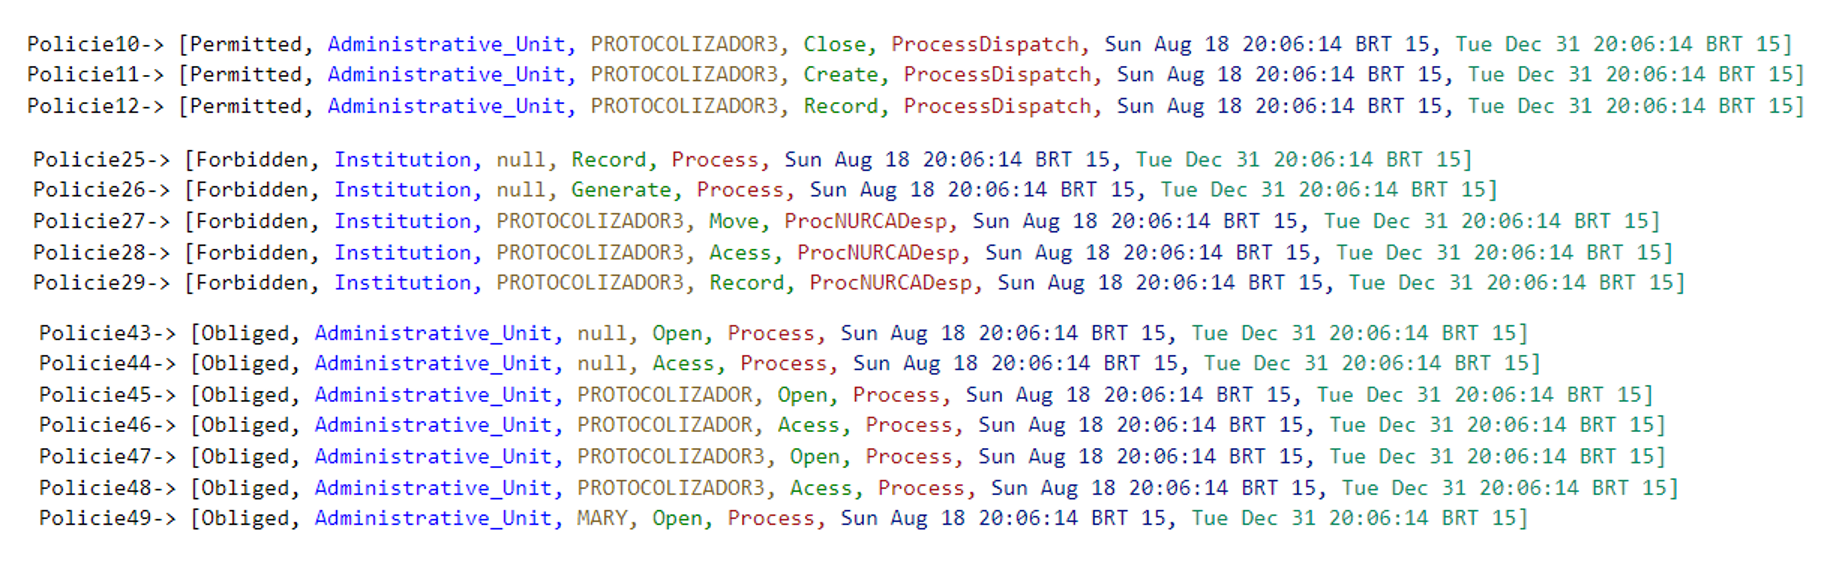
\includegraphics[width=.8\textwidth]{imagens/modelo_politica.png}}
	
	{\scriptsize Fonte: compilação do autor}
	\label{fig:modelo_politica}
\end{figure}

\subsection{Detecção de conflitos} \label{deteccao_conflitos}

Segundo \citeonline{kalam_organization_2003}, quando um modelo de controle de acesso inclui a possibilidade de especificar \textit{permissões}, \textit{proibições} e \textit{obrigações} podem ocorrer alguns conflitos entre políticas. 

Os conflitos podem acontecer quando diferentes conjuntos de condições resultam em \textit{permitir} e \textit{negar} simultaneamente, ao mesmo papel, à mesma solicitação, ou \textit{proibir} e \textit{obrigar} o mesmo papel, à mesma solicitação, isto é, quando os \textit{objetivos} de duas ou mais políticas \textit{não podem ser atendidos simultaneamente} \cite{cuppens_high_2007}.

\subsubsection{Classificação dos conflitos}

De acordo com \citeonline{cuppens_high_2007}, \citeonline{sloman_security_2002} e \citeonline{lupu_conflicts_1999}, os conflitos classificam-se, principalmente em: \begin{itemize}
	\item \textit{conflito de modalidade} que decorre de políticas de propriedades contrárias; 
	\item \textit{conflito em potencial} surge da tripla sobreposição de sujeitos, ações e objetos de políticas de predicados opostos;
	\item \textit{conflito de redundância} que surge da precedência de execução dadas a certas políticas e
	\item \textit{conflito específico de aplicação} que ocorre quando ações antagônicas são atribuídas para a mesma entidade (sujeito ou papel) mediante controles externos específicos, expressos como metapolíticas que agem como contenções para políticas permitidas.
\end{itemize}

Neste trabalho, para o modelo de política proposto, não abordam-se os conflitos de redundância já que ordens de precedência não são tratadas. Todas as outras modalidades de conflitos são examinadas e utilizadas.

Assim como em \citeonline[p. 24]{sarkis2017}, neste trabalho, os conflitos em potencial são denominados \textbf{conflitos diretos} e os conflitos de aplicação são abarcados pelos chamados \textbf{conflitos indiretos}.

\subsubsection{Conflitos Diretos e Indiretos}
\citeonline{dunlop_dynamic_2002} usam uma abordagem para os conflitos diretos e simples que será replicada neste trabalho. Diz-se que duas regras estão em conflito \textit{quando o cumprimento de uma das regras viola a outra e vice-versa}. Ou seja, a verificação se há o conflito é feita entre duas políticas que possuem modalidades contraditórias ou antagônicas, definidas na mesma organização, executadas pelos mesmos sujeitos, efetuando a mesma ação em relação a um objeto específico.

Exemplo de um \textit{\textbf{conflito direto}}:

{\scriptsize \texttt{ \{P1= {\underline{Permitido}, na Universidade X, Ana Ester, acessar processos administrativos\} }}}

{\scriptsize \texttt{ \{P2= {\underline{Proibido}, na Universidade X, Ana Ester, acessar processos administrativos\} }}}

Os exemplos acima mostram que quando uma política proíbe e a outra permite um sujeito de realizar uma ação estabelecida sobre um objeto específico em uma organização particular ocorre um \underline{conflito direto}. O conflito, segundo \citeonline{autrel_motorbac_nodate}, pode ser identificado diretamente utilizando a sobreposição dos atributos das políticas.

Já em um \underline{conflito indireto,} as políticas conflitantes regulam ações diferentes (mas relacionadas) executadas por distintos sujeitos (porém, relacionados) sobre objetos desiguais (mas, relacionados) em organizações diferentes (mas, relacionadas) \cite[p.24]{sarkis2017}.

Além disso, um conflito indireto pode ainda ocorrer, mesmo quando as políticas em conflito não têm modalidades contraditórias ou contrárias.

Ex:

{\scriptsize \texttt{P3 = {Obrigado, Empresa E, \underline{Funcionário, receber}, avaliação, mensal}}}

{\scriptsize \texttt{P4= {Permitido, Empresa E, \underline{Analista, conceder}, avaliação, mensal}}}

Este conflito não seria detectado diretamente, porém há um conflito se considerarmos os relacionamentos.

A capacidade de um sistema reconhecer um estado inconsistente em andamento ou em potencial é denominada \textbf{detecção de conflitos.}

Para \citeonline{sarkis2017},
\begin{citacao}
	detectar conflitos entre políticas de controle de acesso é o primeiro passo para buscar inibir o surgimento de erros no sistema relativo às políticas aplicadas, tendo em vista que as políticas sem conflitos refletem corretamente o plano de segurança do sistema.
\end{citacao}

Ainda segundo \citeonline[p.25]{sarkis2017}, ``Para um sistema baseado em políticas trabalhar de forma eficaz é importante ter um meio de detectar e resolver os conflitos que possam surgir''. Torna-se, assim, indispensável a utilização de abordagens que analisem previamente a existência de conflitos como o proposto nesta dissertação.

Na próxima seção os conceitos de mineração de dados utilizado neste trabalho serão descritos.


\section{Mineração de Dados}\label{mineracao_dados}
Uma das características de nossa era é produção de dados em grande volume, velocidade e variedade de todas as formas, por dispositivos espalhados em toda parte. Entretanto, dados, mesmo em grande quantidade, são apenas dados. É preciso produzir informação e conhecimento para explorar as vantagens que essa massa pode trazer. O dado necessita ser, de alguma forma, analisado, tratado para que informações e conhecimento possam ser, deles, extraídos \cite{aprenda_mineracao_fernando_amaral16} \cite{ferrari2017}.

Conforme \citeonline{fayyad1996}:
\begin{citacao}
	 Os computadores permitiram que os humanos coletassem mais dados do que podemos digerir, é natural [,portanto,] recorrer a técnicas computacionais para nos ajudar a desenterrar padrões e estruturas significativas a partir dos numerosos volumes de dados. Por isso, [a mineração de dados] é uma tentativa de resolver um problema que a era da informação digital transformou em realidade para todos nós: sobrecarga de dados.
\end{citacao}

Para \citeonline{Boscarioli2017}, a \textit{mineração de dados} pode ser definida como um processo automatizado ou semiautomatizado de explorar grandes bases de dados de forma extensiva, com o objetivo de encontrar padrões relevantes que ocorrem nos dados e que sejam significativos para embasar a absorção de informação importante, contribuindo para a geração de conhecimento. 

Para \citeonline{fayyad1996}, o termo ``mineração de dados'' tem sido usado  por estatísticos, analistas de dados e comunidades de sistemas de informações ganhando popularidade no campo do banco de dados. Já o termo \textit{descoberta de conhecimento em bancos de dados [}(KDD, da sigla em Inglês)] foi cunhada para enfatizar que o conhecimento é o produto final de uma descoberta baseada em dados. Está sendo utilizado nos campos de IA e aprendizado de máquina.


\subsection{KDD - Knowledge Discovery in Databases}
Assim, a mineração de dados é parte integrante de um processo mais amplo, conhecido como descoberta de conhecimento em bases de dados (\textit{Knowledge Discovery in Databases}, ou \textit{KDD})\cite{fayyad1996}. 

Embora se use \textit{mineração de dados} como sinônimo de KDD, a terminologia é empregada para a etapa de \textit{descoberta}  do processo de KDD, que inclui a \textit{seleção} e \textit{integração} das bases de dados, a \textit{limpeza} da base, a \textit{seleção e transformação} dos dados, a \textit{mineração}(propriamente) e a \textit{avaliação} dos dados. \cite{ferrari2017}\cite{Boscarioli2017}.

Assim, a mineração de dados  é definida em termos de esforços para a descoberta de padrões em bases de dados. A partir destes padrões descobertos, há condições de se gerar conhecimento útil para um processo de tomada de decisão (ou a geração de conhecimento para esta tomada).

Mais especificamente, KDD (\textit{Knowledge Discovery in Database}) é um processo de busca de conhecimento em bancos de dados e, de modo geral, consiste de uma sequência iterativa de passos (ou \textbf{etapas})\footnote{O processo de KDD, segundo \cite{fayyad1996} é composto por: \textit{Seleção de dados; Pré-processamento; Transformação; Mineração; Análise e assimilação de resultados}}: limpeza de dados; integração dos dados; seleção, transformação e mineração dos dados; avaliação dos padrões e apresentação e assimilação do conhecimento. Este processo é iterativo e, em alguma etapa, pode-se voltar para uma anterior \cite{Boscarioli2017}.

A \autoref{fig:processo-KDD} mostra o funcionamento iterativo do processo de KDD (\textit{Knowledge Discovery in Database}) -  Descoberta de Conhecimento em Bases de Dados.

\begin{figure}[h!]
	\centering
	\caption{Etapas do processo de descoberta do conhecimento em bases de dados - KDD}
	\fbox{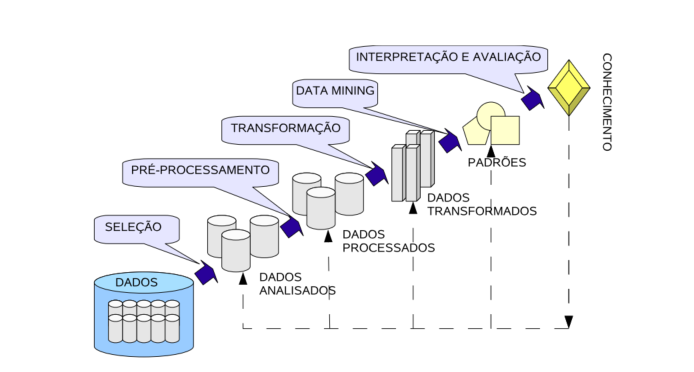
\includegraphics[width=.6\textwidth]{imagens/processo-KDD.png}}
	
	{\scriptsize Fonte: \cite[p. 7]{vasconcelos_aplicacao_2018}}
	\label{fig:processo-KDD}
\end{figure}

Neste trabalho as tarefas de seleção e transformação dos dados farão parte da etapa chamada de pré-processamento de acordo com, \citeonline{Boscarioli2017} e serão descritas com maior riqueza de detalhes no \autoref{resultados}.

\subsection{Modelo de conhecimento}\label{modelo_conhecimento}
O termo \textbf{modelo de conhecimento} (ou hipótese) é utilizado na literatura (e neste trabalho) para fazer referência a um padrão ou conjunto de padrões descobertos (que é, enfim, o \textit{propósito} do processo de KDD). Estes padrões são conhecimentos representados segundo as normas sintáticas de alguma linguagem formal. Estes padrões podem ser classificados em dois tipos: \textit{preditivos} e \textit{descritivos} \cite{ferrari2017}.

O intuito dos preditivos é resolver um problema específico de prever os resultados ou valores de um ou mais atributos, em função dos valores de outros atributos. Os descritivos (ou informativos) tem o intuito de apresentar informações interessantes e importantes sobre os dados que um especialista de domínio possa não conhecer\cite{goldschmidt2005}. 

Modelos de conhecimento compostos exclusivamente por padrões preditivos são chamados de modelos preditivos, enquanto que modelos descritivos são modelos de conhecimento compostos por padrões descritivos \cite{Boscarioli2017}.

Para \citeonline{minewiskan_modelos_nodate}, \begin{citacao}
	Um modelo de mineração é criado aplicando-se um algoritmo a dados, mas é mais que um algoritmo ou um contêiner de metadados: é um conjunto de dados, estatísticas e padrões que podem ser aplicados a novos dados para gerar previsões e fazer inferências sobre relações.
\end{citacao}

Neste contexto, este trabalho se concentra, portanto, em criar modelos de forma a detectar, mediante o uso de técnicas da mineração de dados (e aprendizagem de máquina) os conflitos entre as políticas de controle de acesso de um sistema. Diversos modelos serão desenvolvidos e confrontados usando-se vários algoritmos e técnicas analisados com métricas específicas.

\subsubsection{Arquitetura do modelo}\label{arquitetura_modelo}

Segundo \citeonline{minewiskan_modelos_nodate}, ``Um modelo de mineração obtém dados de uma estrutura de mineração e analisa esses dados usando um algoritmo de mineração de dados''. Entretanto, é importante diferenciar a estrutura e o modelo de mineração. Ainda de acordo com \citeonline{minewiskan_modelos_nodate}, a \textit{estrutura} armazena informações que definem a fonte de dados, já um \textit{modelo} de mineração armazena informações derivadas do processamento estatístico dos dados, como padrões encontrados em decorrência da investigação.

Assim, o modelo fica ``limpo'' até que os dados que foram guarnecidos pela estrutura de mineração sejam processados e avaliados. Depois de produzido o modelo contém \textit{metadados}, resultados e associações e pode, então, ser utilizado para a obtenção de conhecimento.

A arquitetura pode conter também, variáveis, \textit{hiperparâmetros}, definições do modelo, filtros utilizados e, claro, o algoritmo utilizado na tarefa de análise dos dados. \cite{deep_learning_book_2019}.

\section{Aprendizagem de máquina} \label{aprendizagem_maquina}
Segundo \citeonline[p. 10]{goldschmidt2005}, \begin{citacao}
	um dos passos do processo de KDD, o de extração de padrões (ou Mineração de Dados) utiliza métodos de Aprendizado de Máquina (AM) [ou \textit{Machine Learning} - ML] para encontrar regularidades, padrões ou conceitos em conjuntos de dados.
\end{citacao}

A principal diferença, segundo os autores, \citeonline{goldschmidt2005} entre Aprendizagem de Máquina e KDD reside no fato de ``grande parte da literatura em AM se concentra apenas no mecanismo de descoberta de padrões e/ou conceitos, sem se preocupar com o grau de utilidade''. Já em KDD, ainda segundo \cite{goldschmidt2005}, ``os padrões extraídos são avaliados para aferir sua utilidade para o usuário em relação à tomada de decisão''. Ou seja, o aprendizado na Aprendizagem de Máquina é um atividade-fim enquanto o aprendizado no KDD é uma atividade-meio para a obtenção do conhecimento.

\subsection{Definição}
Aprendizado de máquina ou \textit{machine learning} é um braço da Inteligência Artificial que emprega técnicas e algoritmos na criação de modelos computacionais dos quais a característica principal é a capacidade de descobrir padrões em um grande volume de dados ou de melhorar o desempenho de uma determinada tarefa através da experiência (do \textit{reforço}).\cite{mohri_foundations_2018} \cite{alpaydin_introduction_2014} \cite{swamynathan_mastering_2019}

Então, de acordo com \citeonline[p. 278]{baeza-yates_recuperacao_2013}, ``os padrões aprendidos, que podem ser bem complexos, são então usados para fazer predições relativas a dados ainda não vistos e novos''.

Nas palavras de Arthur Lee Samuel \citeonline{wiederhold_arthur_1992}, considerado um dos pioneiros na área de inteligência artificial, aprendizado de máquina é ``o campo de estudo que dá aos computadores a capacidade de aprender sem serem explicitamente programado''. \cite[p. 89]{simon_too_2013}. 

Aprendizado de máquina tem sido aplicado na automatização de funções que para os humanos são executadas intuitivamente, mas que são difíceis de definir formalmente. \cite{sarkar_2017}

Assim, de forma geral, a aprendizagem de máquina tem por objetivo estudar e desenvolver métodos computacionais para obter sistemas capazes de adquirir conhecimento de forma automatizada. \cite{lima_ia_2016}.

A capacidade de determinados algoritmos tem de aprender a partir de exemplos é chamado de \textbf{aprendizado indutivo}. Estes algoritmos aprendem relacionamentos eventualmente existentes entre os dados, mostrando o resultado nos modelos de conhecimento gerado. \cite{goldschmidt2005}\cite{alpaydin_introduction_2014}

Conforme \citeonline[p. 279]{baeza-yates_recuperacao_2013}, os algoritmos de aprendizado de máquina ``são fundamentalmente dependentes de uma fase de aprendizado, a qual é usada para produzir um modelo ou uma função que codifica padrões presentes nos dados de entrada''.

Então, dependendo de qual é a abordagem de aprendizado usada, os algoritmos de aprendizado de máquina podem ser, basicamente de 3 principais tipos, que são: a aprendizagem supervisionada, a aprendizagem não-supervisionada e a aprendizagem por reforço \footnote{Há ainda os tipos de aprendizado \textit{semissupervisionado} e a \textit{transdução} (ou inferência transdutiva) que não serão discutidos neste trabalho}. \cite{Norvig2013} \cite{baeza-yates_recuperacao_2013}. 

Na \textbf{aprendizagem não-supervisionada} o modelo/hipótese busca padrões na entrada, embora não seja fornecido nenhum \textit{feedback} explícito. Portanto, na abordagem não-supervisionada não há, nos dados, uma classe, não há um rótulo prévio, ou seja, não existe a informação da saída desejada. O processo de aprendizado busca identificar regularidades entre os dados e não é necessária a divisão prévia dos dados em dados de treinamento, validação e teste.  A tarefa mais comum de aprendizagem não supervisionada é o agrupamento. mas, os algoritmos de aprendizagem não-supervisionada incluem ainda, modelos de redes neurais, análise de componentes independentes e o já citado \textit{clustering} (agrupamento) \cite{Norvig2013} \cite{Boscarioli2017} \cite{goldschmidt2005} \cite{aprenda_mineracao_fernando_amaral16}

Na \textbf{aprendizagem supervisionada} o modelo/hipótese observa alguns exemplos de pares de entrada e saída, e aprende uma função (ou modelo) que faz o mapeamento entre a entrada e a saída. Portanto, ela compreende a abstração de um modelo a partir dos dados apresentados na forma de pares ordenados (\textit{entrada, saída, saída desejada}). Há, assim, uma \textit{classe}, ou um atributo especial com o qual se pode comparar e validar o resultado. Esta categoria de aprendizagem de máquina requer uma função de aprendizado dos dados de treinamento fornecidos como entrada. Esses dados, então, são usados para para aprender uma função de classificação que pode, assim, ser usada para realizar predições de classes para dados ainda não vistos ou novos. \cite{Norvig2013} \cite{luger_inteligencia_2015} \cite{baeza-yates_recuperacao_2013}

Na \textbf{aprendizagem por reforço}, aprende-se a partir de uma série de reforços --- recompensas ou punições. Não está disponível, geralmente, na aprendizagem por reforço, para o algoritmo de aprendizado de máquina, um conjunto de dados para treinamento. O aprendizado se dá, então, pela interação com o ambiente que se deseja atuar por um determinado período com o objetivo de melhorar o desempenho de uma determinada tarefa. \cite{Norvig2013} \cite{aprenda_mineracao_fernando_amaral16} \cite{silva_restaurante_2019}	

\section{Algoritmos de classificação}
A classificação é considerada uma das tarefas principais do processo de aprendizagem de máquina, sendo, inclusive, a tarefa mais comum. \cite{amaral_introducao_2018} \cite{fayyad1996}.

Segundo, \citeonline[p. 86]{amaral_introducao_2018}, ``Na classificação, os dados devem possuir uma \textit{classe} a qual queremos prever''. Conforme \citeonline{Rocha2012}, ``o termo \textit{classe} deve ser usado quando existe informação sobre quantas e quais são as partições presentes em um conjunto de dados, bem como qual exemplar pertence a qual partição''

Comumente denomina-se \textit{classificação} o processo pelo qual se determina uma função de mapeamento capaz de indicar a qual classe pertence algum exemplar de um domínio sob análise, baseando-se em um conjunto já classificado. \cite{Boscarioli2017}.

Assim, de acordo com \citeonline{classification2013}, classificação é uma técnica de mineração de dados (aprendizado de máquina) usada para prever a associação ao grupo para instâncias de dados. É, segundo \citeonline{aprenda_mineracao_fernando_amaral16} e \citeonline{performance_classification2013}, como citado anteriormente, a tarefa mais utilizada em mineração de dados. Além de ser a mais complexa e a que possui a maior quantidade de algoritmos disponíveis, conforme descrito em \citeonline{classification2013}.

A classificação é uma das tarefas \textit{preditivas} de Mineração de Dados e aprendizado de máquina. Tarefas de predição consistem na análise de um \textit{dataset} (conjunto de dados), descritos por atributos e rótulos associados com o objetivo de descobrir um \textbf{modelo} capaz de mapear corretamente cada um dos dados a seus rótulos apropriadamente. Esse objetivo é alcançado por meio de técnicas, normmalmente, chamadas de supervisionadas. Este tipo de análise preditiva pode ser dividida em \textit{categórica}, também chamada de \textit{classificação} ou em \textit{numérica}, também chamada de regressão. Cf. \citeonline{Boscarioli2017}  e \citeonline{classification2013}, também exposto em \citeonline{ferrari2017} e \citeonline{goldschmidt2005}

\underline{Formalmente}, a tarefa de classificação pode ser descrita como a busca por uma função de mapeamento para um conjunto $X$ de vetores de entrada (ou, exemplares --- os dados) $\vec{x_i} \in E^d$ para um conjunto finito de rótulos $C$ de cardinalidade $c$. A função $F$ é, então, definida como $F: E^d \times W \rightarrow C$, em que $d$ é a dimensão do espaço $E$, ou seja, a quantidade de coordenadas do vetor $\vec{x_i}$, e $W$ é um espaço de parâmetros ajustáveis por meio do algoritmo de indução supervisionada. \cite{Boscarioli2017}

Pode ser dividida em, ao menos, duas categorias: \textit{classificação binária} e \textit{classificação multiclasse}. Na binária, a cardinalidade $c$ é 2. Para o caso em que $c > 2$, o problema é considerado de múltiplas classes. \cite{Boscarioli2017} \cite{classification2013}

Os textos de \citeonline{classification2013}, \citeonline{performance_classification2013}, além dos de \citeonline{Wolpert:1996}, \citeonline{classification_survey2012} e \citeonline{using_data_mining2012}  trazem reflexões, técnicas, comparações e explicações detalhadas de muitos algoritmos de classificação, entre eles, árvores de decisão, k-vizinhos mais próximos, Naive Bayes e Redes Bayesianas, Redes Neurais Artificiais, Máquinas de Vetores de Suporte (SVM) entre outros.   

Sobre \textit{teoria da aprendizagem} e \textit{algoritmos de classificação} há uma discussão em \citeonline{Norvig2013} sobre qual seria, em relação às hipóteses de modelos de aprendizagem, aquela (ou aquelas) que melhor se ajuste aos dados futuros. Os autores citam a \textbf{\textit{suposição de estacionaridade}}, ou seja, que há uma distribuição de probabilidade sobre os dados que permanece estacionária ao longo do tempo. Supõe-se, portanto que cada exemplo de ponto de dados (antes de conhecê-lo) é uma variável aleatória $E_j$ cujo valor observado $e_j = (x_j, y_j)$ é amostrado da distribuição e é independente dos exemplos anteriores. 

Assim:
\begin{equation}
	P (E_j|E_{j-1},E_{j-2}, ... ) = P(E_j) \textrm{,} 
\end{equation}

e cada exemplo tem uma distribuição de probabilidade anterior idêntica:

\begin{equation}
P(E_j) = P(E_{j-1}) = P(E_{j-2}) = \dots 
\end{equation}

Estes exemplos são chamados de \textit{independentes e identicamente distribuídos} ou \textbf{i.i.d}. Esta suposição é, segundo os autores, \underline{necessária} para \textit{tentar a previsão sobre o futuro dos dados}. Há claro, ainda em \citeonline{Norvig2013}, um alerta sobre o fato de ser possível a aprendizagem ocorrer caso haja pequenas alterações (lentas) na distribuição.

Outro fato importante para a definição e avaliação da escolha da melhor hipótese (modelo) de um algoritmo de classificação é definir o ``melhor ajuste''. Em seu conhecido livro de Inteligência Artificial, os autores \citeonline{Norvig2013} definem a \textbf{taxa de erro} de uma hipótese como uma métrica importante para definir o ``melhor ajuste'' de um modelo/hipótese.

\subsubsection{Taxa de erro}\label{taxa_erro}

A taxa de erro é, assim, a proporção de erros que o algoritmo classificador comete --- a proporção de vezes que $h(x)\neq y$ para o exemplo $(x,y)$ --- sendo $h(x)$ a função que mapeia uma \textit{hipótese/model}o $h$ com a \textit{previsão/valor} conhecido $y$. Nem sempre, como alerta, \citeonline{Norvig2013}, uma hipótese/modelo $h$ que tenha uma taxa de erro baixa no conjunto de treinamento generaliza bem e se comporta eficientemente para dados não conhecidos. A forma de testar o algoritmo é importante. Para isso há, na literatura, algumas técnicas que são utilizadas como estratégia de treinamento, validação e teste.

\subsubsection{Estratégias de validação}\label{estrategias_validacao}

Como citado por \citeonline{Norvig2013} e \citeonline{luger_inteligencia_2015} entre diversos autores e, cf. \citeonline[p. 125]{Boscarioli2017}, 
\begin{quote}
	independentemente da medida de avaliação a ser usada para atestar a qualidade de um modelo, não é adequado avaliá-lo [apenas] por seu desempenho em relação aos exemplares apresentados no processo de treinamento (indução). É sempre necessário saber como o modelo se comporta quando aplicado a exemplares que ainda não conhece, ou seja, não usados no processo de sintonização de seus parâmetros.
\end{quote}

Essa observação, claro, é porque modelos preditivos, dependendo de como são criados, podem levar ao \textit{\textbf{overfitting}} (sobreajuste). O fenômeno do sobreajuste ocorre, cf. \citeonline{Boscarioli2017} ``quando o modelo preditivo é gerado de forma a representar os exemplares usados para sua geração com uma fidelidade mais alta que o necessário''. 

Assim, modelos sobreajustados (ou superajustados) não são capazes de realizar predições adequadas para dados novos. Busca-se, na construção de modelos preditivos, uma maior \textit{generalização} e no caso do sobreajuste o fenômeno contrário ocorre. 

A maior causa de sobreajuste é quando os dados de treinamento não representam fielmente os dados novos (ou de produção) ou por serem diferentes (caso de dados antigos, por exemplo) ou por não serem significativos (poucos dados)\footnote{ é possível também o sobreajuste devido a \textit{ruídos} nos dados, pelo uso de um modelo de forma inapropriada ou de uma \textit{classe rara} \cite[p.35]{aprenda_mineracao_fernando_amaral16}}. A \autoref{fig:overfitting} mostra um modelo preditivo em que o lado direito representa um modelo sobreajustado e o lado esquerdo um modelo regularizado para o mesmo \textit{dataset}.

\begin{figure}[h!]
	\centering
	\caption{Modelo sobreajustado e regularizado para o mesmo \textit{dataset}.}
	\fbox{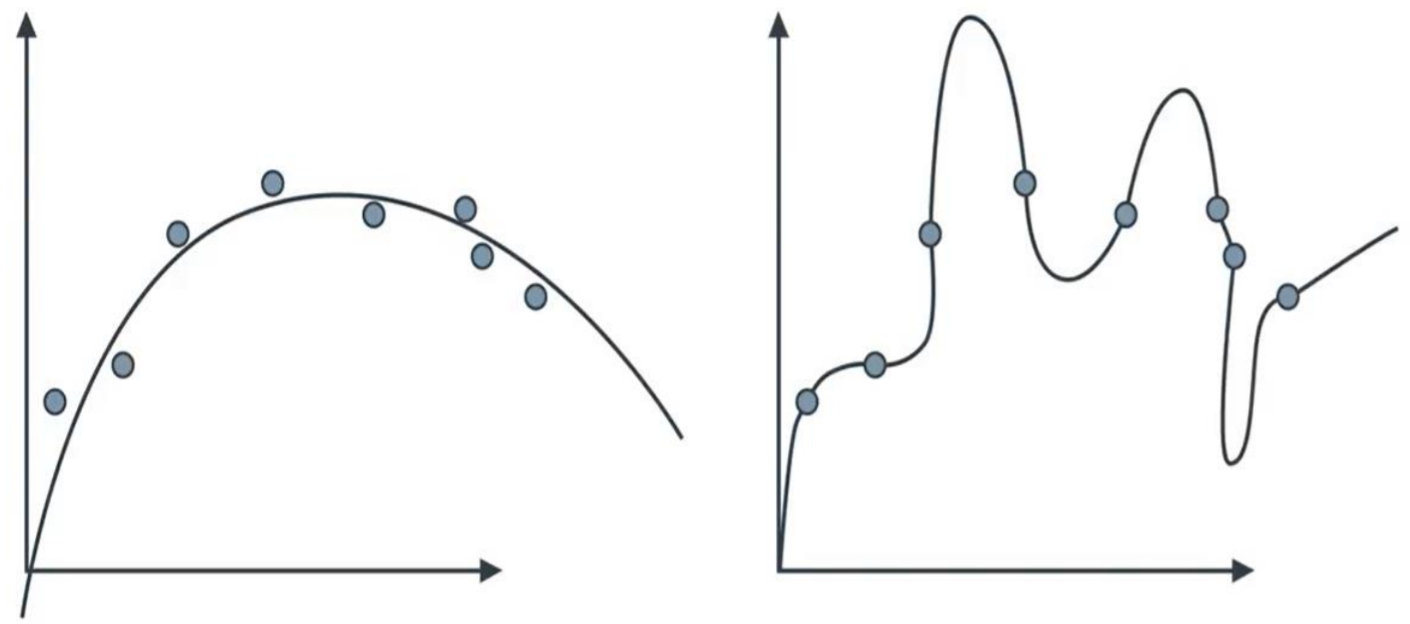
\includegraphics[width=.6\textwidth]{imagens/overfitting.png}}
	
	{\scriptsize Fonte: baseado no encontrado em \cite{over_and_underfitting_2019}}
	\label{fig:overfitting}
\end{figure}

Nas palavras de \citeonline[p. 95]{amaral_introducao_2018}, ``o processo de construção de um modelo de aprendizado de máquina busca, obviamente, maximizar a precisão e minimizar a taxa de erros''. Para tanto, a literatura cita diversas técnicas e estratégias para a avaliação de modelos preditivos. Autores diversos, como \citeonline{Boscarioli2017}, \citeonline{aprenda_mineracao_fernando_amaral16}, além de  \citeonline{data_science_do_zero2016} e \citeonline{ferrari2017} citam, geralmente, como estratégia de treinamento, validação e teste as seguintes técnicas:

\begin{itemize}
	\item Resubstituição;
	\item Holdout;
	\item Validação cruzada;
	\item Bootstrap;
\end{itemize}

Na \textbf{\underline{resubstituição}}, segundo \citeonline{Boscarioli2017}, as medidas de avaliação dos classificadores são aplicadas no próprio conjunto de dados usados para indução do modelo. Essa técnica, embora tenha alguns vantagens discutidas em \citeonline{ferrari2017} e \citeonline{Boscarioli2017}, pode levar ao, já citado, sobreajuste (\textit{overfitting}) e é discutido em \citeonline{data_science_do_zero2016}, também em \citeonline{aprenda_mineracao_fernando_amaral16} e \citeonline{Norvig2013}. Como já afirmado anteriormente, o sobreajuste é quando se produz um modelo de bom desempenho com os dados de treinamento, mas que não lida bem com novos dados.

Na técnica de \textbf{\underline{Holdout}}, pressupõem-se uma divisão, ou criação de dois subconjuntos de dados distintos, a partir do conjunto de dados disponível pra uso na indução do modelo/hipótese. Um desses subconjuntos será usado para treinamento (indução) do modelo de previsão e o segundo, para teste após o término do treinamento e, consequentemente, na aplicação das medidas de avaliação do modelo/hipótese. \cite{Boscarioli2017}

A \autoref{fig:img_holdout} mostra o funcionamento da técnica de holdout de forma mais detalhada
\begin{figure}[h!]
	\centering
	\caption{Funcionamento da técnica holdout.}
	\fbox{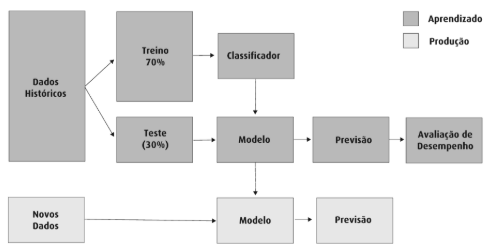
\includegraphics[width=.6\textwidth]{imagens/hold_out.png}}
	
	{\scriptsize Fonte:\cite{aprenda_mineracao_fernando_amaral16}}
	\label{fig:img_holdout}
\end{figure}

Na estratégia de \textbf{\underline{validação cruzada}}, todos os dados farão parte, em algum momento, do conjunto de dados usado no teste do modelo/hipótese. A ideia é que cada exemplo sirva duplamente --- como dados de treinamento e dados de teste. Primeiro divide-se o conjunto em $k$ subconjuntos iguais. Em seguida realiza-se $k$ rodadas de aprendizagem; em cada iteração $\frac{1}{k}$ dos dados é retido como conjunto de teste e os exemplos restantes são usados como treinamento. 

Valores populares de $k$ são 5 e 10 --- o suficiente para uma estimativa estatisticamente provável que seja precisa a um custo 5-10 vezes maior no tempo de computação. Há também o extremo do $k = n$, também conhecido como \textbf{validação cruzada com omissão de um}. O método de validação cruzada permite que o modelo/hipótese seja avaliado uma série de vezes, cada série sendo conhecida como partição (ou \textit{fold}). Ao final, a avaliação pode ser realizada aplicando medidas estatísticas como média, desvio-padrão e intervalo de confiança ao conjunto de $k$ avaliações obtidas ou somando-se os desempenhos obtidos pelos $k$ modelos gerados e dividindo essa soma pelo número de exemplares original. \cite{Norvig2013}\cite{Boscarioli2017}\cite{ferrari2017} \cite{aprenda_mineracao_fernando_amaral16}

A \autoref{fig:img_cross_validation} mostra um exemplo didático de como funciona a validação cruzada. Os dados que não fazem parte do conjunto de teste em cada rodada são utilizados no treinamento.

\begin{figure}[h!]
	\centering
	\caption{Funcionamento da técnica \textit{cross validation}}
	\fbox{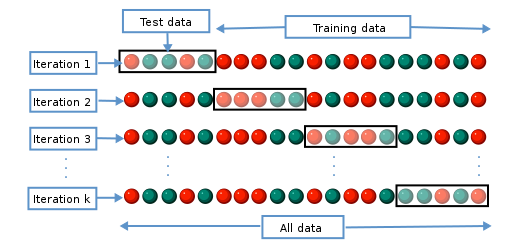
\includegraphics[width=.6\textwidth]{imagens/cross_validation.png}}
	
	{\scriptsize Fonte:\cite{fold_cross_validation:k-fold_nodate}}
	\label{fig:img_cross_validation}
\end{figure}

Já a técnica de \textit{\textbf{\underline{Bootstrap}}} funciona de forma  parecida à estratégia \textit{holdout}. Ela também usa dois conjuntos, um de treinamento e outro para teste, porém durante o processo de formação dos subconjuntos, exemplares que já foram sorteados podem novamente serem contemplados, com probabilidade igual. É uma estratégia que permite, portanto, a reposição.

Neste trabalho, todos os algoritmos de classificação usados foram testados usando as técnicas de resubstituição, \textit{holdout} (com taxas de 70-30, 75-25 e 60-40), além de \textit{cross-validation} com 3, 5 e 10 folds. 

Como explicado em \citeonline{WolpertMacready} e \citeonline{Wolpert:1996} não existe um algoritmo de aprendizado superior a todos os demais quando considerados todos os problemas de classificação possíveis (teorema \textbf{NFL}, ou \textit{No Free Lunch}), portanto, variações foram executadas nos experimentos em todas técnicas avaliadas, alterando-se os padrões para chegar a métricas e medidas de avaliação mais eficientes.

\subsubsection{Medidas de avaliação}\label{medidas_avaliacao}

Para \citeonline{castro_supervised_2011}, 
\begin{quote}
	Tradicionalmente, a métrica usada na avaliação e seleção de modelos de classificação é a acurácia (ou taxa de erro) estimada em relação a um dado conjunto de teste. Essa metodologia é justificada pela formulação padrão do problema do aprendizado supervisionado que visa a minimização da probabilidade do erro global. 
\end{quote}

Há, porém, conforme \citeonline{Boscarioli2017}, \citeonline{aprenda_mineracao_fernando_amaral16}, \citeonline{classification2013} e \cite{classification_survey2012} diversas medidas usadas na avaliação de classificadores. 

A que será usada neste trabalho (com o objetivo de minimizar a probabilidade do erro global) é a, já citada, acurácia ou taxa de classificações corretas. 

A métrica acurácia é dada, portanto, por:

\begin{equation}\label{acuracia}
	\textrm{Acurácia} = |y-f(\aleph)=0|\textrm{,}
\end{equation}

em que $|\cdot|$ representa a contagem de vezes em que $\cdot$ é verdadeiro, $f$ é o modelo preditivo, $\aleph$ é o subconjunto de dados sob o qual o modelo está sendo avaliado, $f(\cdot)$ é a classificação fornecida pelo modelo preditivo para cada um dos exemplares (dos dados), e $y$ é a classe esperada como resposta. \cite[p. 129]{Boscarioli2017}

A acurácia de um classificador também pode ser descrita em termos do \textbf{erro de generalização} $\xi_g$, e uma função de perda binária e, portanto, ser interpretada como a probabilidade de ocorrer uma classificação correta. Dessa forma:

\begin{equation}
\textrm{Acurácia}_g=1 - \xi_g
\end{equation}

Ou seja, a acurácia é, basicamente o número de acertos (positivos) divido pelo número total de exemplos. Será a métrica mais usada para avaliar os classificadores neste trabalho.

Há, entretanto, em modelos preditivos que trabalham com dados numéricos (como as redes neurais e o SVM), pode-se utilizar uma função de perda contínua, capaz de medir o erro entre a resposta obtida pelo modelo preditivo e a resposta aguardada. \cite{Boscarioli2017} \cite{deep_learning_book_2019}.

Para \citeonline{nn_smithing_1999}
\begin{citacao}
	A função de custo reduz todos os aspectos bons e ruins de um sistema complexo a um único número, um valor escalar, o que permite ranquear e comparar as soluções candidatas.
\end{citacao}

Algumas funções de perda (\textit{loss functions}), comuns, neste contexto são: \cite{Boscarioli2017}

\begin{equation}\label{erro_absoluto}
	\textrm{\textit{Erro absoluto}}=\sum_{<\vec{x}_i, y_i> \in \aleph} |y_i - f(\vec{x}_i)|
\end{equation}

\begin{equation}\label{erro_quadratico}
\textrm{\textit{Erro quadrático}}=\sum_{<\vec{x}_i, y_i> \in \aleph} (y_i - f(\vec{x}_i))^2
\end{equation}

\begin{equation}\label{erro_absoluto_medio}
\textrm{\textit{Erro absoluto médio}}=\sum_{<\vec{x}_i, y_i> \in \aleph} |y_i - f(\vec{x}_i)|/m
\end{equation}

\begin{equation}\label{erro_quadratico_medio}
\textrm{\textit{Erro médio quadrático}}=\sum_{<\vec{x}_i, y_i> \in \aleph} (y_i - f(\vec{x}_i))^2/m
\end{equation}

Onde $m$ é a quantidade de instâncias existentes em $\aleph$. 

\citeonline{Boscarioli2017}, \citeonline{amaral_introducao_2018} além de \citeonline{deng_improved_2016} e \citeonline{ruuska_evaluation_2018} afirmam que é importante analisar o tipo de erro que o modelo está cometendo e, principalmente, no caso de classificadores binários, é possível observar que, mesmo com uma acurácia alta o classificador pode não estar respondendo de forma adequada. 

Para realizar esse tipo de análise, os autores citados no princípio deste parágrafo, citam que uma ferramenta adequada é a \textit{\textbf{matriz de confusão}}. 

Geralmente, uma matriz de confusão tem dimensões $C \times C$, em que $C$ é o número de classes presentes no problema de classificação que está sendo avaliado. As linhas dessa matriz são indexadas seguindo as ``classes esperadas'' $(y)$, e as colunas seguindo as ``classes preditas'' $(f(x) ou \hat{y})$. 

Cada célula é um contador que é incrementado a depender do resultado da comparação de $f(x)$ e $y$. As respostas corretas do modelo geram os valores que entram na diagonal principal da matriz. \cite[p. 130]{Boscarioli2017}

A \autoref{fig:matriz_confusao} demonstra o procedimento de preenchimento de uma matriz de confusão conforme a resolução de um problema hipotético de classificação.

\begin{figure}[h!]
	\centering
	\caption{Preenchimento de uma matriz de confusão}
	\fbox{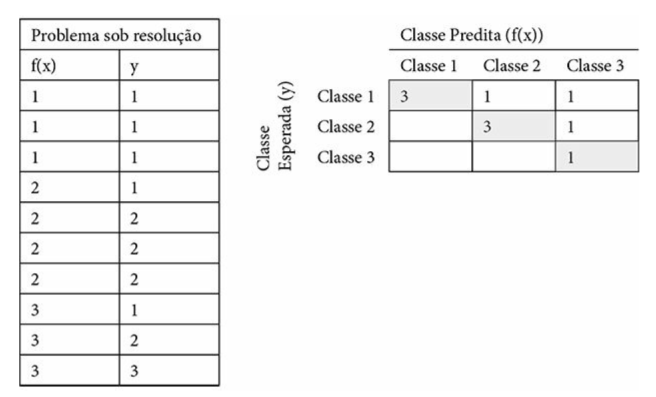
\includegraphics[width=.8\textwidth]{imagens/confusion_matrix.png}}
	
	{\scriptsize Fonte: \cite[p. 130]{Boscarioli2017}}
	\label{fig:matriz_confusao}
\end{figure}

Matrizes de confusão são, cf. \citeonline{ruuska_evaluation_2018} e \citeonline{Boscarioli2017}, particularmente úteis para avaliação de classificadores binários. Neste caso, os valores são atribuídos conforme ilustrado na figura (neste caso, as duas classes estão definidas como ``classe positiva'' e ``classe negativa''). 

\begin{figure}[h!]
	\centering
	\caption{Matriz de confusão para o caso de um classificador binário}
	\fbox{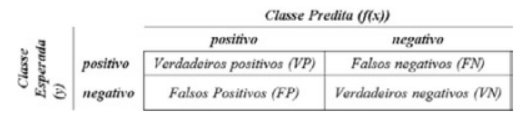
\includegraphics[width=.6\textwidth]{imagens/matriz_confusao_binario.png}}
	
	{\scriptsize Fonte: \cite[p. 131]{Boscarioli2017}}
	\label{fig:binario_matriz_confusao}
\end{figure}

Cada célula, neste caso, possui o seguinte significado:

\begin{itemize}
	\item Verdadeiro Positivo (VP): classificação correta na classe positiva. A instância pertence a classe positiva e o modelo classificou na classe positiva.
	\item Falso Positivo (FP): classificação incorreta na classe negativa. A instância pertence à classe negativa, mas o classificador a classificou como pertencente à classe positiva.
	\item Verdadeiro Negativos (VN): classificação correta na classe negativa. A instância pertence a classe negativa e o modelo classificou na classe negativa.
	\item Falso Negativo (FN): classificação incorreta na classe negativa. classificação incorreta na classe negativa. A instância pertence à classe positiva, mas o classificador a classificou como pertencente à classe negativa. 
\end{itemize}


\section{Redes Neurais Artificiais - RNA}
As redes neurais instituem um campo da ciência da computação, parte da área da inteligência artificial, que busca efetivar modelos matemáticos que se assemelhem às redes neurais biológicas. Elas apresentam capacidade de adaptar seus parâmetros como resultado da interação com o meio externo. \cite{ferneda_redes_2006}\cite{Norvig2013}

\subsection{Definição}

Para \citeonline[p. 41]{santos_um_2013} 
\begin{citacao}
	Uma rede neural artificial consiste de um sistema composto por neurônios dispostos em camadas, interligados através de pesos sinápticos construindo um sistema que simula o cérebro humano, inclusive seu comportamento. E uma técnica computacional que apresenta um modelo inspirado na estrutura neural de organismos inteligentes e que adquire conhecimento através da experiência.
\end{citacao}

De acordo com \citeonline[p. 47]{lima_ia_2016}, ``redes neurais podem ser caracterizadas como modelos computacionais com capacidades de adaptar, aprender, generalizar, agrupar ou organizar dados''.

Inicialmente, portanto, se desenvolveram como uma estratégia de simular os processos mentais humanos, como reconhecimento de imagens e sons, e após, como instrumento tecnológico e eficiente para muitas tarefas. \cite{jin_development_2002}	

Para \citeonline{obaidat_multilayer_1994}, as redes neurais artificiais podem ser usadas efetivamente para prover soluções para um amplo espectro de aplicações, incluindo mapeamento de padrões e classificação, análise e codificação de imagens, processamento de sinais, otimização, manipulação de grafos, reconhecimento de caracteres, reconhecimento automático de alvo,  	fusão de dados, processamento de conhecimento, controle de qualidade, mercado de ações, processamento de hipotecas, triagem de créditos para empréstimos entre muitos outros problemas. 

\subsection{Modelo de neurônio artificial}\label{perceptron}
Desde a década de 1940 com o trabalho de \citeonline{mcculloch_logical_1943} que se busca um modelo computacional que simule o cérebro humano e suas conexões. O interesse pela pesquisa nesta área cresceu e se desenvolveu durante os anos 50 e 60. É dessa época que \citeonline{rosenblatt_perceptron:_1958} sugeriu um método de aprendizagem para as redes neurais artificiais chamado \textit{perceptron}. 

Até o final da década de 1960 muitos trabalhos foram feitos usando o percepton como modelo, mas ao final desta década, \citeonline{minsky_perceptrons:_1969} apresentaram significativas limitações do perceptron. 

A pesquisa diminui consideravelmente nos anos seguintes (o chamado inverno da IA), porém durante  os  anos  80,  a excitação	ressurge mediante os avanços metodológicos importantes e, também, ao aumento dos recursos computacionais disponíveis. O  modelo  de  neurônio  artificial  da \autoref{fig:neuronio} é uma
simplificação do apresentado por \citeonline[p. 36]{haykin_redes_2001}

\begin{figure}[h!]
	\centering
	\caption{Modelo matemático de um neurônio}
	\fbox{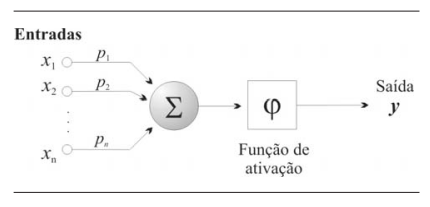
\includegraphics[width=.7\textwidth]{imagens/modelo_matematico_neuronio.png}}
	
	{\scriptsize 	Fonte: \cite[p. 36]{haykin_redes_2001}}	
	\label{fig:neuronio}
\end{figure}

O modelo da \autoref{fig:neuronio} é composto por três elementos:

\begin{itemize}
	\item  um conjunto de $ n $ conexões de entrada ($ x_1, x_2, \dots , x_n $), caracterizadas por pesos ($ p_1, p_2, \dots, p_n $);
	\item um somador ($ \sum $) para acumular os sinais de entrada;
	\item uma função de ativação ($\varphi$) que, no caso específico do neurônio apresentado por McCullock-Pitts em \citeonline{mcculloch_logical_1943} é uma função de limiar. \cite{ferneda_redes_2006} \cite{lima_ia_2016}
\end{itemize}

O comportamento das conexões entre os neurônios é simulado através de seus pesos  ($ p_1, p_2, ..., p_n $). Os valores podem ser positivos ou negativos (dependendo se a conexão é inibitiva ou excitativa. 

O efeito de um sinal proveniente de um neurônio é determinado pela multiplicação do valor do sinal recebido pelo peso da conexão correspondente ($x_i \times p_i$).

Então é efetuada a soma dos valores $x_i \times p_i$ de todas as conexões e o valor resultante é enviado para a função de ativação que define a saída ($y$) do neurônio. cf. \citeonline{Norvig2013} e \citeonline{mcculloch_logical_1943}, além de \citeonline{minsky_perceptrons:_1969}, \citeonline{ferneda_redes_2006} e \citeonline{haykin_redes_2001}

Matematicamente, a saída $y_k$ do neurônio mostrado na \autoref{fig:neuronio} é dada pela expressão abaixo:
\begin{equation}
	Y_k = \varphi(u_k) \qquad \textrm{onde} \qquad u_k = \sum_{i=1}^{n} P_{ki}X_i 
\end{equation}

A função de ativação proposta inicialmente por McCullock e Pitts em seu trabalho seminal, \citeonline{mcculloch_logical_1943} é uma função de limiar:

\begin{equation}\label{funcao_limiar}
y_k = \varphi (u_k) = \left \{ \begin{matrix}
									1, & \mbox{se }u_k > 0 \\ 
									0, & \mbox{se }u_k < 0 
								\end{matrix} 
							\right.
\end{equation}

Uma alteração importante neste modelo foi a introdução de um parâmetro polarizador (\textit{bias} ou \textit{offset}) $b_k$, conforme a \autoref{fig:bias_neuronio} cujo objetivo é deslocar o valor da informação referente à entrada líquida $u_k$, de forma a verter a função de ativação no eixo correspondente ao valor de $u_k$. Assim a saída $y_k = \varphi(u_k)$.

\begin{figure}[h!]
	\centering
	\caption{Adição de um \textit{offset} (\textit{bias}) no modelo do neurônio}
	\fbox{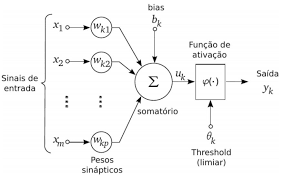
\includegraphics[width=.5\textwidth]{imagens/bias_neuronio.png}}	
	
	{\scriptsize 	Fonte: \cite[p. 58]{lima_ia_2016}}
	\label{fig:bias_neuronio}
\end{figure}

Dessa forma, o polarizador(bias) pode ser tratado como mais um peso da rede. Basta considerar um nova entrada do tipo $x_0 = 1$, com um peso associado $w_0 = b_k$, assim a representação fica sendo, considerando os pesos como $w$, de acordo com a \autoref{fig:bias_neuronio}:

\begin{equation}
	u_k = w_0 + w_1x_1 + w_2x_2; \qquad y_k = \varphi(u_k)
\end{equation}

Assim, esse neurônio pode ser empregado, segundo, \citeonline[p. 58]{lima_ia_2016}, para ``separar classes distintas de padrões de entradas para aplicações de classificações de padrões''. E prossegue: ``se a entrada líquida for maior que o limiar, o padrão dessa entrada pertence à classe 1, caso contrário, pertence à classe 0''. Analisando matematicamente o modelo \textit{perceptron}, se percebe que ele pode ser considerado um típico caso de discriminador linear. 

A fronteira de decisão para um \textit{perceptron} como o da figura \ref{fig:bias_neuronio}, dada duas entradas e a função de ativação mostrada na equação \ref{funcao_limiar} será, então, uma reta cuja equação é definida por: 

\begin{equation}\label{eq_reta}
	w_1x_1 + w_2x_2 - b = 0
\end{equation}

Portanto, cf. \citeonline{silva_redes_2016}, ``pode-se concluir que o Perceptron se comporta como um classificador de padrões cuja função é dividir classes que sejam linearmente separáveis''.

A \autoref{fig:linearmente_separavel} mostra uma reta posicionada na fronteira de separação entre as classes. Para este tipo de problema o perceptron é um classificador adequado.

\begin{figure}[h!]
	\centering
	\caption{Fronteira de separação (perceptron com duas entradas)}
	\fbox{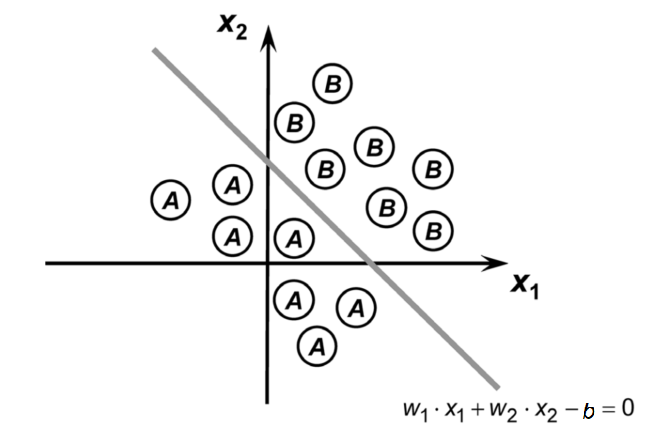
\includegraphics[width=.7\textwidth]{imagens/linearmente_separavel.png}}	

	{\scriptsize 	Fonte: \cite[p. 62]{silva_redes_2016}}
	\label{fig:linearmente_separavel}
\end{figure}

As redes neurais artificiais (\textbf{RNA}) se formam quando diversos neurônios se combinam. De forma resumida, ``uma rede neural artificial (RNA) pode ser vista como um grafo onde os nós são os neurônios e as ligações fazem a função das sinapses''. Isto está demonstrado na \autoref{fig:rna}.

\begin{figure}[h!]
	\centering
	\caption{Representação simplificada de uma RNA}	
	\fbox{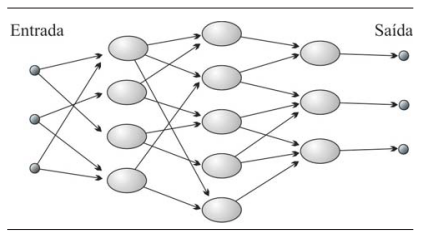
\includegraphics[width=.7\textwidth]{imagens/RNA.png}	}

	{\scriptsize 	Fonte: \cite[p.26]{ferneda_redes_2006}}
	\label{fig:rna}
\end{figure}

As  redes  neurais  artificiais  se  diferem  pelas  suas arquiteturas e pela forma como os pesos associados às conexões são ajustados durante o processo de aprendizado.	A arquitetura de uma rede neural restringe o tipo de problema no qual a rede poderá ser utilizada, e é definida pelo  número  de  camadas  (camada única  ou múltiplas camadas), pelo número de nós em cada camada, pelo tipo de conexão entre os nós (\textit{feedforward} ou \textit{feedback}) e por sua topologia. \cite[p. 46-49]{haykin_redes_2001}

O desenvolvimento de uma rede neural artificial consiste em determinar sua arquitetura, ou seja, os números de camadas e de neurônios em cada camada, bem como o ajuste dos pesos na fase conhecida como treinamento.\cite{hagan_neural_1996} \cite{haykin_redes_2001}

Uma das características mais importantes de uma rede neural artificial é a habilidade de aprender através de exemplos e fazer inferências sobre o que aprendeu, melhorando, assim, o seu desempenho. As RNA's utilizam um algoritmo de aprendizagem que serve, basicamente, para ajustar os pesos de suas conexões. \cite{haykin_redes_2001} \cite{ferneda_redes_2006} \cite{lima_ia_2016} \cite{Norvig2013}. 

Aqui também há, cf. explicitado na seção \ref{aprendizagem_maquina}, duas formas básicas de aprendizado, o supervisionado e o não-supervisionado.

\subsection{Redes do tipo Perceptron de múltiplas camadas}
As arquiteturas do tipo perceptron de múltiplas camadas (MLP) são os modelos de redes neurais mais utilizados e conhecidos. Elas, basicamente, consistem de uma camada de entrada e uma ou mais camadas intermediárias (ou ocultas) além, claro da camada de saída (uma ou mais unidades sensoriais - neurônios). \cite{haykin_redes_2001}.

Os sinais de entrada são propagados camada a camada pela rede em uma direção, ou seja, da entrada para a saída (\textit{feedfoward}). Esta arquitetura retrata uma generalização do perceptron. Portanto, segundo \citeonline[p. 26]{silva_redes_2016}, 
\begin{citacao}
	As redes Perceptron de múltiplas camadas (PMC) são caracterizadas pela presença de pelo menos uma camada intermediária (escondida) de neurônios, situada entre a camada de entrada e a respectiva camada neural de saída.
\end{citacao}

Desta forma, elas possibilitam elevadas possibilidades de aplicações em muitas áreas do conhecimento, entre as principais: aproximação universal de funções, reconhecimento de padrões, identificação e controle de processos, previsões de séries temporais, otimização de sistemas entre muitos outros. \cite{haykin_redes_2001}.

A \autoref{fig:pmc} ilustra uma rede do tipo perceptron de multicamadas. O treinamento deste tipo de rede é do tipo supervisionado e, geralmente, se utiliza um algoritmo muito popular chamado \textit{retropropagação} do erro (\textit{error backpropagation}). Este algoritmo é baseado numa regra de aprendizagem que “corrige” o erro durante o treinamento. \cite{haykin_redes_2001}

Substancialmente, o método de \textit{retropropagação} é constituído de duas etapas: uma fase de propagação do sinal no sentido tradicional (\textit{feedforward}) e uma de retropropagação do erro (\textit{backpropagation}) de todas as camadas e seus respectivos pesos. Na fase de ida, os vetores de dados e pesos são aplicados às unidades de entrada, e seu efeito se propaga pela rede, camada por camada \cite{hagan_neural_1996} \cite{haykin_redes_2001}.

Após isso, um conjunto de saídas é produzido como resposta da rede. Na retropropagação os pesos são ajustados de acordo com uma regra de correção de erro (normalmente uma função matemática com \ref{erro_absoluto}, \ref{erro_absoluto_medio}, \ref{erro_quadratico} e \ref{erro_quadratico_medio}, sendo esta última uma das mais utilizadas em muitas arquiteturas, na prática). \cite{haykin_redes_2001} \cite{hagan_neural_1996} \cite{yeung_neural_2004}

A resposta da rede em um instante é subtraída da saída desejada (\textit{target}) para produzir um valor de erro. Este valor de erro é propagado da saída para a entrada, camada a camada, de onde vem o nome “\textit{retropropagação} do erro”. Os pesos são, então, redefinidos de forma que a distância entre a resposta da rede e a resposta desejada seja reduzida (o erro seja minimizado). O processo é repetido diversas vezes até que uma tolerância global de erro seja assumida. Cada iteração é denominada época (\textit{epoch}). \cite{haykin_redes_2001} \cite{hagan_neural_1996} \cite{minsky_perceptrons:_1969}.

Uma arquitetura de um MLP (\textit{Multi-Layer Perceptron} - Perceptron Multicamadas), possui, portanto três propriedades distintas: a função de ativação, o número de camadas ocultas e forma das conexões (totalmente conectada ou não).

\begin{figure}[h!]
	\centering
	\caption{Rede Perceptron de multicamadas}
	\fbox{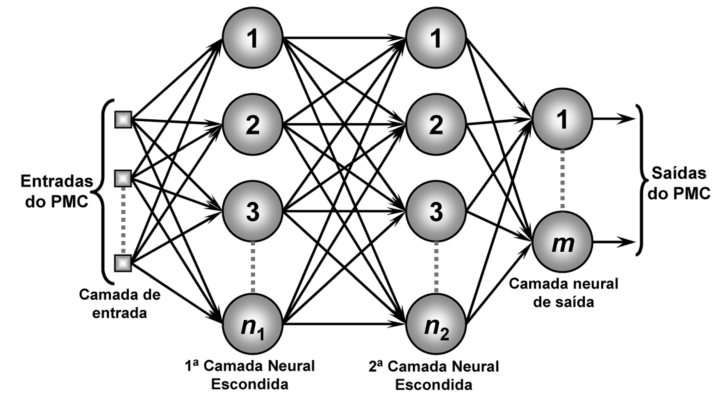
\includegraphics[width=.7\textwidth]{imagens/pmc.png}	}

	{\scriptsize 	Fonte: \citeonline[p. 92]{silva_redes_2016}}
	\label{fig:pmc}
\end{figure}

\subsection{Funções de ativação}\label{funcoes_ativacao}
Como visto na seção \ref{perceptron}, o modelo perceptron, lida bem com problemas linearmente separáveis, mas tem problemas ao lidar com problemas  não-lineares. \cite{haykin_redes_2001}. 

Para dar capacidade representativa às redes neurais artificiais, são essenciais as diferentes funções de ativação, pois só assim elas conseguirão lidar um componente de não-linearidade, como o são a maioria dos problemas práticos. \cite{hagan_neural_1996}.

Ao se introduzir ativações não-lineares, a superfície de custo da rede neural deixa de ser convexa fazendo com que a otimização se torne mais difícil. \cite{minsky_perceptrons:_1969} \cite{haykin_redes_2001}.

As principais funções de ativação, utilizadas na literatura ena prática, são, portanto:

\subsubsection{Função de ativação limiar}\label{ativacao:limiar}
Foi proposta na primeira definição de rede com neurônios artificiais \cite{rosenblatt_perceptron:_1958}. O modelo de neurônio usado por RosenBlatt foi o mesmo sugerido por \citeonline{mcculloch_logical_1943}. 

Neste modelo as saídas são binárias, ou seja, assumem, normalmente o valor 0 ou 1. A saída é 1 se o valor da entrada líquida for superior a um determinado valor chamado \textit{thereshold}. na maioria das vezes, esse valor é zero.

Matematicamente:
\begin{equation}\label{eq:limiar}
	y_k = y = f_i(a_i(t)) = \left \{ 
	\begin{matrix} 1\textrm{,} & \mbox{\textrm{se }}a_i(t) >= 0 \\
	0\mbox{\textrm{,}} & \mbox{\textrm{se }}a_i(t) < 0 \end{matrix} 
	\right.
\end{equation}

A \autoref{fig:binary_step} mostra o `funcionamento' da função de ativação limiar. Eventualmente podem ser utilizados os valores -1 e 1. Uma rede de camada simples que utiliza este tipo de ativação é o perceptron simples.

\begin{figure}[h!]
	\centering
	\caption{Função de ativação Limiar}
	\fbox{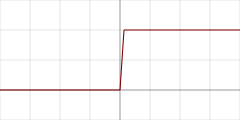
\includegraphics[width=.5\textwidth]{imagens/binary_step.png}	}

	{\scriptsize 	Fonte: Adaptado de \citeonline{haykin_redes_2001}}
	\label{fig:binary_step}
\end{figure}

\subsubsection{Função de ativação linear}\label{ativacao:linear}
A saída do neurônio, neste caso, é representada por uma função linear da forma descrita na \autoref{fig:ativacao_linear}. Redes que usam este tipo de função de ativação apresentam apenas uma camada de entrada e uma de saída. Possuem, portanto, uma série de representações quanto ao que são capazes de representar. \cite{lima_ia_2016}

\begin{figure}[h!]
	\centering
	\caption{Função de ativação Linear}
	\fbox{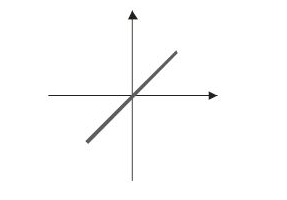
\includegraphics[width=.5\textwidth]{imagens/ativacao_linear.png}	}

	{\scriptsize 	Fonte: Adaptado de \citeonline{haykin_redes_2001}}
	\label{fig:ativacao_linear}
\end{figure}

\subsubsection{Funções de ativação semilineares}\label{ativacao_semilinear}
As funções de ativação mais usadas deste tipo são a função logística e a tangente hiperbólica. Elas são populares por conta de suas derivadas (que são necessárias nas etapas de treinamento, particularmente no \textit{Gradiente Descent} --- descida do gradiente) poderem ser expressas a partir das próprias funções.

Estas funções, tanto a logística (ou \textit{sigmoide}) e a tangente hiperbólica, respectivamente, podem ser expressas pelas equações \ref{eq:sigmoide_tanh} abaixo, onde $a$ representa a entrada líquida da unidade. \cite{haykin_redes_2001} \cite{lima_ia_2016} 

\begin{equation}\label{eq:sigmoide_tanh}
	f(a) = \frac{1}{1+ e^{(-2 \beta a)}} \qquad g(a) = tanh(\beta a)
\end{equation}

E as respectivas derivadas das funções \ref{eq:sigmoide_tanh} acima são dadas por:

\begin{equation}\label{derivadas_sigmoide_tanh}
	f'(a) = 2 \beta f(1-f) \qquad g'(a) = \beta (1-g^2)
\end{equation}

A \autoref{fig:ativacao_sigmoide} mostra o comportamento da função sigmoide e a \autoref{fig:tanh} mostra o da função tangente hiperbólica.

\begin{figure}[h!]
	\centering
	\caption{Função de ativação Logística (sigmoide)}
	\fbox{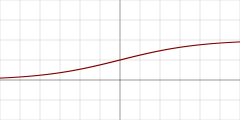
\includegraphics[width=.5\textwidth]{imagens/logistic.png}	}
	
	{\scriptsize 	Fonte: Adaptado de \citeonline{haykin_redes_2001}}
	\label{fig:ativacao_sigmoide}
\end{figure}

\begin{figure}[h!]
	\centering
	\caption{Função de ativação Tangente Hiperbólica}
	\fbox{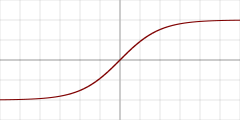
\includegraphics[width=.5\textwidth]{imagens/tanh.png}	}
	
	{\scriptsize 	Fonte: Adaptado de \citeonline{haykin_redes_2001}}
	\label{fig:tanh}
\end{figure}

\subsubsection{Função de ativação ReLu}
A função ReLU é a unidade linear retificada. É definida como, \citeonline{deep_learning_book_2019}:
\begin{equation}\label{relu}
	ReLU(x) = max(0,x)
\end{equation}
Sua derivada é dada por:
\begin{equation}\label{derivada_relu}
	ReLU'(x) = \left \{ \begin{matrix} 1, & \mbox{se }x > 0 \\ 
	0, & \mbox{\textrm{caso contrário}} \end{matrix} \right.
\end{equation}
Conforme, \citeonline{deep_learning_book_2019},
\begin{citacao}
	 ReLU é a função de ativação mais amplamente utilizada ao projetar redes neurais atualmente. Primeiramente, a função ReLU é não linear, o que significa que podemos facilmente copiar os erros para trás e ter várias camadas de neurônios ativados pela função ReLU.
\end{citacao}
Ainda, de acordo com \citeonline{deep_learning_book_2019}: 
\begin{citacao}
	A principal vantagem de usar a função ReLU sobre outras funções de ativação é que ela não ativa todos os neurônios ao mesmo tempo. [...] Se [...] a entrada for negativa, ela será convertida em zero e o neurônio não será ativado. Isso significa que, ao mesmo tempo, apenas alguns neurônios são ativados, tornando a rede esparsa e eficiente e fácil para a computação.
\end{citacao}

A \autoref{fig:relu} demonstra o comportamento da função de ativação ReLu em função da entrada

\begin{figure}[h!]
	\centering
	\caption{Função de ativação ReLu (sigmoide)}
	\fbox{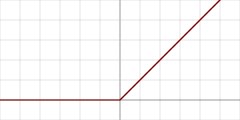
\includegraphics[width=.5\textwidth]{imagens/relu.png}	}
	
	{\scriptsize 	Fonte: Adaptado de \citeonline{haykin_redes_2001}}
	\label{fig:relu}
\end{figure}

Redes com a função ReLU são mais fáceis de otimizar porque a função é parecida com a função identidade. A única diferença é que a ReLU produz zero em metade de seu domínio. \cite{hagan_neural_1996}.

\section{Otimização}\label{otimização}
Redes Neurais tem uma etapa iterativa em que os pesos são ajustados e se pode realizar otimizações para melhorar o erro e incrementar o modelo. \cite{haykin_redes_2001}.

Normalmente, o fluxo de treinamento se resume nos seguintes passos iterativos:
\begin{enumerate}\label{fluxo_treinamento}
	\item Opera a entrada na rede
	\item Cálculo da função de perda (\textit{loss function}) ou outra função de cálculo de erro
	\item Cálculo do gradiente
	\item Atualização dos pesos
	\item Volta para o passo 1
\end{enumerate}

Este processo é repetido até que um hiperparâmetro de tolerância seja alcançado para o cálculo dos erros mediante a \textit{loss function} ou outra função de cálculo do erro.

O cálculo do gradiente descrito anteriormente diz respeito, cf. \cite{deep_learning_book_2019} a um dos mais usados algoritmos para otimizar a tarefa de aprendizagem dos pesos de uma rede neural.

De acordo com \citeonline{deep_learning_book_2019}: 
\begin{citacao}
	A Descida do Gradiente é uma ferramenta padrão para otimizar funções complexas iterativamente dentro de um programa de computador. Seu objetivo é: dada alguma função arbitrária, encontrar um mínimo. Para alguns pequenos subconjuntos de funções – aqueles que são convexos – há apenas um único \textit{minimum} que também acontece de ser global. Para as funções mais realistas, pode haver muitos mínimos, então a maioria dos mínimos são locais.[... É preciso] que a otimização encontre o “melhor” \textit{minimum} e não fique preso em mínimos sub-otimistas (um problema comum durante o treinamento do algoritmo).
\end{citacao}

O algoritmo consiste basicamente de subtrair o valor do gradiente $\nabla f$ dos pesos $w$ da rede, assim:
\begin{equation}\label{gradiente}
	w_i = w_i - \alpha \times \nabla f_i
\end{equation}
Sendo $\alpha$ o multiplicador que nos permite controlar o tamanho do passo de otimização.  $\nabla f$ é a derivada da função de ativação no ponto específico. $\alpha$ é um hiperparâmetro conhecido como taxa de aprendizado e repreenta a \textit{velocidade} em que a rede neural ``aprende'' os melhores pesos para o problema específico. \cite{haykin_redes_2001}.

Uma iteração consiste em um passo de otimização como o descrito em \ref{fluxo_treinamento} e corresponde a uma ligação sináptica de \textit{forward} na rede e uma de \textit{backpropagation}. Isto constitui uma \textbf{\underline{época}}. Normalmente, muitas épocas são necessárias, visto que o aprendizado em uma rede neural é, geralmente, lento para que a otimização evite os mínimos locais.

\section{SVM - Support Vector Machines}\label{SVM}
Segundo \citeonline{cortes_svm_1995}, o algoritmo SVM (\textit{Support Vector Machines}) é um dos mais efetivos para a tarefa de classificação.

Cf. \citeonline{goldschmidt2005},
\begin{quotation}
	No algoritmo SVM, o conjunto de dados de entrada é utilizado para construir uma \textit{função de decisão} $f(x)$, tal que:
	
		\begin{equation}
			\begin{matrix}
				Se & f(x_i) \ge 0, & \textrm{então} &  y_i = 1   \\
				Se & f(x_i) < 0,   & \textrm{então} &  y_i = -1   
			\end{matrix}
		\end{equation}

	O algoritmo SVM constrói os denominados classificadores lineares, que separam o conjunto de dados por meio de um \textit{hiperplano} que é a generalização do conceito de \textit{plano} para dimensões maiores que três.	
\end{quotation}

Assim, SVM, cf. \citeonline[p. 45]{aprenda_mineracao_fernando_amaral16} ``são um algoritmo de classificação que maximizam as margens entre instâncias mais próximas, dessa forma, é criado um vetor otimizado que é então utilizado para classificar novas instâncias''.

Conforme se vê na \autoref{fig:svm}, os dois vetores \textit{não pontilhados} são as margens otimizadas. As instâncias por onde as margens otimizadas passam são os vetores de suporte. O vetor pontilhado é a referência para classificar novas instâncias. Assim, a nova instância, na figura \ref{fig:svm} é classificada como triângulo.

\begin{figure}[h!]
	\centering
	\caption{Vetores de Suporte}
	\fbox{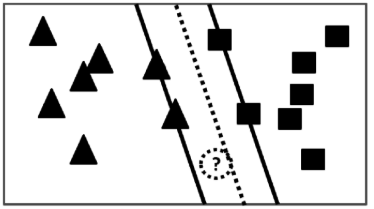
\includegraphics[width=.7\textwidth]{imagens/vetores_de_suporte.png}	}
	
	\label{fig:svm}
	{\scriptsize 	Fonte: \cite[p. 45]{aprenda_mineracao_fernando_amaral16}}
\end{figure}

Seguindo o estudo de \citeonline{mukkamala_intrusion_2002} há duas razões principais que levaram os autores do artigo citado de usarem SVMs para detecção de intrusão:o primeiro é a velocidade já que a performance é prioritariamente uma das características mais importantes para sistemas de detecção de intrusos. 

A segunda razão é a escalabilidade, pois, cf. os autores, SVMs são relativamente indiferentes ao número de \textit{data points} e a complexidade da classificação não depende da dimensionalidade do espaço de características. Dependendo da aplicação, ainda conforme os autores, uma vez que os dados estão classificados em duas classes, um algoritmo de otimização adequado pode ser usado, se necessário,  para identificação de mais características.

Neste trabalho, também foi usado, com boa eficácia (cf. se vê na seção \ref{resultados}) o algoritmo SVM.

\section{Trabalhos Relacionados}\label{trabalhos_relacionados}
Esta seção expõe alguns dos principais trabalhos encontrados na literatura que estão, de alguma forma, relacionados a esta dissertação. Foram estudadas e analisadas obras acerca das políticas de segurança da informação, abordando a detecção de conflitos em diversos contextos como identificação e resolução de conflitos aéreos, rodoviários e de \textit{normas} além de trabalhos sobre mineração de dados e técnicas de aprendizagem de máquina tanto em conjunturas distintas como regressão e classificação quanto para localização e solução de conflitos, no caso específico das políticas de segurança, principalmente sendo usadas em registros de patentes americanas fechadas --- o que, de certa forma, evidencia o quanto este tema está na vanguarda.

Por exemplo, \citeonline{guerrero-higueras_detection_2018} aborda um método para construir modelos de \textit{aprendizagem de máquina} com o objetivo de detectar ataques cibernéticos em RTLSs (\textit{Real Time Location Systems} - sistemas de localização em tempo real ) em um ambiente de cibersegurança para sistemas robóticos usando técnicas de \textit{Machine Learning}.  O artigo mostra que os ciberataques nos sistemas de localização em tempo real para sistemas robóticos podem ser detectados por um sistema criado usando o aprendizado supervisionado. Além disso, mostra que alguns tipos de ciberataques em sistemas de localização em tempo real, especificamente negação de serviço e falsificação(\textit{DoS} e \textit{Spoofing}), podem ser detectados por um sistema construído usando técnicas de aprendizado de máquina. Oito classificadores e algoritmos preditores conhecidos foram avaliados neste artigo e a análise de validação cruzada mostrou que os classificadores MLP (\textit{Multi Layer Perceptron}) funcionam melhor que os outros obtendo maior acurácia e menor erro, sendo também o modelo com menor \textit{overfitting} e maior \textit{sensibilidade}\footnote{Sensibilidade é a proporção de verdadeiros positivos: a capacidade do sistema em predizer corretamente a condição para casos que realmente a têm - É também conhecida como \textit{\textbf{Recall}}.}. Este artigo inspirou a hipótese desta dissertação.

Já \cite{bui_efficient_2019} versa acerca de mineração de dados em políticas de controle de acesso, especificamente do modelo ReBAC (\textit{Relationship-Based Access Control} - controle de acesso baseado em \textit{relacionamento}), mas não foca na detecção de conflitos entre as políticas, e sim, na propagação de seus relacionamentos na criação de novas políticas. No artigo, os algoritmos de mineração de política do ReBAC propostos puderam reduzir significativamente o custo da migração dos sistemas de controle de acesso legados para o ReBAC, automatizando parcialmente o desenvolvimento de uma nova política do ReBAC.

O trabalho de \cite{lupu_conflicts_1999} discorre sobre conflitos no gerenciamento de sistemas distribuídos com base em políticas de controle de acesso. O artigo analisa os conflitos de políticas, concentrando-se nos problemas de detecção e resolução dos mesmos. Discute-se, no artigo, os vários relacionamentos de precedência que podem ser estabelecidos entre as políticas e é apresentado uma ferramenta de análise de conflitos que faz parte de uma estrutura de gerenciamento baseada em funções, porém, sem usar mineração de dados ou aprendizagem de máquina.

O artigo de \cite{koch_conflict_2002}, estudou,  usando como base grafos, a detecção e resolução de conflitos nas especificações das políticas de controle de acesso. Os autores usam propriedades formais de transformações de grafos para detectar sistematicamente inconsistências entre restrições, entre regras e entre uma regra e uma restrição em políticas de controle de acesso e estabelecer as bases para suas resoluções,  porém, também não usando mineração de dados ou aprendizagem de máquina.

Já \cite{neri_conflict_2012}, abordaram a detecção de conflitos em políticas de segurança usando as tecnologias da Web Semântica. É mostrado, no artigo, como as ferramentas fornecidas pelas tecnologias de gerenciamento de Web Semântica e Ontologia oferecem uma base adequada para a realização de técnicas capazes de suportar a análise de conflitos nas políticas de segurança. Com base no uso dessas técnicas, é proposto no artigo, uma solução para duas variantes diferentes de análise de conflitos: (a) incompatibilidade de políticas e (b) satisfação de separação de tarefas. 

\cite{obaidat_multilayer_1994} aborda um sistema de rede neural multicamadas para segurança de acesso a computadores com o objetivo de identificar usuários do mesmo. Os vetores de entrada foram compostos pelos intervalos de tempo entre pressionamentos de teclas sucessivos criados pelos usuários ao digitar uma sequência conhecida de caracteres. Usando aprendizado supervisionado, cada vetor de entrada foi classificado em uma das várias classes, identificando assim o usuário que digitou a sequência de caracteres. Neste artigo, uma precisão máxima de classificação de 97,5\% foi alcançada usando um classificador de padrões baseado em rede neural multicamadas \textit{feedforward} treinada usando \textit{backpropagation}, o algoritmo de retropropagação. Essa abordagem visa melhorar a segurança do acesso ao computador. Este artigo trouxe importantes contribuições para esta dissertação na maneira de construir a arquitetura da rede neural e também no ajuste dos hiperparâmetros.

O trabalho de \cite{christodoulou_collision_2008} aborda a detecção de conflitos sobre a ótica da prevenção de colisões no voo livre de aeronaves comerciais usando redes neurais com exemplos preparados por meio de programação não linear. 

Na mesma linha, o artigo de \cite{mukkamala_intrusion_2002} estuda a detecção de invasões usando redes neurais e máquinas de vetores de suporte e a ideia central é descobrir padrões úteis ou características que descrevam o comportamento intrusivo de um usuário em um sistema e os autores usam este conjunto de características para construir classificadores que puderam reconhecer anomalias e intrusões conhecidas em tempo real. É usado um conjunto de dados de referência de uma competição de KDD (\textit{Knowledge Discovery in Databases} --- Descoberta de Conhecimento em Bases de Dados) projetada pela DARPA (Defense Advanced Research Projects Agency), e é demonstrado que classificadores eficientes e precisos podem ser construídos para detectar invasões. Ao final é comparado o desempenho de redes neurais e máquinas de vetores de suporte para a detecção de intrusões. Nesta dissertação, baseando-se neste artigo de \cite{mukkamala_intrusion_2002} também serão avaliados os desempenhos de redes neurais e máquinas de vetores de suporte, mas para detecção de conflitos em políticas.

\cite{thenmozhi_multi-lingual_2018} apresenta uma discussão sobre a criação de perfis de autores multilíngues em mensagens SMS usando a abordagem de aprendizado de máquina com seleção estatística de recursos que mostra, de forma didática, formas de tratar os hiperparâmetros de uma rede neural usando uma abordagem estatística. Este artigo forneceu suporte teórico para o sucessivo e repetitivo trabalho de ajuste dos hiperparâmetros tanto das redes neurais construídas nesta dissertação quanto dos outros classificadores.

Já o trabalho de \cite{jin_development_2002} aborda o desenvolvimento e uso de uma rede neural probabilística construtiva (\textbf{CPNN} - \textit{Constructive Probabilistic Neural Network}) na detecção de incidentes em rodovias, incluindo a construção e adaptação dos modelos. Esta CPNN foi estruturada com base no modelo Gaussiano de mistura e treinada por um algoritmo de ajuste dinâmico de decaimento (para correção dos erros). Os incidentes em rodovias, como colisões de veículos, podem ser extrapolados para um modelo de conflito entre agentes de um sistema. O modelo foi treinado e avaliado sobre um banco de dados de incidentes simulados em Singapura e adaptado para a rodovia I-880 na Califórnia sendo então investigada em ambientes on-line e off-line. Este artigo citado compara o desempenho do modelo CPNN e um modelo de rede neural probabilística básica (BPNN - Basic Probabilistic Neural Network).

O artigo de \cite{debar_neural_1992} estuda um componente de rede neural para um sistema de detecção de intrusão. O modelo \textit{aprende} os hábitos que um usuário tem enquanto trabalha com o computador e emite avisos quando o comportamento atual não é consistente com os padrões \textit{aprendidos} anteriormente. O modelo de de rede neural  é usado para modelar o comportamento do usuário como uma característica componente para o sistema de detecção de intrusão.

O artigo de \cite{chen_flight_2011} trabalha com a identificação e a resolução de conflitos de voo com base em redes neurais. No artigo, o autor considera os problemas de detecção e resolução de conflitos no gerenciamento de tráfego aéreo (ATM - \textit{Air Traffic Management}) sob a perspectiva da geometria computacional e fornece algoritmos para resolver esses problemas além de propor um método que pode rotear várias aeronaves, sem conflitos, através do espaço aéreo, usando um esquema de roteamento priorizado no espaço-tempo através do uso de conjunto de soluções ótimas por meio de uma rede neural.

Importante citar a patente assinada pelos inventores \cite{ahuja_54_nodate}, "Sistema e método para mineração de dados e gerenciamento de políticas de segurança", tendo a  McAfee como cessionária, que propõe um método para mineração de dados automatizada e criação de políticas de segurança em redes e sistemas.

Todos estes trabalhos foram base para o estudo, amadurecimento bibliográfico e aprofundamento teórico sobre o problema e as soluções propostas neste trabalho, principalmente aqueles relacionados a intrusões, detecção de conflitos aéreos e as soluções baseadas em aprendizado de máquina, com ênfase nas redes neurais e nas máquinas de vetores de suporte (SVM)  pois não só serviram de inspiração como ofereceram estímulo para que as técnicas pudessem ser extrapoladas para o uso na detecção de conflitos em políticas, tema desta dissertação.

\cite{sarkis2017}, \cite{eduardo2017} e \cite{sarkis:artigo:2016} são os trabalhos-base no estudo da detecção de conflitos, da determinação do modelo das políticas utilizadas e analisadas além de serem a fonte de algumas das principais definições empregadas neste trabalho. 

\cite{eduardo2017} estuda a verificação de conflitos entre múltiplas normas em sistemas multiagentes (SMA). As normas, nesta tese, são semelhantes às políticas, inclusive em suas definições, mas restritas a um contexto de agentes autônomos. Para a resolução de conflitos, o autor usa uma estratégia de aplicação de filtros para suavizar o custo computacional e utiliza transformação deôntica para análise de diversas normas ao mesmo tempo.

As hipóteses e problemas estudados por esta proposta de dissertação complementam o estudo  de \citeonline{sarkis2017} e são, em parte, uma adição do mesmo usando algoritmos de mineração de dados e aprendizagem de máquina.

\chapter{Experimentos/Resultados}\label{resultados}
Neste capítulo serão descritas as 3 abordagens diferentes que foram utilizadas e em cada uma delas, os principais algoritmos de classificação que foram utilizados. A primeira parte dos experimentos focaram em determinar quais os classificadores apresentaram melhor acurácia para a resolução do problema descrito em \ref{problema}. Em seguida, os dois que apresentaram melhor acurácia foram utilizados nos experimentos subsequentes.

\section{Forma geral dos experimentos}\label{forma_geral_experimentos}
A forma geral de como a estrutura dos experimentos foram realizados para o problema proposto em \ref{problema} é a seguinte:
\begin{enumerate}
	\item Definição do problema;
	\item Coleta de dados;
	\item Pré-processamento dos dados;
	\item Engenharia e seleção de atributos;
	\item Modelagem: definição, configuração e arquitetura da rede (ou modelagem dos hiperparâmetros do SVM);
	\item Treinamento (Aprendizagem da rede neural e do SVM);
	\item Testes e validação do modelo;
		\item Avaliação e ajuste do modelo;
	\item Apresentação dos resultados;
\end{enumerate}

Este modelo de método experimental foi adaptado daqueles propostos em \cite{lima_ia_2016}, \cite{silva_redes_2016} e \cite{haykin_redes_2001}. Cada seção posterior seguirá o definido nesta \autoref{forma_geral_experimentos} e seguirá os passos descritos nesta seção.

\section{Base de dados, pré-processamento e recursos computacionais}\label{base_dados}
\subsection{Experimentos iniciais - arquivo com 68 políticas}
Para os experimentos iniciais, um arquivo de políticas foi gerado randomicamente a partir do proposto em \cite{sarkis2017} e, de acordo com o exposto na seção \ref{modelo_politica_utilizada}. O arquivo gerado possui, inicialmente, cerca de 68 políticas nomeadas (constituindo a \textit{fase de seleção}\footnote{cf. seção \ref{mineracao_dados} deste trabalho.} da Mineração de Dados) e da fase coleta de dado do método proposto anteriormente. 

Este arquivo foi usado nos testes preliminares da hipótese descrita na seção \ref{hipótese} deste trabalho. Para este problema da detecção de conflitos diretos serão usadas técnicas de aprendizagem supervisionada. 

Para tanto, ao arquivo com as políticas, no pré-processamento foi acrescentada uma coluna rotulando os conflitos da seguinte forma: \textbf{1}: \textit{conflito direto} e \textbf{0}: \textit{sem conflito}. Esta estratégia é a mesma utilizada no trabalho de \cite{davy_application_2008} onde ele usa um modelo de matriz de controle de acesso usando operações lógicas \texttt{AND} e \texttt{OR} para identificação de conflitos.

A figura \ref{fig:aspecto_arquivo} demonstra o aspecto do arquivo das políticas geradas paraos experimentos deste trabalho. Na imagem, pode-se notar a classe (coluna) criada para guiar o aprendizado supervisionado dos algoritmos utilizados no estudo.

\begin{figure}[h!]
	\centering
	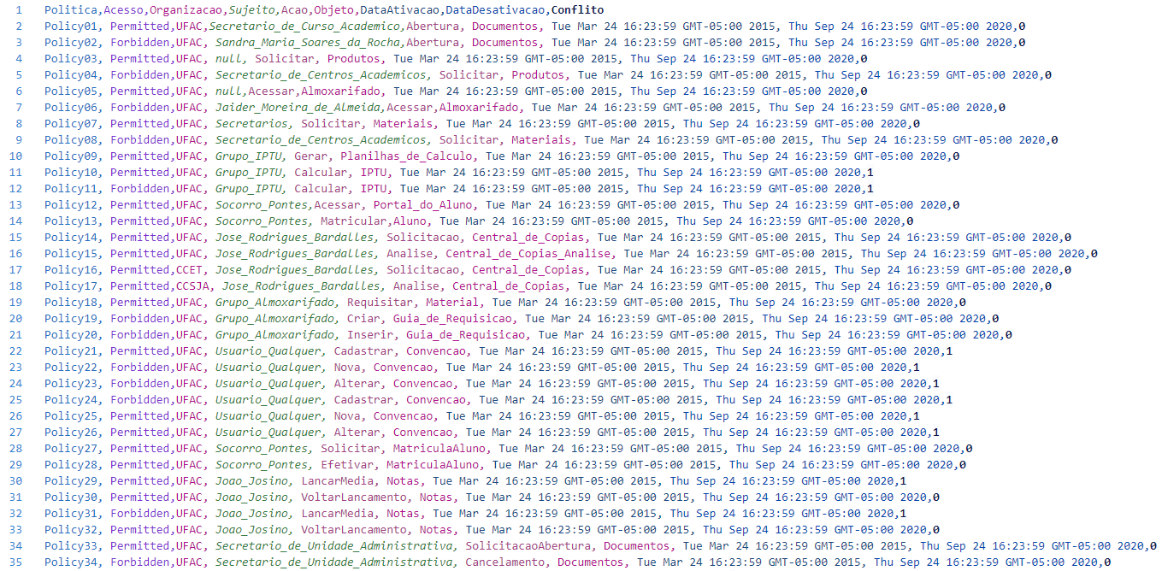
\includegraphics[width=.8\textwidth]{imagens/aspecto_arquivo_politicas.png}	
	\caption{Aspecto do arquivo das políticas geradas para os experimentos}
	\label{fig:aspecto_arquivo}
	{\scriptsize Fonte: compilação do autor}
\end{figure}

\subsection{Recursos computacionais}
Dois \textbf{ambientes computacionais} foram utilizados para as tarefas de mineração: um \textbf{notebook}  Intel Core i5 vPro-8350U (8ª Geração de 64 bits com 1.70GHz e 8 GB de RAM, com SSD de 256 GB rodando Windows 10 Pro.
 
O outro ambiente foi um \textbf{Desktop} Intel Core i7 vPro-6700 de 8ª geração de 64 bits com 3.40 Ghz e 20 GB de RAM, com HD de 1 TB rodando o Windows 10 Pro.

\subsubsection{Pré-processamento}
Ainda na fase de \textit{pré-processamento}, a coluna 9 (Conflito) foi transformada do tipo de dado \textit{Numérico para Nominal}. Para isso foi usado o softwate WEKA (descrito em \cite{eibe2016}) aplicado o filtro \textit{NumericToNominal} do software. Além disso, tanto o primeiro atributo quanto a data foram removidos, pois, dentro do escopo estudado neste trabalho, eles não influenciariam nos resultados finais.

\subsubsection{Resultados - Arquivo com 68 políticas}
Logo após, mais de 30 experimentos foram realizados de forma preliminar no \textit{dataset} envolvendo os diversos algoritmos e muitos parâmetros alterados (a maioria com pequena ou nenhuma variação) para se chegar às técnicas finais que foram utilizadas nos posteriores experimentos e que serão explicitadas a seguir.

Utilizando-se a ferramenta WEKA (\cite{eibe2016}) para as últimas fases do KDD (Mineração de Dados), foram utilizados alguns algoritmos de classificação que segundo \cite{wu2007} são alguns dos mais utilizados na Mineração de Dados. Para avaliar o desempenho definiu-se o método \textit{cross-validatio}n com 10 folds. Em seguida suas acurácias foram comparadas.

A tabela \ref{tab:acuracias} mostra o resultado destes experimentos:

\begin{table}[h!]
	\centering
	\caption{Acurácia dos classificadores}
	\label{tab:acuracias}
	\vspace{0.3cm}
	\begin{tabular}{p{6cm}c}
		\hline\\
		Classificador/Algoritmo& Acurácia  \\[10pt] 
		\hline
		Multi Layer Perceptron & 0.9705    \\
		SVM kernel linear~     & 0.9705    \\
		Random Forest~		   & 0.9542	   \\
		J48                    & 0.9411    \\
		K* (K-star)            & 0.9411    \\
		Trees LMT              & 0.9117    \\
		IBk (KNN, com k =1)~   & 0.8970    \\
		JRip                   & 0.8970    \\		
		Nayve Bayes            & 0.8674    \\
		Random Tree            & 0.7794    \\
		\hline
	\end{tabular}
	\\[6pt]	\centering {\footnotesize Fonte: Elaborada pelo autor mediante experimentos}	
\end{table}

As figuras \ref{fig:saida_svm} e \ref{fig:saida_multilayerperceptron} mostram os resultados das classificações do arquivo de políticas usando, respectivamente, os classificadores/algoritmos: \textit{SVM} e o \textit{MultiLayer Perceptron} (que foram os principais citados nos trabalhos relacionados, cf. descrito na seção \ref{trabalhos_relacionados}). Cf. mostrado na tabela \ref{tab:acuracias}, os classificadores SVM e MultiLayerPerceptron ficaram empatados em relação à acurácia. Nos experimentos posteriores, apenas os dois foram considerados.
\begin{figure}[h!]
	\centering
	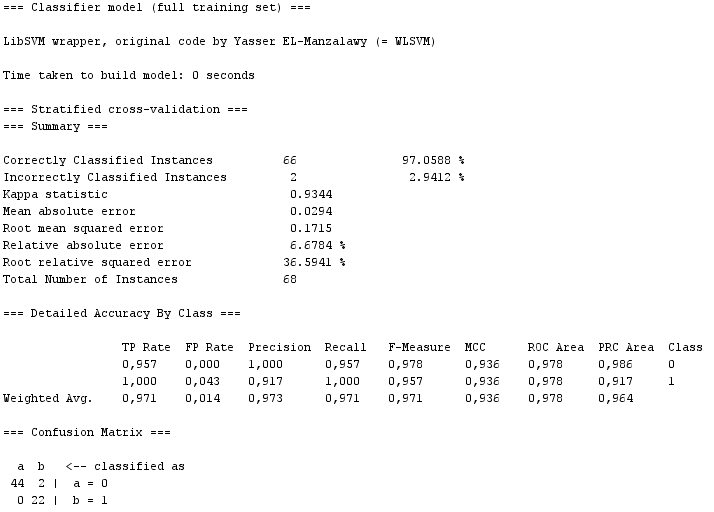
\includegraphics[width=.7\textwidth]{imagens/svm-resultados.png}	
	\caption{Saída do software WEKA. Classificador: SVM}
	\label{fig:saida_svm}
	{\scriptsize Fonte: compilação do autor}
\end{figure}
\begin{figure}[h!]
	\centering
	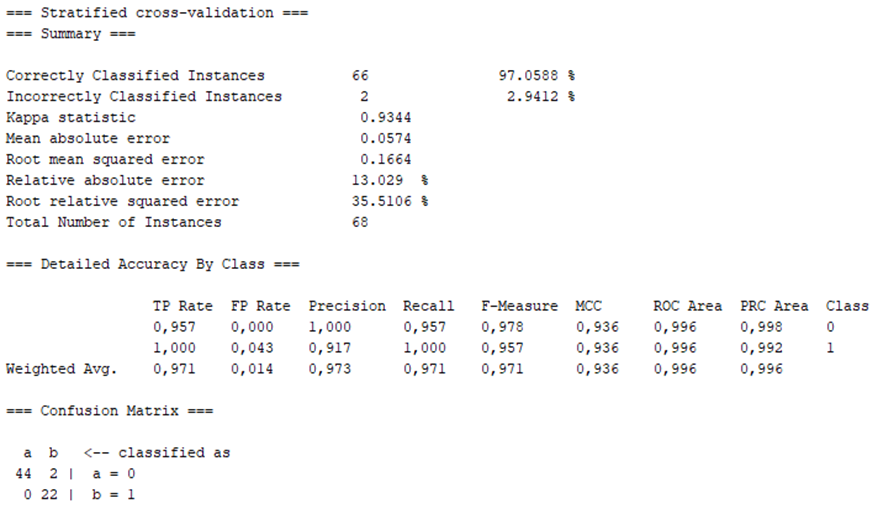
\includegraphics[width=.7\textwidth]{imagens/multilayerperceptron-resultados.png}
	\caption{Saída do software WEKA. Classificador: \textit{MultiLayer Perceptron}}
	\label{fig:saida_multilayerperceptron}
	{\scriptsize Fonte: compilação do autor}
\end{figure}

Assim, com uma acurácia de 97,05\% na classificação dos conflitos diretos, tanto o algoritmo Multilayer Perceptron (que implementa uma rede neural sigmoide multicamadas) quanto o SVM tiveram a maior acurácia, com 95,7\% de \textit{TP rate}(taxa de \textit{True Positives} ou verdadeiros positivos) para a classe 0 (não há conflito) e, somente, 4,3\% de \textit{FP rate}(taxa de Falsos Positivos) para a classe 1 (quando há conflito direto). Nos experimentos realizados (assim como se esperava inicialmente na hipótese deste trabalho --- baseado em evidências da literatura), estes modelos algorítmicos foram os mais eficientes para a detecção de conflitos diretos.

A interface visual do WEKA é excelente para observar o comportamento inicial dos algoritmos, mas para as arquiteturas de redes neurais e seus diversos parâmetros, configurações e quantidade de camadas ocultas, de neurônios nas camadas ocultas, entre outras configurações levaram a outros experimentos. Para isso e com o objetivo de evitar o overfitting (como explicado na seção \ref{medidas_avaliacao} novos procedimentos e ferramentas foram adotados).

\section{Outros experimentos - arquivos com 139 e 281 políticas}
Foi gerado, então, dois novos arquivos de políticas foram gerados randomicamente também a partir do proposto em \cite{sarkis2017} e, ainda conforme o exposto na seção \ref{modelo_politica_utilizada}. Os arquivos gerados agora, possui, 139  e 281 políticas nomeadas.

Os mesmos filtros anteriores foram aplicados e os resultados para os algoritmos (ainda usando a ferramenta Weka) foram os seguintes:

Para o MultiLayer Perceptron, a tabela \ref{tab:MLP_acuracia} mostra como as acurácias ficaram com os arquivos com quantidades diferentes de políticas.

\begin{table}[h!]
	\centering
	\caption{Acurácia do MLP}
	\label{tab:MLP_acuracia}
	\vspace{0.3cm}
	\begin{tabular}{p{6cm}c}
		\hline\\
		Qtd. de Políticas	& Acurácia  \\[10pt] 
		\hline
		68 					& 97.05    	\\
		139			     	& 98.73     \\
		281					& 99.28		\\
		\hline
	\end{tabular}
	\\[6pt]	\centering {\footnotesize Fonte: Elaborada pelo autor mediante experimentos}	
\end{table}

Para o classificador SVM, a tabela \ref{tab:SVM_acuracia} mostra como as acurácias ficaram com os arquivos com quantidades diferentes de políticas.

\begin{table}[h!]
	\centering
	\caption{Acurácia do SVM}
	\label{tab:SVM_acuracia}
	\vspace{0.3cm}
	\begin{tabular}{p{6cm}c}
		\hline\\
		Qtd. de Políticas	& Acurácia  \\[10pt] 
		\hline
		68 					& 97.05    	\\
		139			     	& 96.40     \\
		281					& 99.28		\\
		\hline
	\end{tabular}
	\\[6pt]	\centering {\footnotesize Fonte: Elaborada pelo autor mediante experimentos}	
\end{table}

Mesmo com uma leve queda na acurácia do SVM no arquivo de 139 políticas, percebe-se que, quanto maior o número de políticas, maior é a acurácia do classificador e melhor é a classificação.

\subsection{Experimentos com Pandas, NumPy e sklearn}
Entretanto, outros experimentos foram realizados utilizando as bibliotecas Pandas, NumPy e sklearn e o Notebook Jupyter. O notebook criado demonstra o treinamento de uma rede neural Rede Neural Multicamadas usando o classificador \texttt{\textbf{MLPClassifier}} da biblioteca \texttt{\textbf{sklearn}}

No arquivo, é demonstrado os experimentos na construção de uma arquitetura de uma rede neural com a estratégia de testes \textit{holdout} sendo a divisão da base (split) em atributos previsores e classe com cerca de 75\% da base sendo usada para treinamento da rede e 25\% para teste.

Há também um pré-processamento importante focado em um tratamento dos dados categóricos do \textit{dataset} e sua conversão para dados numéricos e divisão da base original em dois conjuntos de dados (previsores e classe).

Todos os atributos categóricos do dataset de políticas (o maior, com 281 instâncias) foram transformados para numéricos sendo um dicionário de dados construído.

Os passos foram os seguintes:

Primeiramente a base foi importada da seguinte forma, como demonstrado na figura \ref{fig:base-head} mostrando o aspecto inicial do dataset.

\begin{figure}[h!]
	\centering
	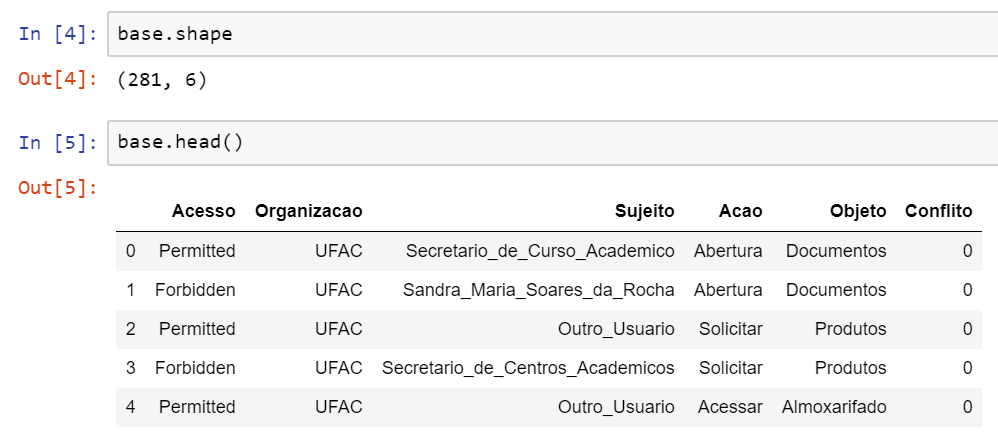
\includegraphics[width=.6\textwidth]{imagens/notebook-base1.png}
	\caption{Aspecto do dataset importado}
	\label{fig:base-head}
	{\scriptsize Fonte: compilação do autor}
\end{figure}

A partir daí, foram selecionados da base todas as linhas dos atributos do \textit{dataset} que estavam com os tipos \textit{object}. Foram procurados valores nulos e não foram encontrados. Foi usada uma técnica que transforma um atributo categórigo com $k$ valores em uma representação numérica com valores inteiros para cada $k$ valor. Há vantagens e desvantagens nessa abordagem. Elas estão discutidas em detalhes em \cite{sarkar_2017}.

A figura \ref{fig:dic-coluna1} demonstra como este procedimento foi realizado para o atributo que representa o acesso (Permitido, Proibido e Obrigatório).

\begin{figure}[h!]
	\centering
	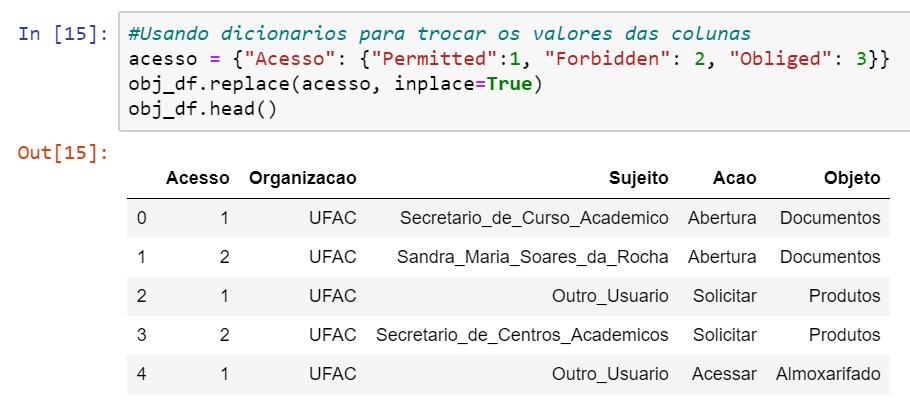
\includegraphics[width=.6\textwidth]{imagens/notebook-base2.png}
	\caption{Engenharia de atributos - dados categóricos textuais}
	\label{fig:dic-coluna1}
	{\scriptsize Fonte: compilação do autor}
\end{figure}

Em seguida a base foi dividida em atributos previsores e a classe. Os previsores são as colunas que representam a política em si e a classe é a representação binária do conflito.

O aspecto dos atributos previsores ficou como o mostrado na imagem \ref{fig:previsores}.

\begin{figure}[h!]
	\centering
	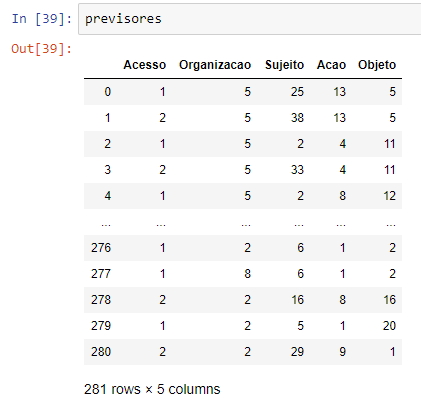
\includegraphics[width=.6\textwidth]{imagens/previsores.png}
	\caption{Aspecto dos atributos previsores}
	\label{fig:previsores}
	{\scriptsize Fonte: compilação do autor}
\end{figure}

Já a classe ficou com o aspecto da figura \ref{fig:classe}

\begin{figure}[h!]
	\centering
	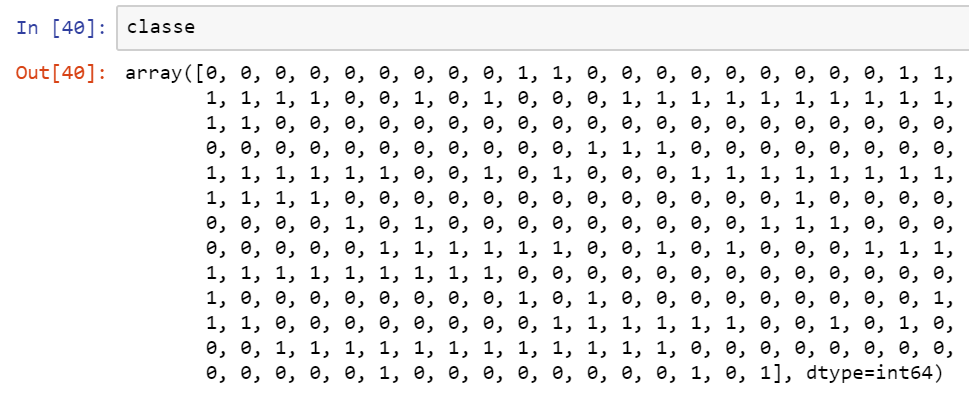
\includegraphics[width=.6\textwidth]{imagens/classe.png}
	\caption{Aspecto do atributo classe}
	\label{fig:classe}
	{\scriptsize Fonte: compilação do autor}
\end{figure}

Em seguida os atributos foram transformados usando padronização para manter as variáveis na mesma ordem de grandeza. Na padronização, a média se iguala a 0 e o desvio-padrão se mantém em 1. A fórmula da padronização é a seguinte:
\begin{equation}\label{padronizacao}
	z = \frac{x - \mu}{\sigma}
\end{equation}
onde $\mu$ é a média aritmética e $\sigma$ é o desvio-padrão dos dados. Como todos os dados estão agora em formato numérico, é um passo importante.

O código para a padronização foi o abaixo:
\begin{verbatim} 
from sklearn.preprocessing import StandardScaler
scaler = StandardScaler()
previsores_transformados = scaler.fit_transform(previsores)
\end{verbatim}
Assim os dados foram padronizados e ficaram na mesma escala. Foi gerado um novo conjunto de dados de treinamento com 75\% do \textit{dataset} (sendo escolhidos randomicamente). Deixando, assim, 25\% da base para validação.

Logo em seguida, um modelo de Multi-Layer Perceptron foi criado usando o classificador \texttt{\textbf{MLPClassifier}} da biblioteca \texttt{\textbf{sklearn}} com os seguintes hiperparâmetros: 
\begin{itemize}
	\item \texttt{$max\textunderscore iter=10000$,}
	\item \texttt{$tol = 0.0000010$,}
	\item \texttt{$solver = 'adam'$,}
	\item \texttt{$hidden\textunderscore layer\textunderscore sizes=(100)$ ,}
	\item \texttt{$shuffle=False$,}
	\item \texttt{$activation='relu'$}
\end{itemize}

Onde, respectivamente estão configuradas, o número máximo de épocas de treinamento (10000), a tolerância (0.0000010), a função de otimização de peso (`adam' refere-se a um otimizador estocástico baseado em gradiente descendente), a quantidade de neurônios na única camada oculta, se as amostras devem ser embaralhadas em cada iteração (marcado como falso) e a função de ativação da camada oculta (função de ativação ReLU).

A figura \ref{fig:mlp_classifier} mostra o código no notebook e as iterações finais onde o classificador indica que a função de perda no treinamento não melhorou mais do que a tolerância, $tol = 0,000001$ por 10 épocas consecutivas e, portanto, ele encerrou as iterações.

\begin{figure}[h!]
	\centering
	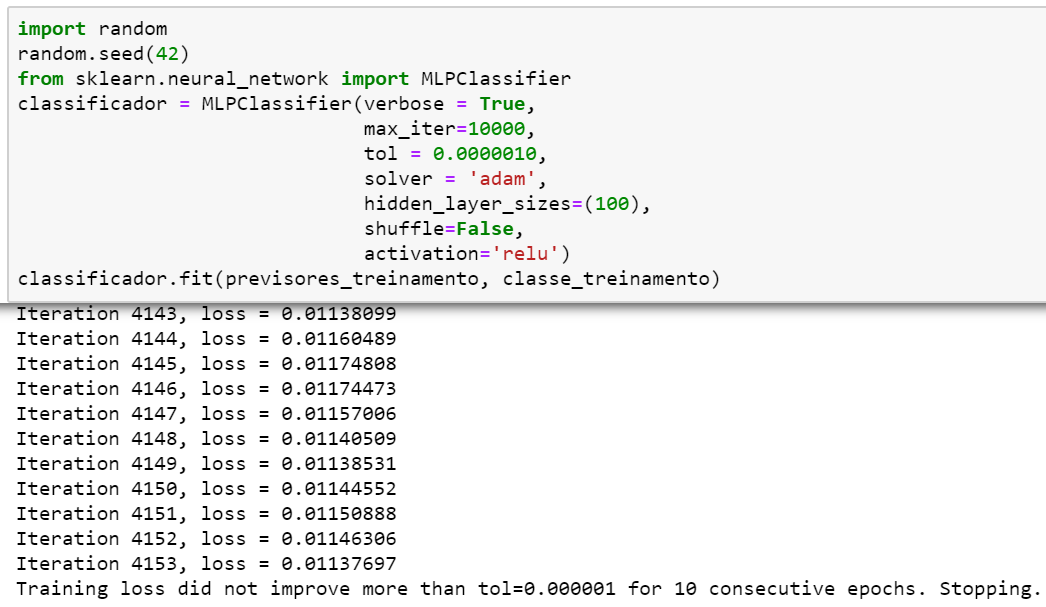
\includegraphics[width=.7\textwidth]{imagens/mlp_classifier.png}
	\caption{Código do \textbf{MLPClassifier}}
	\label{fig:mlp_classifier}
	{\scriptsize Fonte: compilação do autor}
\end{figure}

A figura \ref{fig:validacao_notebook} mostra algumas métricas de validação após o modelo criado realizar as predições na base de teste (25\% do dataset ou 71 políticas). Nela, pode-se perceber a acurácia do classificador em 95.77\%, classificando, conforme a matriz de confusão mostrada na mesma figura, somente 3 previsões incorretas. Levando-se em conta que o modelo se aprimora conforme a quantidade de instâncias aumenta, de acordo com o pressuposto no\textit{ teorema da aproximação universal} \cite{hagan_neural_1996}, pode se considerar este como um modelo satisfatório.

\begin{figure}[h!]
	\centering
	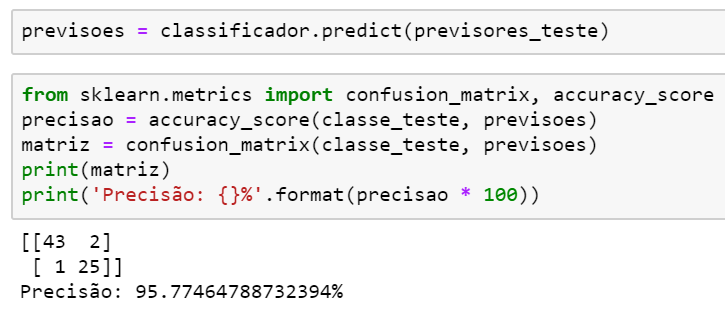
\includegraphics[width=.6\textwidth]{imagens/validacao_notebook.png}
	\caption{Validações para o modelo \textbf{MLPClassifier}}
	\label{fig:validacao_notebook}
	{\scriptsize Fonte: compilação do autor}
\end{figure}

A figura \ref{fig:dimensionalidade} mostra a dimensionalidade dos dados após transformados pelo processo de padronização e dá uma visão geral de 3 atributos, \textit{\textbf{sujeito, ação e objeto}} e o impacto na difusão dos conflitos no espaço após os atributos categóricos terem sido, todos, transformados para uma representação numérica.

\begin{figure}[h!]
	\centering
	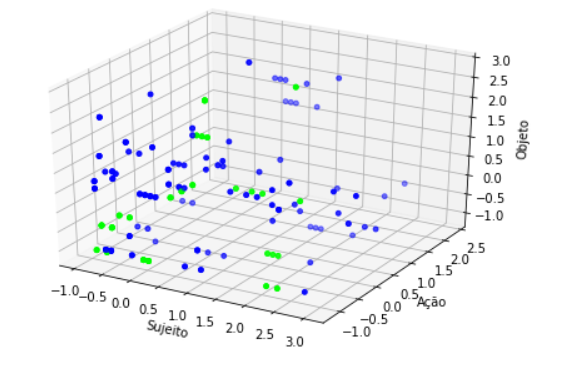
\includegraphics[width=.6\textwidth]{imagens/dimensionalidade.png}
	\caption{Dimensionalidade dos dados: atributos sujeito, ação e objeto}
	\label{fig:dimensionalidade}
	{\scriptsize Fonte: compilação do autor}
\end{figure}

\subsection{Experimentos com TensorFlow e Pytorch}
De acordo com \cite[p. 233]{geron_maos_2020}, o \textit{TensorFlow} é uma biblioteca de software para cálculo numérico de código aberto especialmente adequada e ajustada para o Aprendizado de Máquina em larga escala. Foi desenvolvido pela \textit{Google Brain Team} para uso intensivo de redes neurais profundas. O código fonte foi disponibilizado em 2015 e está à disposição no link: \underline{\texttt{https://github.com/tensorflow/tensorflow}}.

É possível usar computação paralela em várias CPU's ou GPU's além de suportar computação distribuída para que seja possível o treinamento e o uso de redes neurais em grandes conjuntos de treinamento dividindo os cálculos por centenas de servidores em um período de tempo razoável. \cite{geron_maos_2020}. 

Entre suas características importantes destacam-se: rodar em diversos sistemas operacionais (e inclusive na nuvem); diversas APIs públicas para criação, treinamento e avaliação de arquiteturas de diferentes tipos de redes neurais; diversas outras API's de alto nível foram construídas com base no TensorFlow como o \textit{Keras} e o \textit{Pretty Tensor}; implementações em C++ altamente eficientes para operações de Aprendizado de Máquina; nós de otimização avançados para procura por parâmetros que minimizem uma função de custo; usa extensões CUDA, uma  API destinada a computação paralela, GPGPU, e computação heterogênea, criada pela Nvidia que dá acesso ao conjunto de instruções virtuais da GPU e a elementos de computação paralela. \cite{geron_maos_2020}.

Os cálculos no \textit{TensorFlow} são expressos como grafos de fluxo de dados , seu nome deriva das operações que as redes neurais realizam em arranjos de dados multidimensionais, chamados de ``tensores''(generalização matemática de escalares, vetores e matrizes). \cite{kadimisetty_tensorflow_2018}

Foi realizado, assim, no escopo deste trabalho experimentos com a base de dados de com 281 políticas já citada anteriormente. O notebook completo está disponível online no endereço: \underline{\texttt{https://bit.ly/33BmCzt}}. Foi todo construído no ambiente Google Collab que é um serviço de nuvem gratuito hospedado pelo Google para incentivar a pesquisa de Aprendizado de Máquina e Inteligência Artificial, similar ao Jupyter Notebook, é uma lista de células que podem conter textos explicativos ou códigos executáveis e suas saídas. \cite{collab_2020}.

Neste modelo os hiperparâmetros principais foram ajustados como: tamanho do batch em 20 (analisa, computa e reajusta os pesos de 20 instâncias de cada vez, por época), o número de GPU's trabalhando em conjunto para 4, a taxa de aprendizado em 0.00001, o decaimento dos pesos em 0.000005 e o número de épocas padrão em 30 (apenas para testes inciais).

\begin{figure}[h!]
	\centering
	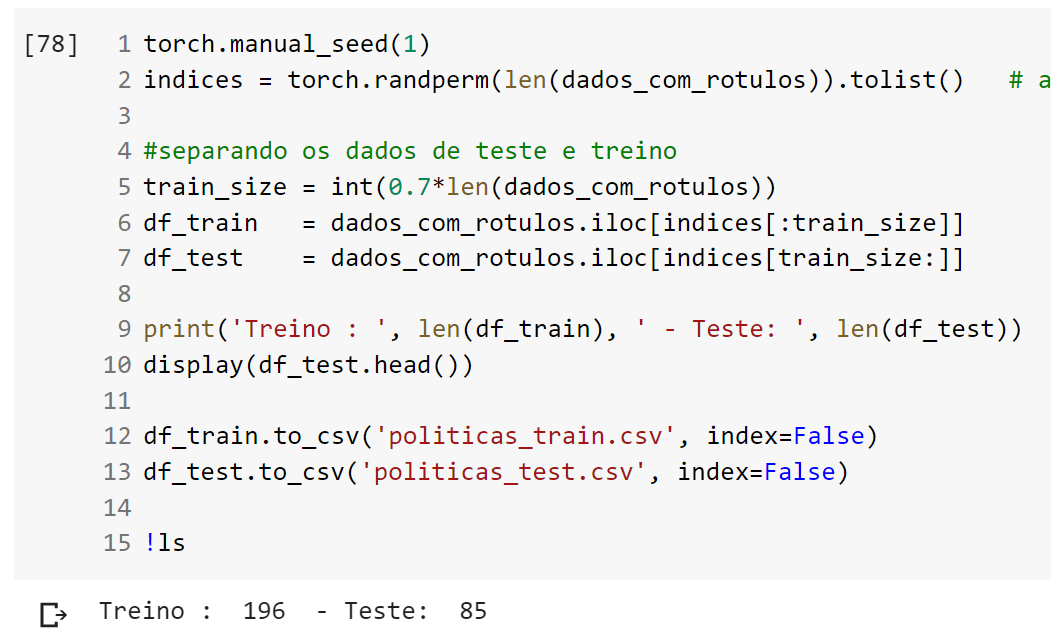
\includegraphics[width=.6\textwidth]{imagens/separacao-teste-treino.png}
	\caption{Separação dos dados de teste e treino}
	\label{fig:separacao-teste-treino}
	{\scriptsize Fonte: compilação do autor}
\end{figure}

Para o processo de validação, usou-se o \textit{holdout} com a separação em 70\% das instâncias para o treinamento da rede neural e 25\% para teste, predição e validação. Na figura \ref{fig:separacao-teste-treino} pode-se visualizar como o processo foi realizado,inclusive com a quantidade de instâncias em cada conjunto de dados (na linha 2 é feita a randomização do \textit{dataset} original para evitar o overfitting e balancear a probabilidade da distribuição).

O pacote \texttt{torch.util.data} do PyTorch possui a classe abstrata \texttt{Dataset}. Ela permite que seja implementado o próprio dataset reescrevendo os métodos: 

\begin{itemize}
	\item \texttt{\_\_init\_\_(self)}: Define a lista de amostras do dataset
	\item \texttt{\_\_getitem\_\_(self, idx)}: Carrega uma amostra, aplica as devidas transformações e retorna uma tupla (dado, rótulo)
	\item \texttt{\_\_len\_\_(self}): Retorna a quantidade de amostras do dataset
\end{itemize}

Dessa forma, a figura \ref{fig:classe-politicas} mostra a elaboração de uma classe chamada \texttt{Politicas} que implementa uma classe-filha que herda da superclasse, \textit{Dataset} descrita acima.

\begin{figure}[h!]
	\centering
	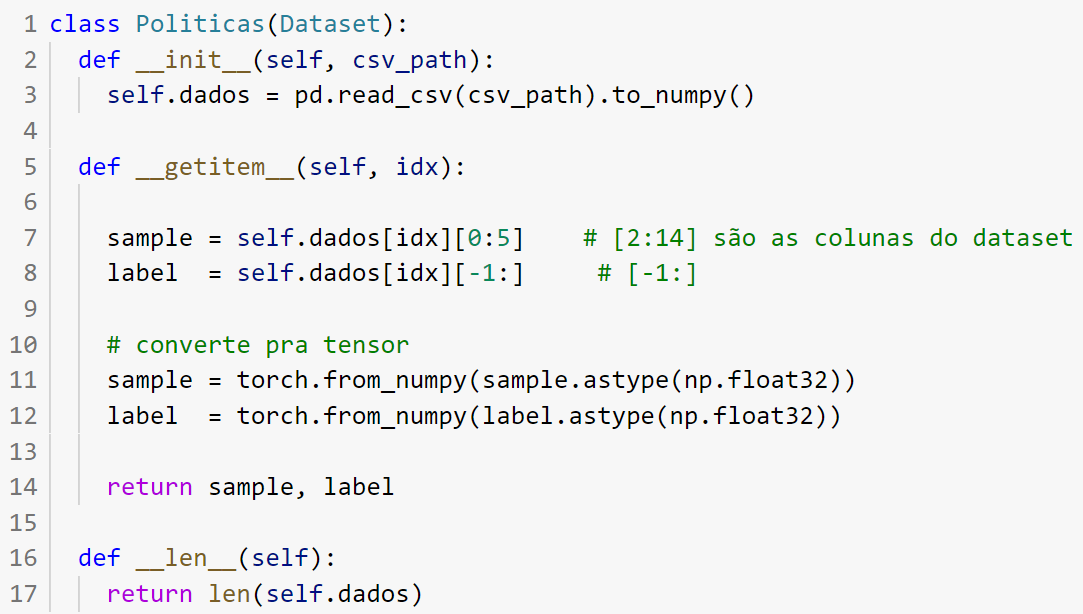
\includegraphics[width=.6\textwidth]{imagens/classe-politicas.png}
	\caption{Implementação da classe Politicas}
	\label{fig:classe-politicas}
	{\scriptsize Fonte: compilação do autor}
\end{figure}

Em seguida, dois objetos DataLoader são criados, um para a base de treinamento e um para a base de teste. Em seguida, a Rede Neural Multicamadas é instanciada mediante a criação de uma classe chamada MLP que herda da classe \texttt{nn.Module} que representa um módulo genérico de uma rede neural. 

A arquitetura da rede é configurada dentro da classe que a cria sendo: uma camada linear de entrada, duas camadas lineares ocultas com 32 neurônios em cada camada usando a função de ativação ReLU e uma camada linear de saída com dois neurônios, representando os dois rótulos do atributo que é a classe, neste caso específico, o atributo binário \textbf{conflito} que será predito. É criada, no mesmo código da classe MLP, uma função que faz o avanço (fed-forward) das computações na rede e, ao final, é instanciada uma variável chamada \texttt{net} com as variáveis descritas: 5 atributos/neurônios na camada linear de entrada, 2 camadas ocultas com 32 neurônios cada e 2 camadas de saída representando as variáveis preditas. Na mesma linha que cria o objeto \texttt{net} é feito o \textit{cast} da rede na GPU para que ela possa, ao ser treinada, fazer uso dos poderes computacionais em paralelo da API, CUDA. A figura \ref{fig:mlp-pytorch} mostra o código descrito aqui.

\begin{figure}[h!]
	\centering
	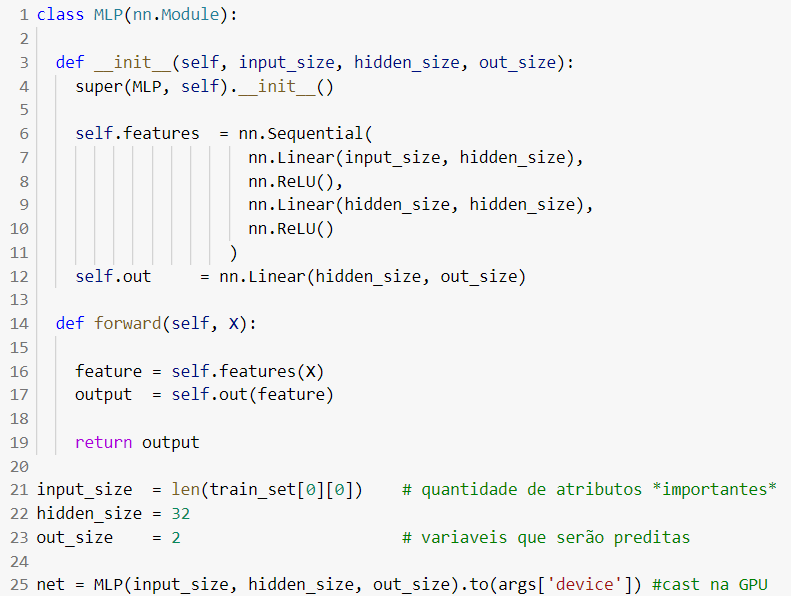
\includegraphics[width=.6\textwidth]{imagens/mlp-pytorch.png}
	\caption{Implementação da classe que modela a arquitetura da rede}
	\label{fig:mlp-pytorch}
	{\scriptsize Fonte: compilação do autor}
\end{figure}

Em seguida é definida uma \textit{loss function}(função de perda ou de custo). É criado um critério que mede o erro médio quadrático (norma matricial ao quadrado) entre cada elemento na entrada $x$ e o destino $y$. O otimizador utilizado é o Adam, um algoritmo para otimização estocástica descrito em \cite{adam_2017} passando para o algoritmo os valores da taxa de aprendizado e do decaimento de pesos mostrado anteriormente nesta seção.

O fluxo de treinamento desta arquitetura de rede neural multicamadas proposta neste experimento segue o algoritmo iterativo:

\begin{itemize}
	\item Iterar nas épocas
	\item Iterar nos batches (a quantidade de instâncias simultâneas)
	\item Cast dos dados no dispositivo de hardware (GPU)
	\item Forward na rede e cálculo da \textit{loss function}
	\item Cálculo do gradiente e atualização dos pesos
\end{itemize}

Esse conjunto de passos é responsável pelo processo iterativo de otimização de uma rede. A validação, entretanto, é apenas a aplicação da rede em dados nunca antes vistos para estimar a qualidade do modelo no mundo real.

Três funções, portanto, são criadas, uma para modelar o treinamento da rede neural, uma para o teste e validação e outra que agrega as duas primeiras em uma só para executar o algoritmo descrito anteriormente. Então, para finalizar o experimento com o TensorFlow, o PyTorch, CUDA e o Google Collaboratory, foi realizado um treinamento com 500 épocas da rede neural explanada nesta seção e os resultados tanto do treino quando do teste e validação foram armazenados.

As figuras \ref{fig:train}, \ref{fig:test} e \ref{fig:forward} mostram as três funções citadas anteriormente

Como esclarecimento e interpretação visual foi construída, pois, a figura \ref{fig:convergencia} com os dados de armazenados de treino e teste (média da \textit{loss function} ou função de custo de cada iteração dentro da época) que mostra um comparativo das épocas de teste e treino da rede neural e a convergência de ambas, retratando a acurácia e a validade do modelo deste experimento.

\begin{figure}[h!]
	\centering
	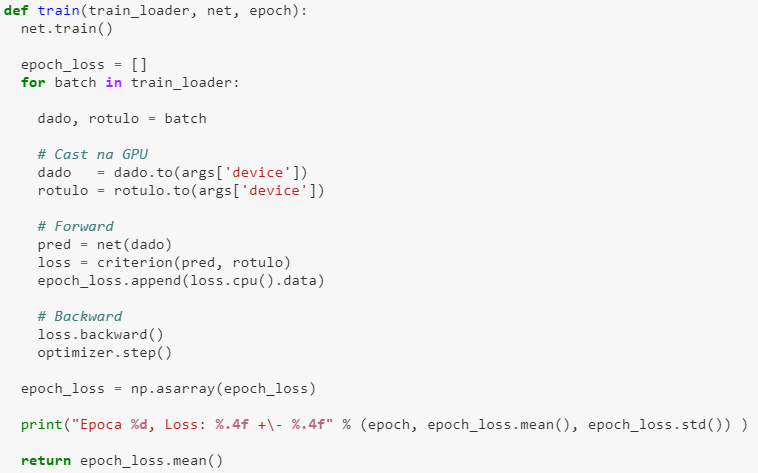
\includegraphics[width=.6\textwidth]{imagens/train.png}
	\caption{Implementação da função de treino da rede}
	\label{fig:train}
	{\scriptsize Fonte: compilação do autor}
\end{figure}

\begin{figure}[h!]
	\centering
	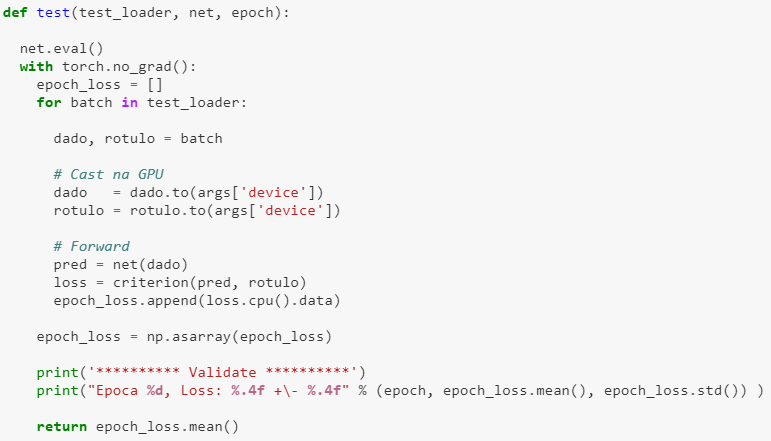
\includegraphics[width=.6\textwidth]{imagens/test.png}
	\caption{Implementação da função de teste da rede}
	\label{fig:test}
	{\scriptsize Fonte: compilação do autor}
\end{figure}

\begin{figure}[h!]
	\centering
	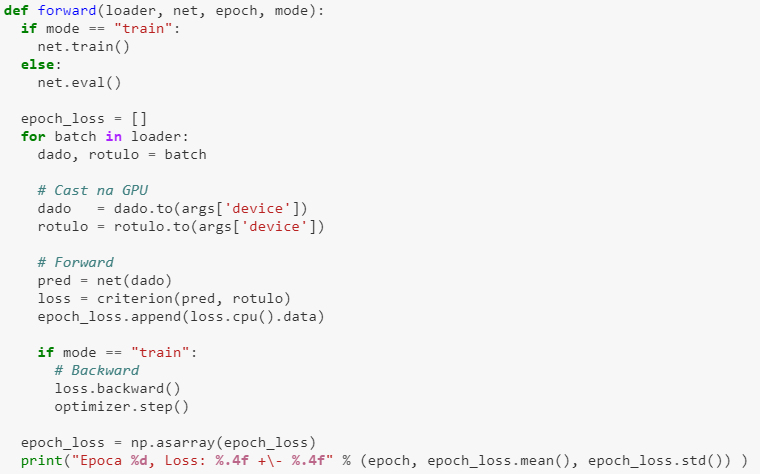
\includegraphics[width=.6\textwidth]{imagens/forward.png}
	\caption{Implementação da função que mescla o treino e o teste em uma só}
	\label{fig:forward}
	{\scriptsize Fonte: compilação do autor}
\end{figure}

\begin{figure}[h!]
	\centering
	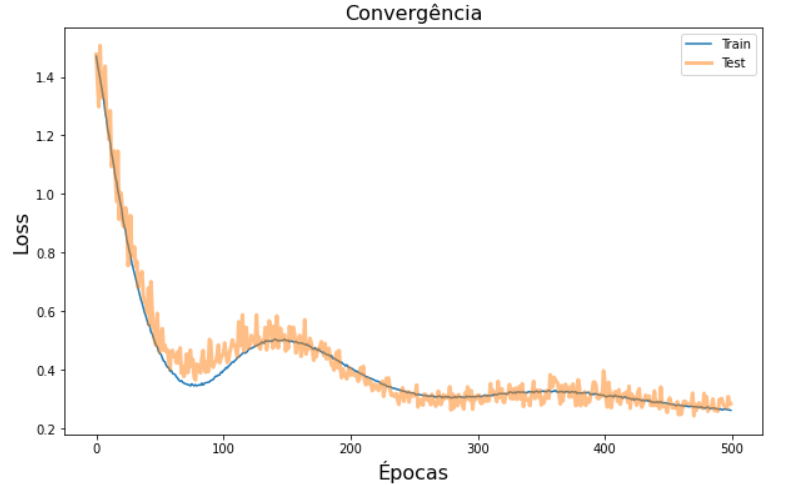
\includegraphics[width=.6\textwidth]{imagens/convergencia.png}
	\caption{Convergência das épocas entre o treino e o teste da MLP}
	\label{fig:convergencia}
	{\scriptsize Fonte: compilação do autor}
\end{figure}

\subsection{Análise dos resultados}\label{analise_resultados}
Os experimentos realizados na seção \ref{resultados} corroboram a hipótese de que a detecção de conflitos pode ser transformada em um problema da tarefa de classificação da mineração de dados e do aprendizado de máquina. As vantagens sobre as outras abordagens relatadas na literatura são:
\begin{itemize}
	\item A detecção do conflito pode ser realizada em tempo de execução, pois os modelos já estão treinados;	
	\item As políticas são verificadas ``em lote'' e não em pares já que a análise em pares é um problema computacionalmente custoso da classe NP-Completo como demonstrado por \cite{shoham_tennenholtz_1995}; 
	\item Ambas as técnicas analisadas neste trabalho mostraram-se eficazes com acurácias acima da proposta inicialmente (95\%);
	\item os modelos de machine learning desenvolvidos nos experimentos podem ser aplicados em outros contextos, pois são suficientemente genéricos para tal;
	\item Ao analisar uma nova política, não é necessário ``varrer'' ou consultar todas as instâncias do \textit{dataset} novamente já que os modelos já estão treinados;
	\item os modelos de machine learning tem a tendência a melhorarem a eficácia à medida que a quantidade de instâncias cresce
\end{itemize}

Todas os modelos e algoritmos demonstrados nos experimentos tiveram acurácia acima de 95\% o que mostra que a detecção de conflitos em políticas (ou normas) pode ser colocada como uma classe de problemas a serem resolvidos de forma eficiente por técnicas de aprendizagem de máquina.

\chapter{Cronograma e propostas para o texto final}\label{propostas}
Para a pesquisa que resultará na dissertação de mestrado os seguintes pontos serão levantados, estudados e melhor definidos em termos dos objetivos do trabalho:
\begin{enumerate}
\item Finalização da pesquisa teórica sobre o relacionamento de entidades;
\item Finalização da pesquisa teórica sobre funções de custo, SVM, descida do gradiente, topologias de redes neurais, suporte matemático aprofundado para o SVM;
\item estudo de outras redes, como Adaline, Madaline, redes de Kohonen, redes RBF e compará-las com as MLP e o SVM ;
\item Análise matemática profunda das outas função de ativação no classificador;
\item Análise teórica e implementação de outros otimizadores;
\item Realizar mais experimentos redes neurais e SVM;
\item Comparação final com outros classificadores (preferencialmente, geométricos, como o KNN e o SVM, avaliando suas acurácias e eficiência (para os conflitos indiretos).
\end{enumerate}
Para isso, propõem-se o seguinte cronograma descrito na tabela \ref{tab:cronograma}

\begin{table}[]
	\caption{Cronograma de finalização da dissertação}
	\label{tab:cronograma}
	\begin{tabular}{lccccccc}
		\hline
		\textbf{Atividades} & \textbf{\begin{tabular}[c]{@{}c@{}}1ª \\ sem\\ ago\end{tabular}} & \textbf{\begin{tabular}[c]{@{}c@{}}2ª \\ sem\\ ago\end{tabular}} & \textbf{\begin{tabular}[c]{@{}c@{}}1ª \\ sem\\ set\end{tabular}} & \textbf{\begin{tabular}[c]{@{}c@{}}2ª \\ sem\\ set\end{tabular}} & \textbf{\begin{tabular}[c]{@{}c@{}}1ª \\ sem\\ out\end{tabular}} & \textbf{\begin{tabular}[c]{@{}c@{}}2ª \\ sem\\ out\end{tabular}} & \textbf{\begin{tabular}[c]{@{}c@{}}1ª\\ sem\\ nov\end{tabular}} \\ \hline
		\begin{tabular}[c]{@{}l@{}}Finalização da pesquisa \\ teórica sobre o relacionamento\\ de entidades\end{tabular} & X & X &  &  &  &  &  \\
		\begin{tabular}[c]{@{}l@{}}Finalização da pesquisa teórica\\ sobre funções de custo, SVM, \\ descida do gradiente, topologias\\ de redes neurais, suporte \\ matemático aprofundado para \\ o SVM;\end{tabular} & X & X &  &  &  &  &  \\
		\begin{tabular}[c]{@{}l@{}}Estudo de outras redes, como \\ Adaline, Madaline, redes de \\ Kohonen, redes RBF e \\ compará-las com as MLP \\ e o SVM\end{tabular} &  & X & X & X &  &  &  \\
		\begin{tabular}[c]{@{}l@{}}Análise matemática profunda\\ das outras função de\\ ativação no classificador\end{tabular} &  &  & X & X &  &  &  \\
		\begin{tabular}[c]{@{}l@{}}Análise teórica e implementação\\ de outros otimizadores\end{tabular} &  &  & X & X & X &  &  \\
		\begin{tabular}[c]{@{}l@{}}Realizar mais experimentos redes \\ neurais e SVM\end{tabular} &  &  & X & X & X &  &  \\
		\begin{tabular}[c]{@{}l@{}}Comparação final com outros \\ classificadores (preferencialmente,\\ geométricos, como o KNN e o SVM,\\ avaliando suas acurácias e eficiência \\ (para os conflitos indiretos)\end{tabular} &  &  &  & X & X &  &  \\
		\begin{tabular}[c]{@{}l@{}}Escrita, revisão e entrega de \\ resultados iniciais\end{tabular} &  &  &  &  & X & X & X \\
		Texto final com resultados &  &  &  &  &  & X & X \\ \hline
	\end{tabular}
\end{table}

\chapter{Conclusões}\label{conclusoes}
\begin{itemize}
	\item Esta pesquisa mostrou que é possível \textit{converter a detecção de conflitos a um problema de classificação} especificamente, para os conflitos \textbf{\textit{diretos}};
	\item O classificador mais acurado, nos experimentos, foi, como se imaginava pela hipótese, o \textit{MultiLayer Perceptron} que é um classificador que usa \textit{backpropagation} para aprender usando perceptron de várias camadas para classificar instâncias desconhecidas \cite{eibe2016};
	\item Será realizada uma comparação entre o MLP e o SVM (e outros classificadores geométricos). Suas acurácias serão devidamente comparadas juntamente com a eficiência das soluções propostas.
	\item Todas os modelos e algoritmos demonstrados nos experimentos tiveram acurácia acima de 95\% o que mostra, portanto, que a detecção de conflitos em políticas pode ser colocada como uma classe de problemas a serem resolvidos de forma eficiente por técnicas de aprendizagem de máquina.
\end{itemize}
%\chapter{Conteúdos específicos do modelo de trabalho %acadêmico}\label{cap_trabalho_academico}
%
%\section{Quadros}
%
%Este modelo vem com o ambiente \texttt{quadro} e impressão de Lista de quadros 
%configurados por padrão. Verifique um exemplo de utilização:
%
%\begin{quadro}[htb]
%\caption{\label{quadro_exemplo}Exemplo de quadro}
%\begin{tabular}{|c|c|c|c|}
%	\hline
%	\textbf{Pessoa} & \textbf{Idade} & \textbf{Peso} & \textbf{Altura} \\ \hline
%	Marcos & 26    & 68   & 178    \\ \hline
%	Ivone  & 22    & 57   & 162    \\ \hline
%	...    & ...   & ...  & ...    \\ \hline
%	Sueli  & 40    & 65   & 153    \\ \hline
%\end{tabular}
%\fonte{Autor.}
%\end{quadro}

%Este parágrafo apresenta como referenciar o quadro no texto, requisito
%obrigatório da ABNT. 
%Primeira opção, utilizando \texttt{autoref}: Ver o \autoref{quadro_exemplo}. 
%Segunda opção, utilizando  \texttt{ref}: Ver o Quadro \ref{quadro_exemplo}.

% ----------------------------------------------------------
% PARTE
% ----------------------------------------------------------
%\part{Referenciais teóricos}
% ----------------------------------------------------------

% ---
% Capitulo de revisão de literatura
% ---
%\chapter{Lorem ipsum dolor sit amet}
% ---

% ---
%\section{Aliquam vestibulum fringilla lorem}
% ---

%\lipsum[1]

%\lipsum[2-3]

% ----------------------------------------------------------
% PARTE
% ----------------------------------------------------------
%\part{Resultados}
% ----------------------------------------------------------

% ---
% primeiro capitulo de Resultados
% ---
%\chapter{Lectus lobortis condimentum}
% ---

% ---
%\section{Vestibulum ante ipsum primis in faucibus orci luctus et ultrices
%posuere cubilia Curae}
% ---

%\lipsum[21-22]

% ---
% segundo capitulo de Resultados
% ---
%\chapter{Nam sed tellus sit amet lectus urna ullamcorper tristique interdum
%elementum}
% ---

% ---
%\section{Pellentesque sit amet pede ac sem eleifend consectetuer}
% ---

%\lipsum[24]

% ----------------------------------------------------------
% Finaliza a parte no bookmark do PDF
% para que se inicie o bookmark na raiz
% e adiciona espaço de parte no Sumário
% ----------------------------------------------------------
\phantompart

% ---
% Conclusão
% ---
%\chapter{Conclusão}
% ---

%\lipsum[31-33]

% ----------------------------------------------------------
% ELEMENTOS PÓS-TEXTUAIS
% ----------------------------------------------------------
\postextual
% ----------------------------------------------------------

% ----------------------------------------------------------
% Referências bibliográficas
% ----------------------------------------------------------
\bibliography{bibliografia}

% ----------------------------------------------------------
% Glossário
% ----------------------------------------------------------
%
% Consulte o manual da classe abntex2 para orientações sobre o glossário.
%
%\glossary

% ----------------------------------------------------------
% Apêndices
% ----------------------------------------------------------

% ---
% Inicia os apêndices
% ---
%\begin{apendicesenv}

% Imprime uma página indicando o início dos apêndices
%\partapendices

% ----------------------------------------------------------
%\chapter{Quisque libero justo}
% ----------------------------------------------------------

%\lipsum[50]

% ----------------------------------------------------------
%\chapter{Nullam elementum urna vel imperdiet sodales elit ipsum pharetra ligula
%ac pretium ante justo a nulla curabitur tristique arcu eu metus}
% ----------------------------------------------------------
%\lipsum[55-57]

%\end{apendicesenv}
% ---


% ----------------------------------------------------------
% Anexos
% ----------------------------------------------------------

% ---
% Inicia os anexos
% ---
%\begin{anexosenv}

% Imprime uma página indicando o início dos anexos
%\partanexos

% ---
%\chapter{Morbi ultrices rutrum lorem.}
% ---
%\lipsum[30]

% ---
%\chapter{Cras non urna sed feugiat cum sociis natoque penatibus et magnis dis
%parturient montes nascetur ridiculus mus}
% ---

%\lipsum[31]

% ---
%\chapter{Fusce facilisis lacinia dui}
% ---

%\lipsum[32]

%\end{anexosenv}

%---------------------------------------------------------------------
% INDICE REMISSIVO
%---------------------------------------------------------------------
\phantompart
\printindex
%---------------------------------------------------------------------

\end{document}
